\chapter{Lagrangian Structural Topology optimization}
\minitoc
\begin{mdframed}[hidealllines=true,backgroundcolor=lightgray!20]
\section*{Résumé}
Dans ce chapitre nous passons en revue les approches d'optimisation topologique dites lagrangiennes ou bien explicites. Dans cette famille d'approches la solution est décrite par un ensemble de composantes de forme simple dont les dimensions, positions et orientations sont données comme variables de design. Entre les approches qu'on peut retrouver dans la littérature on considère:
 \begin{itemize}
 \item \textbf{MMC}: \textit{Methode of Moving Morphable Components} avec modèle matériau d'Esartz.
 \item \textbf{GP}: \textit{Geometry Projection}
 \item \textbf{MNA}: \textit{Moving Node Approach}
 \end{itemize}
 Une nouvelle techniques appelée \textit{Generalized Geometry Projection} (\textbf{GGP}) \cite{coniglio2019generalized} est proposée. Cet approche est en réalité une généralisation de l'approche de GP qui permet de représenter toutes les techniques mentionnées précédemment. En plus cette technique offre la possibilité d'éviter l'apparition de points d'inflexion dans les réponses obtenues utilisant la projection sur maillage éléments finis. Ensuite un étude bibliographique et comparative des approches les plus courantes pour l'assemblage géométrique de composantes est aussi proposée. Le calcul analytique des gradients est ensuite déduit.
 Différents cas simplifiés démontrent l'efficacité de l'approche proposée pour éviter les points d'inflexion. 
 Ensuite les contraintes de stress sont aussi traitées par la formulation unifiée d'agrégation et relaxation de \cite{verbart2017unified}. Finalement l'application  de l'approche MNA au problème de design du mât et attaches moteur, déjà traité dans le chapitre \ref{chap:2} par la méthode SIMP, est considérée. D'abord des composantes rectangulaires ensuite des composantes  spécifiques au problème en étude sont traitées. 
\end{mdframed}
\label{chap:3}
    SIMP direct density based approaches to topology optimization \cite{bendsoe1989optimal,zhou1991coc,bendsoe1995optimization}, such as the one in chapter \ref{chap:2}, are currently among the most popular ones. The exploration power of these approaches, their freedom and their ease in handling large changes in the design configuration without re-meshing come however at the cost of some drawbacks as well:
     \begin{itemize} 
   \item The number of design variables and of degrees of freedoms in the finite element model grows quite fast in 3D problems and their resolution becomes quickly prohibitive especially if considering optimization formulation that do not only include compliance and volume fraction. \item The typical "organic" designs obtained with direct density based methods, even if highly effective, may not be easily compatible with manufacturing requirements (e.g. casting, rolling, overhang angle constraints, etc.). Indeed as analyzed in the recent survey by Liu and Ma \cite{liu2016survey}, and more recently of Liu et al. \cite{liu_current_2018} the implementation of manufacturing considerations in topology optimization is still a challenging, highly active area of research.  
   \item Intermediate densities often subsist in the final design in direct density based approaches due to computational cost constraints, preventing the full convergence towards black and white designs. The gray elements would then have to be threshold to black and white solutions, which can lead to a loss in performance compared to the optimum.  
   \item The density formulation of the topology optimization problem is ill posed and need to be transformed into a well posed one through restriction to feasible set of solutions \cite{borrvall2001topology}. Some approaches like mesh independent filter techniques \cite{sigmund1994design}, depending on the filter size, can be computationally expensive.
   \end{itemize}

An alternative family of approaches seeks to both use geometric primitives (i.e. geometric components) to define the optimal solution and inherit a fixed mesh as typical in direct density based topology optimization such as SIMP. In the literature one can find two major groups of approaches incorporating geometric features in topology optimization: 
\begin{itemize}
    \item A first group combines the free-form topology optimization with embedded components or holes shaped as geometric primitives. (c.f. Chen et al. \cite{chen2007shape};Qian and Ananthasuresh \cite{qian2004optimal}; Xia et al. \cite{xia2012sensitivity}; Zhang et al. \cite{zhang2011some,zhang2015explicit}; Zhou and Wang \cite{zhou2013engineering}; Zhu et al. \cite{zhu2008simultaneous})
    \item A second group, to which this work belongs, represents the solution only by means of geometric primitives.
    Norato \cite{norato2018topology} provides an extensive description of works dealing with these approaches. The precursor of these methods is the bubble method (Eschenauer et al. \cite{eschenauer1994bubble}), one of the first form of topology optimization. Still this approach requires re-meshing during the optimization process which affects its computational burden. Another work that can be consider as belonging to this category is the Feature-based topology optimization \cite{cheng2006feature}, where the structure is obtained as the results of Boolean operations over simple geometric feature structures, in this case holes. The same author proposes  in \cite{chen2008shape} an implicit control of the solution quality using a quadratic term of the energy in the formulation of the optimization problem. In the work of Seo et al. \cite{seo2010isogeometric}, the solution is described using  trimmed spline surfaces and the isogeometric analysis. In the Adaptive Mask
    Overlay Topology Synthesis
    Method, Saxena et al. \cite{saxena2011circular} circular, rectangular or elliptical holes are considered in the solution and the structural analysis is performed on the remaining solid structure using hexagonal elements.
    A similar approach is applied by Wang et al. \cite{wang2012high}: a fixed mesh is employed this time and a regularized Heaviside function is used to evaluate the mechanical properties on a fixed finite element mesh. Liu et al. \cite{liu2014level} proposed to use Compactly supported Radial basis functions to interpolate simple geometric features in a level set topology optimization framework. The performance of the resulting structure was then computed thanks to the extended finite element method (XFEM). 
    In the ISOCOMP approach of Lin et al. \cite{lin2015isocomp}, 
    the simultaneous optimization of both the location of holes and the layout of material is studied with the use of both isogeometric analysis and the Hierarchical Partition of Unity Field Compositions (HPFC) theory, which is employed for both geometry and solution field approximations.
    \\ 
\end{itemize}

In this second family of methods, four approaches represent a solution as the union of geometric entities that can move, stretch and analytically modify their shapes: the moving morphable components (MMC) method (Guo et al.  \cite{guo2014doing,guo2016explicit}, Zhang et al. \cite{zhang2016new,zhang2017new}) ; the geometry projection (GP) method (Bell et al. \cite{bell2012geometry}, Norato et al. \cite{norato2015geometry}, Zhang et al. \cite{zhang2016geometry}); the Method of Moving Morphable Bars (MMB) Hoang et al. \cite{hoang2017topology} and the Moving Node Approach (MNA), introduced in the Master thesis of Overvelde \cite{overvelde2012moving}. We refer to these approaches as explicit topology optimization approaches, highlighting the fact that the material description is explicitly described, instead of implicitly as it is the case for direct density based approaches, where the layout is describe by a mapping of presence and absence of material. In \cite{guo2014doing}, an explicit level set function is used to determine the geometry of moving morphable components with uniform thickness. The XFEM approach was employed as an alternative for the displacement computation \cite{kreissl2012levelset,van2007stress,wei2010study}. The same framework is also presented in Zhang et al. \cite{zhang2016lagrangian} where MMC is identified as a way of extending techniques commonly employed in shape optimization, with the freedom inherited from topology optimization.  Moving components with variable thickness are used in \cite{zhang2016new}, and the Esartz material model is employed to enhance computational efficiency. In the work of Zhang et al. \cite{zhang2016minimum} length scale control is achieved by directly controlling the component's minimal thickness.
In Deng et al. \cite{deng2016design} the MMC approach is successfully implemented to solve various types of problems, like the design of compliant mechanisms and of low-frequency resonating micro devices.
In the work of Zhang et al. \cite{zhang2017new}, the MMC framework is extended to 3D structures.
The complexity of the solution is controlled in \cite{zhang2017structural} by controlling the maximum number of components in the final solutions.

The Moving Morphable Voids approach \cite{zhang2017explicit} makes use of b-splined shaped holes, explicitly piloted in the topology optimization. The proposed framework, not only reduces the optimization burden due to variables reduction, but also impacts the cost of the evaluation of the displacement field, eliminating the element completely contained in the void region from the analysis. The same framework is applied to tackle stress based topology optimization in \cite{zhang2018moving}.
In Zhang et al. \cite{zhang2017structuralo} the control of the solution is achieved by varying explicitly the boundaries of Components or voids using B-spline curves.  
In Takalloozadeh et al. \cite{takalloozadeh2017implementation} the topological derivative is implemented in the MMC approach.
 In the work of \cite{guo2017self} the ability of MMC to determined self-supported structures is studied and in Liu et al. \cite{liu2017additive} the MMCs/MMVs framework is employed to determine graded lattice structures achievable with additive layer manufacturing technologies. In Hou et al. \cite{hou2017explicit} the MMC framework is proposed based on Isogeoemtric Analysis (IGA) instead of finite element analysis (FEA). In Zhang et al. \cite{zhang2018topology}, the MMC approach is employed to design multi-material structures and in Zhang et al. \cite{zhang2018movings} it is employed to find the best layout of stiffening ribs including buckling constraints. Geometric non-linearities are considered in Zhu et al. \cite{zhu2018structural} for MMC and in Xue et al. \cite{xue2019explicit} for MMV.
  In Lei et al. \cite{lei2019machine} machine learning techniques like:  support vector regression (SVR) \cite{smola2004tutorial} and the K-nearest-neighbors (KNN) \cite{altman1992introduction}, were adopted in order to speed up the resolution of the optimization problem, under MMC framework. In Liu et al. \cite{liu2018efficient} an efficient strategy is proposed to decouple the finite element mesh discretization from the discretization employed to assemble the stiffness matrix on the basis of the geometric configuration.
  In Sun et al. \cite{sun2018topology} the topology optimization of a 3D multi-body systems considering large deformations and large overall motion is achieved using MMC.\\  
With the Method of Moving Morphable Bars (MMB) Hoang et al. \cite{hoang2017topology} introduce round ended bars in the topology optimization framework that can overlap and change both shape and position. As main features of this work one can identify the control of both minimal and maximal thickness of the components, the use of sigmoid Heaviside function to project the components on the fixed finite element mesh, the use of SIMP material model to penalize intermediate density and the Boolean union of components realized making the product of Heaviside functions. MMB was also studied in Wang et al. \cite{wang2018explicit} for the layout of planar multi-component systems. \\
The Geometry Projection (GP) approach was initially introduced by Norato et al. \cite{norato2004geometry}, for the shape optimization of holes over a fixed finite element mesh. This basic idea was developed further by Bell et al. \cite{bell2012geometry} to make the topology optimization of structures composed by rectangular components in 2D, by Norato et al. \cite{norato2015geometryde} using 2D round ended bar components that can both overlap and merge. The same author proposed to use this approach to find the best distribution of short fiber reinforcement in \cite{norato2015geometry}. In Zhang et al. \cite{zhang2016geometry} Geometry projection approach was implemented for 3D solid structures composed of rectangular plates. In Zhang et al. \cite{zhang2017stress} stress based topology optimization is conducted on 2D topology optimization problems, using GP. The design of unit cells for lattice materials in 3D is considered in Watts et al. \cite{watts2017geometric}. In Zhang et al. \cite{zhang2018geometry} curved plates are considered as building blocks of 3D topology optimization problems using GP.
In Zhang et al. \cite{zhang2017optimal} Geometry Projection was employed to design the rib reinforcement of plates in 3D.
In the work of Norato \cite{norato2018topology} supershapes geometric features are employed as building blocks in a 2D topology optimization framework based on geometry projection. 
In Kazemi et al. \cite{kazemi2018topology}, the Geometry Projection was applied to multi-material design of 2D and 3D structures.  
In Zhang et al. \cite{zhang2018finding} a tunneling strategy is proposed to alleviate the initial point dependency in Geometry projection.

We chose to focus in this chapter on the following three frameworks, which follow different approaches for achieving explicit topology optimization of 2D and 3D structures: the Moving Morphable Components (MMC) with Esartz material approach, the Geometry Projection (GP) approach and Moving Node Approach (MNA). In this chapter we also propose a new general framework that we call Generalized Geometry Projection (GGP), of which all three approaches can be seen as particular cases. A further contribution resides in the proposal of a specific saturation strategy that can be adopted to overcome the difficulties that can be encountered in the assembly of geometric features, required in all considered explicit topology optimization approaches. Finally, a root cause of optimization convergence difficulties is extensively analyzed and possible solutions to circumvent this issue are discussed.

The remainder of this chapter is organized as follows:
Section \ref{Sec3.1} introduces a 2D demonstrator framework for all reviewed Lagrangian techniques. Section \ref{MMC},\ref{GP},\ref{MNA} review respectively Moving Morphable Components with Esartz material model, Geometry Projection and Moving Node Approach. In section \ref{GGP} our proposed strategy called Generalized Geometry Projection is introduced and reviewed strategies are shown to be particular subcases of this strategy. In section \ref{GA} the most common geometric assembly strategies employed in this kind of framework are reviewed. In section \ref{SA} the analytic evaluation of sensitivities is provided. A 2D investigation of the aforementioned strategies is proposed in section \ref{I}. Then an application to stress based topology optimization is conducted in section \ref{IS}. Finally MNA is applied to the 3D topology optimization of engine pylon and mounts in section \ref{MNA_application}.

\section{2D demonstration framework}
\label{Sec3.1}
In this section we first describe three of the existing 2D explicit topology optimization approaches: Moving Morphable Components (MMC) with Esartz material model; Geometry Projection (GP); Moving Node Approach (MNA). Then we describe the proposed method: Generalized Geometry Projection (GGP), aimed at unifying into a single formulation these three existing approaches. 
To simplify the equations we will consider the same geometric components proposed in Norato et al. \cite{norato2015geometry} for all reviewed approaches c.f. figure \ref{fig:sc}. This component is defined by five geometric parameters defining the position of the center of the component $\lbrace X,Y\rbrace$, the components' dimensions $\lbrace L,h \rbrace$  and the component's orientation $\lbrace \theta \rbrace$ . The final topology will then be described as a superposition of such basic components. 
In this section we will refer to $\omega$ as the area occupied by a geometric component and to $\partial \omega$ as its boundary. If more than one component is used to describe the area occupied by material, then we will refer to $\omega_i$ and to $\partial \omega_i$ as the $i^{th}$ component's area and boundary respectively. We will refer to $\omega$ and to $\partial \omega$ as area and boundary of the union of all components $i$ ( $\omega=\cup_{i=1}^n{\omega_i}$). 
\begin{figure}[!ht]
 \subfloat[ \label{fig:sc}]{{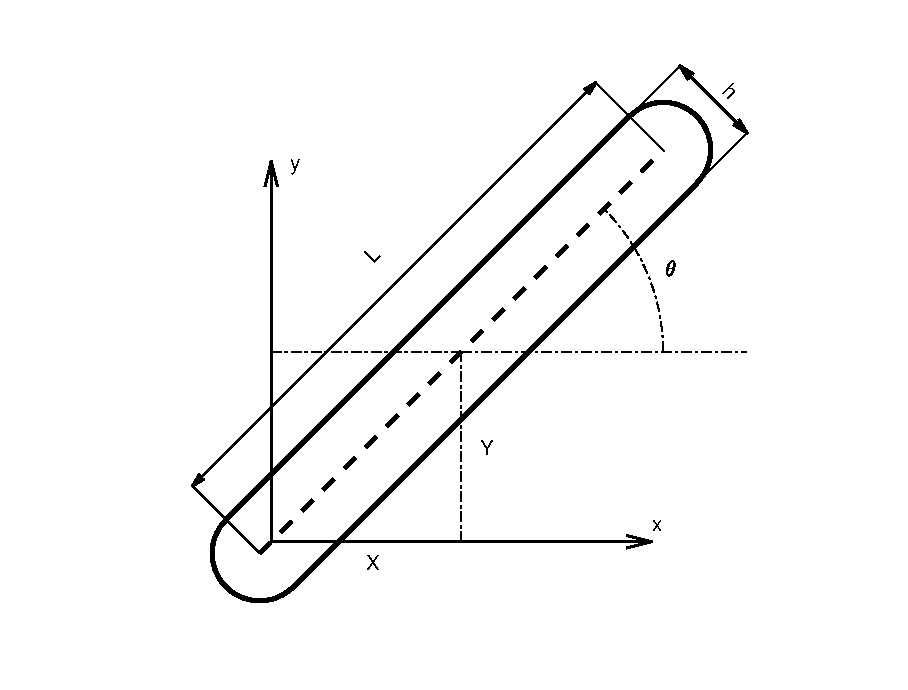
\includegraphics[width=0.5\textwidth]{images/Ch3/Scheme_bar.eps} }}%
  \subfloat[ \label{fig:s2}]{{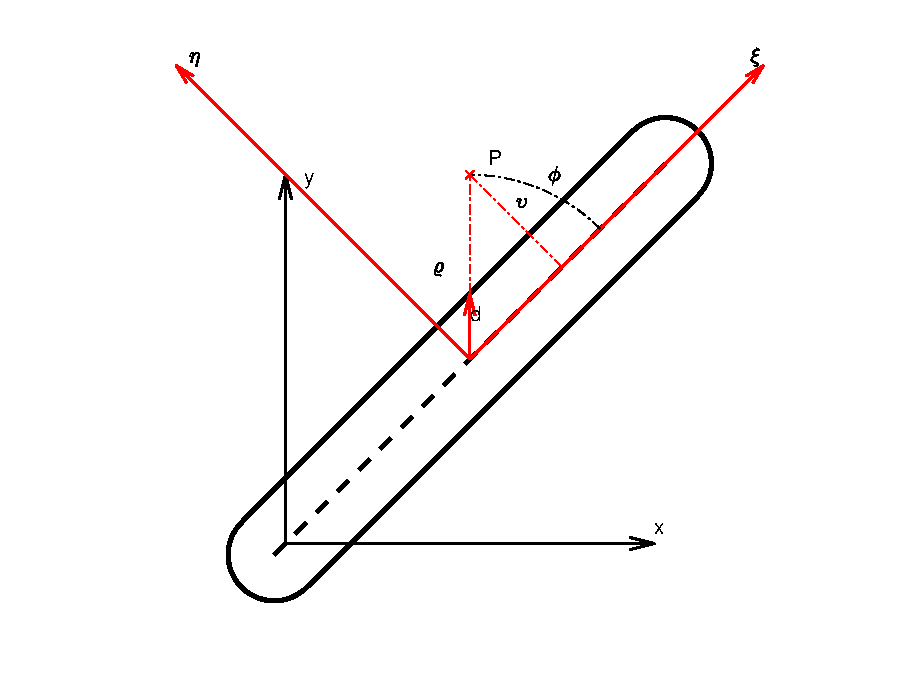
\includegraphics[width=0.5\textwidth]{images/Ch3/Scheme_bar2.eps} }}%
% Use the relevant command to insert your figure file.
% For example, with the graphicx package use
% figure caption is below the figure
\caption{Geometric primitive (i.e. basic geometric component) used for all the reviewed methods. (a) The explicit geometric parameters associated to the component are $\lbrace X,Y,L,h,\theta \rbrace$ . (b)  Plot defining the local polar coordinates  $\lbrace \varrho,\phi \rbrace^T$, the distance from the component boundary $d$, and the distance from the component middle axis $\upsilon$  } 
    % Give a unique label
\end{figure}
In order to define explicitly the contour of this component, we introduce polar coordinates $\lbrace \varrho,\phi \rbrace^T$ as defined in figure \ref{fig:s2}.
We refer to $d$ as the radial distance of the component's center $\{X,Y\}^T$ from the component boundary $\partial \omega$ that can be computed as a function of the angle $\phi$ and of the component sizes $L$ and $h$ as:
\begin{equation}
    d(\phi,L,h) = \begin{cases}
              \sqrt{\frac{h^2}{4}-\frac{L^2\sin{\phi}^2}{4}}+\frac{L}{2}|\cos{\phi}| & \text{if } \cos{\phi}^2\geq \frac{L^2}{L^2+h^2},\\
               \frac{h}{2|\sin{\phi}|} & \text{otherwise}.
          \end{cases}
\end{equation}
This piece-wise definition is at least of class $\mathbf{C}^1(\mathbb{R})$. Given a point $ \vecvar{X_g}\equiv \lbrace x,y \rbrace^T\in \mathbb{R}^2$, its polar coordinates can be defined as:
\begin{eqnarray}
    \varrho(x,y,X,Y)=\sqrt{(x-X)^2+(y-Y)^2}\\
    \phi(x,y,X,Y,\theta)  = \begin{cases}
    \arctan{\left(\frac{y-Y}{x-X}\right)}-\theta & \text{if } x\neq X,\\
    \frac{\pi}{2}\text{sign}(y-Y)-\theta & \text{if } x= X.
    \end{cases}
\end{eqnarray}
A consequence of the above definitions we have:
\begin{equation}
    \begin{array}{ccc}
   \vecvar{X_g} \in \omega \cup \partial \omega & \Leftrightarrow & d(\phi,L,h)\geq \varrho(x,y,X,Y)
    \end{array}
\end{equation}
Another way of describing the same component is by the use of the signed distance as described in Norato et al. \cite{norato2015geometry}:
\begin{equation}
\label{varsimga}
    \varsigma(\upsilon,h):=\upsilon-\frac{h}{2}
\end{equation}
where $\upsilon$ is the distance from a point $ \vecvar{X_g}\in \mathbb{R}^2$ to the component medial axis, which can be further expressed as a function of $ \vecvar{X_g}$'s polar coordinates:
\begin{equation}
\label{upsilon}
     \upsilon(\varrho,\phi,L,h)=\begin{cases}
    \sqrt{\varrho^2+\frac{L^2}{4}-\varrho L|\cos{\phi}|} & \text{if }\varrho^2\cos{\phi}^2\geq \frac{L^2}{4},\\
               \varrho|\sin{\phi}| & \text{otherwise}
    \end{cases}
\end{equation}
Accordingly,
\begin{equation}
    \begin{array}{ccc}
   \vecvar{X_g} \in \omega \cup \partial \omega & \Leftrightarrow & \varsigma(\upsilon,h)\leq 0\\
    \end{array}
\end{equation}
The structural model used during the topology optimization will then be described by $n$ components, each involving following six\footnote{additional variable $m_i$ is introduced in the geometry projection approach to make a component vanish in the same way as it is done in density based approaches.} design variables\\ $\lbrace x_i\rbrace=\lbrace X_i,Y_i,L_i,h_i,\theta_i ,m_i\rbrace^T$ . For the whole structure involving $n$ components the structural performance will thus depend on $6n$ design variables denoted as vector $\lbrace x\rbrace$:
\begin{equation}
     \lbrace x\rbrace=\left\lbrace\begin{array}{c}
          \lbrace x_1\rbrace  \\
           \lbrace x_2\rbrace  \\
           \vdots  \\
           \lbrace x_n\rbrace  \\
     \end{array}\right\rbrace
\end{equation}
Each of the reviewed methods has its own way of updating the structural model that is used to evaluate the performance of a given design. A common feature is the fact that a linear elastic-static finite element model is employed. Here a structured uniform mesh based on $dx\times dx$ solid elements in plane stress is adopted, where $dx$ is the element $x$ and $y$ size. The Poisson's ratio $\nu$ and the thickness $t$ in the out of plane direction is considered to be a constant over all the design domain $D$. The Young's modulus $E$ depends on the fact that the considered point belongs or not to $\omega$.  
A common assumption is that the Young's modulus is piece-wise uniform over each element.
For this reason, the elementary stiffness matrices $[{K}^{el}]$ are all of the same form i.e:
\begin{equation}
    [{K}^{el}]=E^{el}[{K}_0] \quad \quad  el=1,2,...,N
\end{equation}
where $E^{el}$ is the Young's modulus of the $el^{th}$ element, $[{K}_0]$ is the $8 \times 8$ stiffness matrix of a $dx\times dx$ 2D solid element in plane stress condition with thickness $t=1$ and $N$ is the total number of elements in the structural model.  
Using classic finite element theory, one can assembly the global stiffness matrix $[{K}]$:
\begin{equation}
    [{K}]=\bigoplus_{el=1}^{N} [{K}^{el}]
\end{equation}
This is used to write the static balance equation in terms of the free degrees of freedoms $\lbrace{U}\rbrace$ as:
\begin{equation}
\label{eq:10}
    [{K}]\lbrace{U}\rbrace=\lbrace{F}\rbrace
\end{equation}
where $\lbrace{F}\rbrace$ is the external loads vector. If the boundary conditions are at least isostatic and $ E^{el}\geq E_{min}>0$, then the system of equation  $[{K}]$ is non-singular and the system of equation (\ref{eq:10}) can be solved to find the displacement vector $\lbrace{U}\rbrace$.
\begin{equation}
    \lbrace{U}\rbrace=[{K}]^{-1}\lbrace{F}\rbrace
\end{equation}
In many topology optimization formulations the mass of the structure is also of interest, which is usually considered in terms of the volume fraction $V$ associated to a given structural design layout (since $V$ is proportional to the mass of a solution for a homogeneous material). To compute this volume fraction $V$ the local density $\rho^{el}$ are determined based on the design vector $\lbrace {x}\rbrace$ as will be presented in details in the next subsections for each approach.

As an example of a topology optimization formulation within this framework we provide in eq. (\ref{eq:12}) the classical formulation consisting in minimizing the compliance of the structure (i.e. maximizing its stiffness) subjected to a volume fraction constraint and design space constraints:
\begin{equation}
\label{eq:12}
    \begin{cases}
    \min_{\lbrace{x}\rbrace}{C=\lbrace{U}\rbrace^T\lbrace{F}\rbrace} \\
    s.t. \\
    V=\frac{\sum_{el=1}^{N}{\rho^{el}}}{N}\leq V_0\\
  \lbrace{l_b}\rbrace \leq \lbrace{x}\rbrace\leq\lbrace{u_b}\rbrace
    \end{cases}
\end{equation}
Where $\lbrace{l_b}\rbrace$ and $\lbrace{u_b}\rbrace$ are respectively the vectors of lower bound and upper bound for the design variables and $V_0$ is the maximum allowed volume fraction in the final solution.
\section{Moving Morphable Components (MMC) with Esartz material model}
\label{MMC}
In this section we review the moving morphable components (MMC) method (Guo et al.  \cite{guo2014doing,guo2016explicit}).
 MMC inherits from the level set method \cite{allaire2004structural} a Topology Description Function (TDF), that is positive inside the area occupied by the union of all components $\omega$, equal to zero on the boundary $\partial \omega$ of the component and negative outside the component. The TDF values are then used either to apply the XFEM \cite{wei2010study} on the boundaries of the components either to compute the element stiffness matrix using ersatz material model \cite{zhang2016new}. In this paper will focus on the application of the latter. 
 The reader must note that we made some minor modifications to the original formulation of \cite{zhang2016new}, in order to include the round ended bar components (cf. Fig. \ref{fig:sc}) with uniform thickness.
The structural topology description is obtained using a topology description function (TDF), denoted $\chi$, that satisfies following relations:
\begin{equation}
\label{eq:1}
 \begin{cases}
              \chi >0 & \text{if } \vecvar{X_g}\in \omega ,\\
               \chi =0  & \text{if } \vecvar{X_g}\in \partial\omega,\\
               \chi <0 & \text{if } \vecvar{X_g}\in D \backslash\omega.
          \end{cases}
\end{equation}
where D represents the total area of the design domain (full and voids). When more than one component is considered, the TDF of each component, denoted as $\chi_i=\chi_i(\vecvar{X_g})$, is defined $ \forall i=1,..,n$ such that:
\begin{equation}
\label{eq:2}
 \begin{cases}
              \chi_i >0 & \text{if } \vecvar{X_g}\in \omega_i ,\\
               \chi_i =0  & \text{if } \vecvar{X_g}\in \partial\omega_i,\\
               \chi_i <0 & \text{if } \vecvar{X_g}\in D \backslash\omega_i.
          \end{cases}
\end{equation}
Since $\omega=\cup_{i=1}^n{\omega_i}$ one can verify that $\chi=\max_{i}{\chi_i}$ satisfies the conditions (\ref{eq:1}).
Given a component described by the geometric variables $\lbrace X_i,Y_i,L_i,h_i,\theta_i\rbrace$ we have several choices for defining the TDF $\chi_i(\vecvar{X_g})$. Here we consider the following relationship, which has the advantage of allowing simple derivations:
\begin{equation}
\label{eq:chi}
    \chi_i=1-\left(\frac{4\upsilon_i^2}{h_i^2}\right)^\alpha \text{ with } \alpha\geq 1 
\end{equation}
Figure \ref{fig:3} illustrates the contour plot of the TDF $\chi_i$ contour of the generic component of figure \ref{fig:sc}.
\begin{figure}[!ht]
\centering
% Use the relevant command to insert your figure file.
% For example, with the graphicx package use
  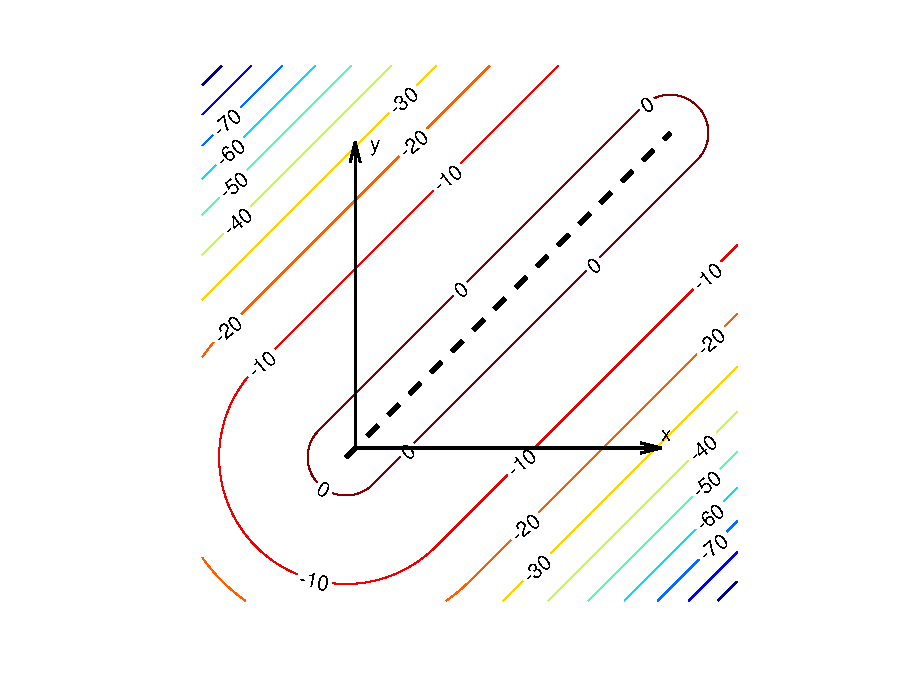
\includegraphics[width=0.5\textwidth]{images/Ch3/Chi_example.eps}
% figure caption is below the figure
\caption{$\chi(\vecvar{X_g})$ contour plot of the generic component of figure \ref{fig:sc}. We considered $\alpha=1$, $X=1$, $Y=1$, $L=3,$ $h=0.5,$ $\theta=\frac{\pi}{4}$. The domain $D$ of the plot is $[-1,2.5]\times[-1,2.5]$}
\label{fig:3}       % Give a un
\end{figure}
\begin{figure}[!ht]
\centering
% Use the relevant command to insert your figure file.
% For example, with the graphicx package use
  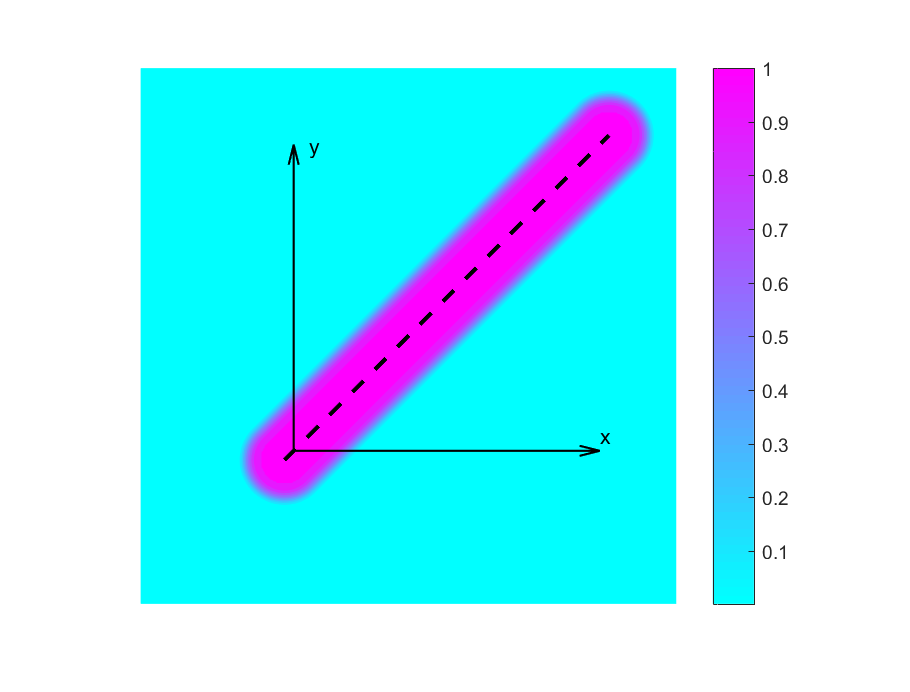
\includegraphics[width=0.5\textwidth]{images/Ch3/H_epsi_bet.eps}
% figure caption is below the figure
\caption{$H_{\epsilon}(\chi(\vecvar{X_g}))$ filled contour plot of the component in figure \ref{fig:sc}. We considered $\alpha=1$, $X=1,\ Y=1,\ L=3,\ h=0.5,\ \theta=\frac{\pi}{4}$, $\beta=0.01$, $\epsilon=0.6$. The domain $D$ of the plot is $[-1,2.5]\times[-1,2.5]$}
\label{fig:H}       % Give a unique label
\end{figure}

The presence or absence of material in the design under consideration can be obtained by the Heaviside function $H(x)$, applied to the topology description function of the union of all the components $\chi$. In order to have a regular behavior of the optimization problem responses, the Heaviside function $H(x)$ is replaced by a regularized version $H_{\epsilon}(x)$:
\begin{equation}
\label{eq:hepsi}
    H_{\epsilon}(x)=\begin{cases}
    1, & \text{if}\  x > \epsilon,\\
    \frac{3(1-\beta)}{4}\left(\frac{x}{\epsilon}-\frac{x^3}{3\epsilon^3}\right)+\frac{1+\beta}{2} & \text{if}\  -\epsilon\leq x\leq \epsilon,\\
    \beta & \text{otherwise}.
    \end{cases}
\end{equation}
Where $0<\epsilon<1$ is a parameter that controls the amplitude of the transition between the minimum value of $\beta$  ($0<\beta<<1$) and 1. The same generic component is used in figure \ref{fig:H} to plot $H_{\epsilon}(\chi(\vecvar{X_g}))$. One can observe that the smooth variation, from a value of 1 inside the component to a value of $\beta$  outside it, is localized in a small transition zone, denoted $D_g$, that can be determined using equations (\ref{eq:chi})-(\ref{eq:hepsi}):
\begin{equation}
D_g^{MMC}=\left\lbrace \vecvar{X_g}\ \mid \  \frac{h}{2}\left(1-\epsilon\right)^{\frac{1}{2\alpha}}\leq \upsilon \leq  \frac{h}{2}\left(1+\epsilon\right)^{\frac{1}{2\alpha}}\right\rbrace    
\end{equation}
The width of this transition zone is denoted by $w_g$:
\begin{equation}
    w_g^{MMC}=\frac{h}{2}\left[\left(1+\epsilon\right)^{\frac{1}{2\alpha}}-\left(1-\epsilon\right)^{\frac{1}{2\alpha}}\right]
\end{equation}
A peculiarity of MMC is that the width of the transition zone is directly proportional to the component's thickness $h$. A direct consequence is that smaller components will have faster variation between full material and voids. The effect of this behavior on the ill conditioning of the optimization problem will be investigated on numerical examples in the implementation section.

According to \cite{guo2005new}, the value of the Young's modulus in the $el^{th}$-element is considered to be:
\begin{equation}
\label{eq:EMMC}
    E^{el}=\frac{E\left(\sum_{j=1}^4(H_{\epsilon}(\chi_j^{el}))^q\right)}{4}
\end{equation}
\begin{figure*}[!ht]
\centering
    \subfloat[$\frac{ E^{el}}{E}$ \label{fig:E}]{{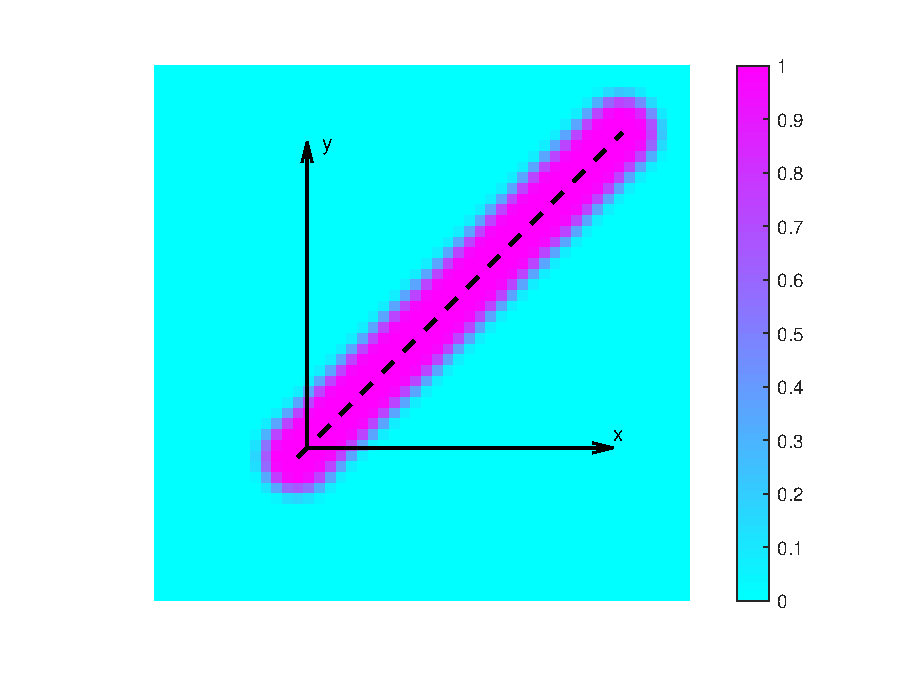
\includegraphics[width=0.45\textwidth]{images/Ch3/50x50_E.eps} }}% 
    \quad
    \subfloat[$\frac{ E^{el}}{E}$ zoom on the component boundary. \label{fig:Ez}]{{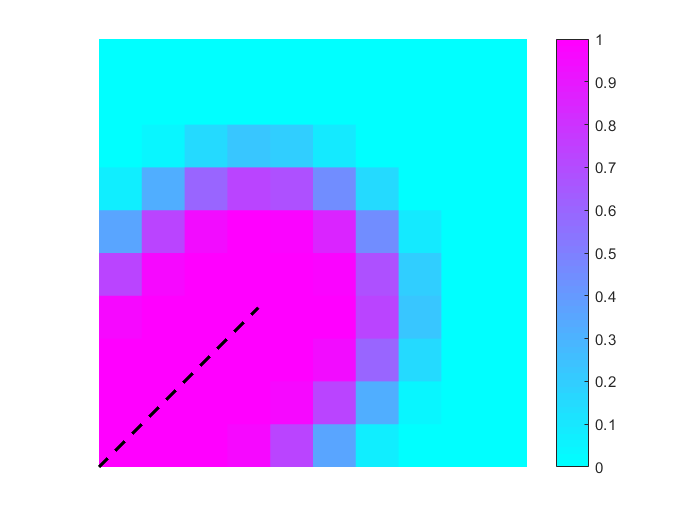
\includegraphics[width=0.45\textwidth]{images/Ch3/zoomMMCE.png} }}%
    \\
    \subfloat[$ \rho^{el}$ \label{fig:v}  ]{{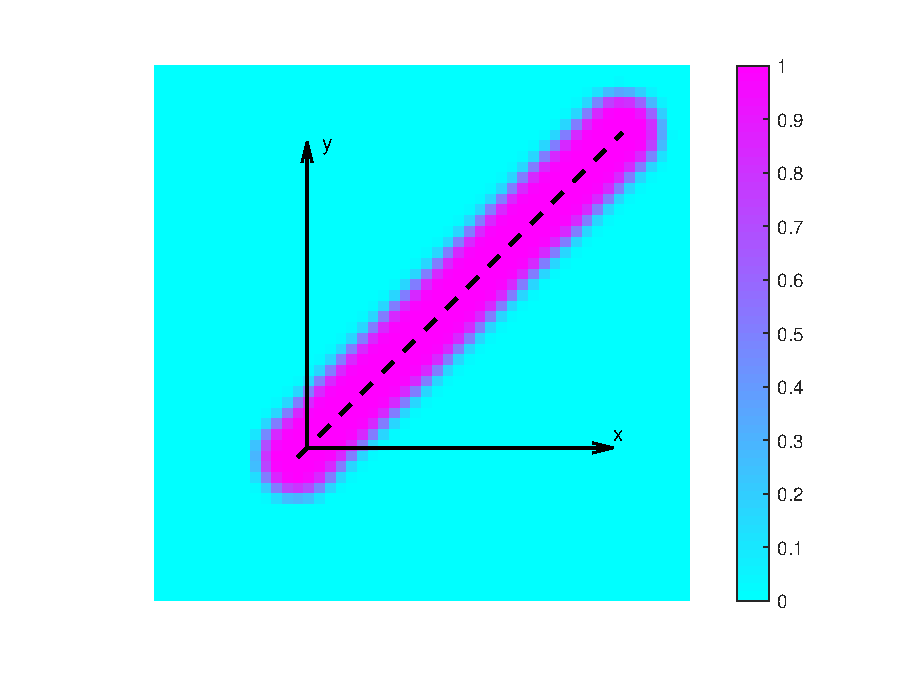
\includegraphics[width=0.45\textwidth]{images/Ch3/50x50v.eps} }}%
     \quad
        \subfloat[$ \rho^{el}$ zoom on the component boundary. \label{fig:vz}]{{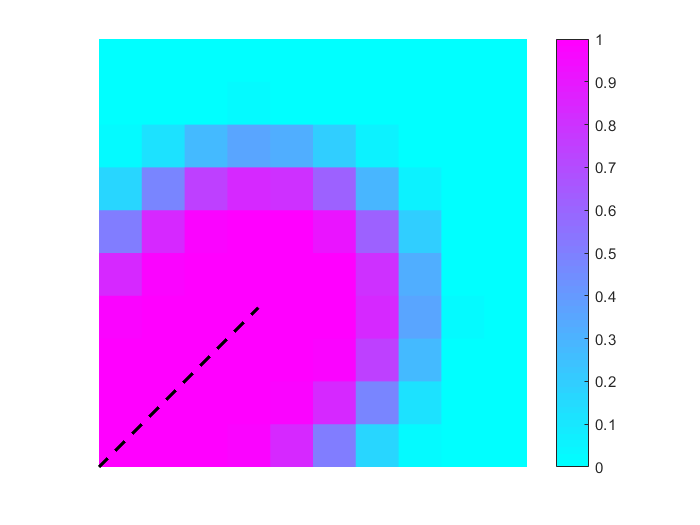
\includegraphics[width=0.45\textwidth]{images/Ch3/zoomMMC.png} }}%
    \caption{Distribution of$\frac{ E^{el}}{E}$ (a-b) and $ \rho^{el}$ (c-d)  for the generic component of figure \ref{fig:sc} and for a $50\times50$ FE mesh over the domain of $X_g$. The same parameters of figure \ref{fig:H} are also considered here with $q=2$. }%
\end{figure*}
Where $\chi_i^{el}$,$i=1,...,4$ are the values of the TDF at the four nodes of the element $el$ and $q$ is a parameters that has the role of penalization, in order to render the variation of Young's modulus even faster at the boundary of the component. In figure \ref{fig:E}, the single component example of figure \ref{fig:sc} has been used to plot the distribution of Young's modulus according to equation (\ref{eq:EMMC}) over a $50\times50$ finite element mesh. In order to obtain the local density $\rho^{el}$, which was not explicitly considered in \cite{zhang2016new}, an equivalent expression that leads to the same value of volume fraction for the same configuration is proposed here:
\begin{equation}
    \rho^{el}=\frac{\sum_{j=1}^4(H_{\epsilon}(\chi_j^{el}))}{4}
\end{equation}
In figure \ref{fig:v} the corresponding distribution of $\rho^{el}$ is also represented. Figures \ref{fig:v} and \ref{fig:E} look  very similar except for the transition on element boundary that is faster for the Young's modulus plot due to the effect of the penalization parameter $q$.
\section{Geometry Projection (GP)}
\label{GP}
In this section we review the approach proposed by Norato et al. \cite{norato2015geometry}. Geometric projection first computes the signed distance between each element central point and each component surface. The element local volume fraction is then computed by the mean of a spherical sampling window centered in the element centroid. Density and Young's modulus in the element are computed as function of the volume fraction of the sampling window that is occupied by material. The density coming from each component is unified using the maximum function or its smooth approximation \cite{kreisselmeier1980systematic}. The solution is described by the union of geometric primitives such as the one in figure \ref{fig:sc}. To update model densities the geometry projection method is employed \cite{norato2004geometry}. A circular sampling window  $\mathbf{B}_P^r$ of radius $r$ is considered around the $el^{th}$-element center $ \vecvar{X_g^{el}}$ c.f. figure \ref{fig:gp}.
The local volume fraction  $\delta^{el}$ is simply given by the fraction of the window that is filled with material:
\begin{equation}
\label{gpdef}
    \delta^{el}_i=\frac{|\mathbf{B}_P^r\cap\omega_i|}{|\mathbf{B}_P^r|}
\end{equation}
\begin{figure}[ht]
\centering
% Use the relevant command to insert your figure file.
% For example, with the graphicx package use
  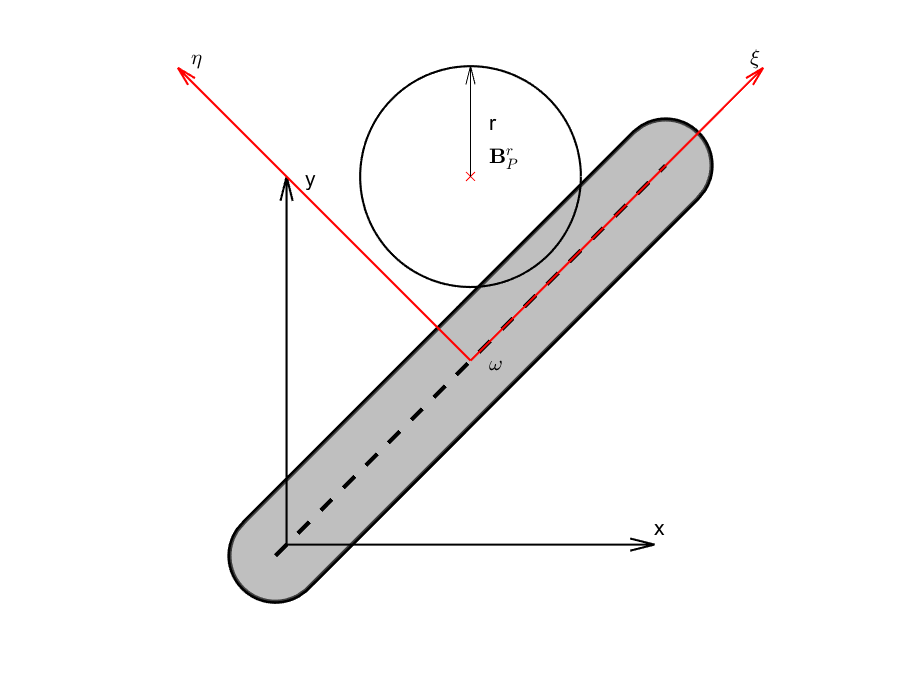
\includegraphics[width=0.55\textwidth,trim={0.8cm 0.5cm 0.5cm 0.5cm},clip]{images/Ch3/geometric_projection.eps}
% figure caption is below the figure
\caption{Basic component and notations associated to the Geometry Projection method \cite{norato2015geometry}}
\label{fig:gp}       % Give a unique label
\end{figure}
where $|\cdot|$ denotes the measure of the area. The denominator can be computed analytically as the area of the circle  $|\mathbf{B}_P^r|=\pi r^2$. The numerator of equation (\ref{gpdef}) on the other hand is more complex but can be approximately computed with the assumption that $r$ is small enough. In this case the restriction of $\partial \omega$ to the circle $\mathbf{B}_P^r$ can be considered as a straight line. As a consequence one can compute:
\begin{equation}
\label{eq:dN}
    \delta^{el}_i\approx
    \begin{cases}
    0 & \text{if}\quad\varsigma>r,\\
    \frac{1}{\pi r^2}\left[r^2\arccos{\left(\frac{\varsigma}{r}\right)}-\varsigma\sqrt{r^2-\varsigma^2}\right]& \text{if} \quad-r\leq \varsigma\leq r,\\
    1 &\quad \text{otherwise}.
    \end{cases}
\end{equation}
Where the signed distance $\varsigma$ (cf. eq. (\ref{varsimga})) is computed in the $el^{th}$ element centroid $\vecvar{X_g^{el}}$ and with respect to the $i^{th}$ component.
In order to avoid stiffness matrix singularities, the local densities are modified as follows.
\begin{equation}
    \Tilde{\delta}^{el}_i=\delta_{min}+(1-\delta_{min})\delta^{el}_i
\end{equation}
where $\delta_{min}$ is the minimum of local volume fraction to be considered in the analysis.
Moreover:
\begin{equation}
\label{eq:25}
    \hat{\delta}_i^{el}( m_i,\gamma )=\Tilde{\delta}^{el}_i m_i^\gamma  
\end{equation}
Where $m_i$ is the $i^{th}$ component mass or out of plane thickness \cite{norato2015geometry} and  $\gamma\geq1$ penalizes the intermediate value of the component's mass.
The local densities are finally computed by taking the union of all the components using a smooth approximation of the maximum function:
\begin{equation}
    \rho^{el}(\gamma_v ,\kappa)  =\Pi(\lbrace\mathbf{\hat{\delta}}^{el}(\vecvar{m},\gamma_v )\rbrace,\kappa) 
\end{equation}
where $\kappa$ is an aggregation constant and $\lbrace\hat{\delta}^{el}(\vecvar{m},\gamma_v )\rbrace$ is the vector of local density stemming from each component. Here we do not specify the form of the smooth approximation of the maximum function $\Pi$, which will be investigated in details in the section \ref{GA}. 
In order to determine the value of the Young's modulus of an element, the following equation is used which involves a second penalty parameter $\gamma_c>\gamma_v$ 
\begin{figure}[!ht]
\centering
% Use the relevant command to insert your figure file.
% For example, with the graphicx package use
  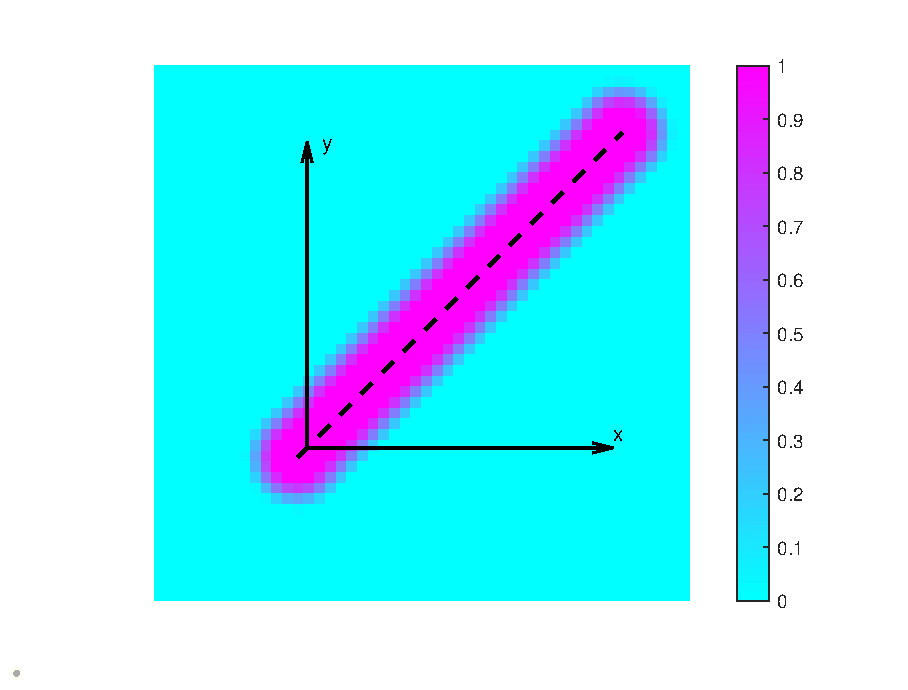
\includegraphics[width=0.45\textwidth]{images/Ch3/gpe.eps}
% figure caption is below the figure
\caption{Distribution of $ \frac{E^{el}}{E}$  for the generic component of figure \ref{fig:sc} and for a $50\times50$ mesh over the domain of $X_g$. We considered $X=1,Y=1,L=3,h=0.5,\theta=\frac{\pi}{4}, \gamma_c=3, r=0.105, \delta_{min}=10^{-6} $. Due to the choice of $m=1$  the same distribution is obtained for $\rho^{el}$.}
\label{fig:gpe}       % Give a unique label
\end{figure}
\begin{equation}
    E^{el}=\rho^{el}(\gamma_c ,\kappa)E
\end{equation}
This penalization is very similar to the one adopted by the SIMP approach and is effective in order to progressively eliminate a component with an intermediate value of $m_i$ throughout the optimization iterations \cite{norato2015geometry}. 
In figure \ref{fig:gpe}, the generic component of figure \ref{fig:sc} is considered to show the distribution of both Young's modulus and element densities over a $50\times50$ mesh. Note again that the transition zone from full material to void is concentrated on the boundary of the component:
\begin{equation}
D_g^{GP}=\left\lbrace \vecvar{X_g}\ \mid \  \frac{h}{2}-r\leq \upsilon \leq  \frac{h}{2}+r\right\rbrace    
\end{equation}
As a consequence this time the thickness of the transition zone is:
\begin{equation}
    w_g^{GP}=2r
\end{equation}
This thickness does not depend on the component size $h$. In order to achieve regular density distributions, $h$ will need to be greater or equal than $2r$. To delete inactive components, variable $m$  can still be used within the optimization algorithm.
\section{Moving Node Approach (MNA)}
\label{MNA}
Overvelde \cite{overvelde2012moving}, proposed in his master's thesis an alternative flow-inspired topology optimization approach, the Moving Node Approach (MNA). For this approach, the building blocks of a solution are defined as mass nodes. Each element's center position is recomputed with respect to a local coordinate system in each component center . Then weighting functions are directly applied to the local variable to compute the component local density contribution. In order to compute the union between the components, this time, the densities are summed. Since the sum can be greater than one, to keep the resulting density bounded from 1 an adapted procedure was proposed in \cite{overvelde2012moving} called asymptotic density. Another peculiarity of Overvelde's work was the fact of using either Finite Element Analysis or meshless method (cf. \cite{nguyen2008meshless}) for the displacement evaluation. The idea was to reduce both design variable and degrees of freedom number, using the mass nodes for both the geometric description and the solution displacement. Unfortunately in \cite{overvelde2012moving} the gain in DOFs number was compensated  by the stiffness matrix cost (both in memory and elapsed time) and by its ill conditioning where the mass nodes reached each other. The update of the finite element model is done by operating through weighting functions $w$ that are driven by the geometry of each component. In this work we considered a modified weighting function with respect to \cite{overvelde2012moving} in order to consider round ended bar components. For the mass node of figure \ref{fig:sc} one can write:
\begin{equation}
\label{eq.MNA.W}
    w(\upsilon,h,\varepsilon)=\begin{cases}
    1 & \text{if} \quad \upsilon\leq l,\\
    a_3\upsilon^3+a_2\upsilon^2+a_1\upsilon+a_0 & \text{if} \quad l<\upsilon<u,\\
    0 & \text{otherwise}.
    \end{cases}
\end{equation}
Where
\begin{eqnarray}
    l=\frac{h}{2}-\frac{\varepsilon}{2} \\  u=\frac{h}{2}+\frac{\varepsilon}{2} \\
    a_3=\frac{2}{\varepsilon^3}\\
    a_2=-\frac{3h}{\varepsilon^3}\\
     a_1=3\frac{\left(h^2-\varepsilon^2\right)}{\varepsilon^3}\\
      a_0=-\frac{(h+\varepsilon)^2(h-2\varepsilon)}{4\varepsilon^3}
\end{eqnarray}
The local density can then be computed as:
\begin{equation}
     \delta^{el}_i=m_i^\gamma w(\upsilon^{el}_i,h_i,\varepsilon_i)=m_i^\gamma w_i^{el}
\end{equation}
Where we call  $\upsilon^{el}_i$ the distance from the $el^{th}$ element centroid $\vecvar{X_g^{el}}$ to the $i^{th}$ component middle axis computed using equation (\ref{upsilon}).
To make the union of all mass nodes a smooth approximation of the maximum function is again typically employed:
\begin{equation}
    \rho^{el}=\Pi(\vecvar{\delta}_v^{el},\kappa)
\end{equation}
Finally the Young's modulus is updated using a power law:
\begin{equation}
    E^{el}=E_{min} + (E-E_{min})(\Pi(\vecvar{\delta}_c^{el},\kappa))^{p_b}
\end{equation}
Where $p_b\geq1$ is used to penalize intermediate densities.
\begin{figure*}[!ht]
\centering
    \subfloat[$\frac{ E^{el}}{E}$ \label{fig:MNAe}]{{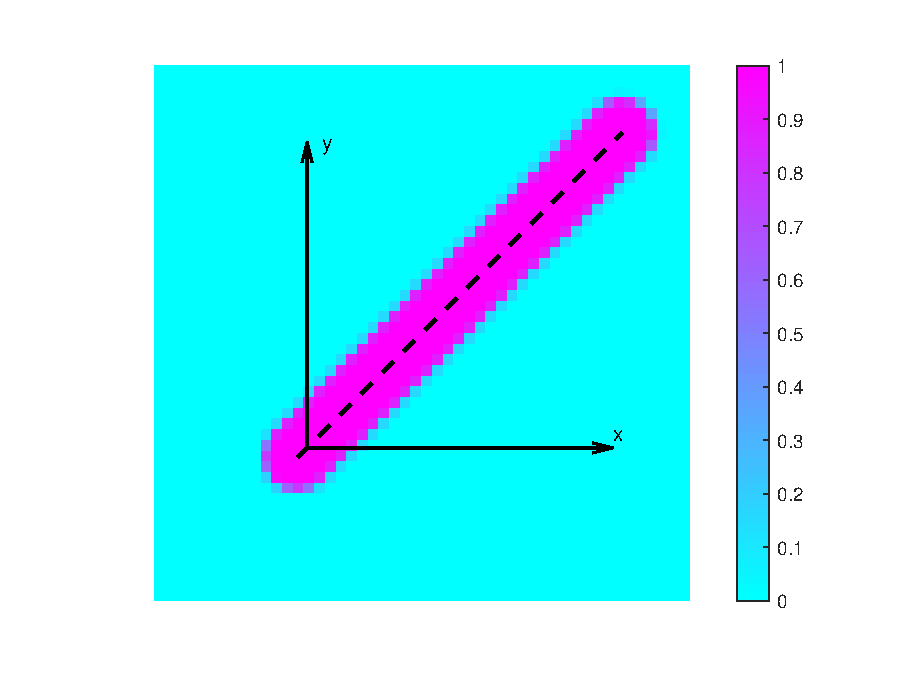
\includegraphics[width=0.45\textwidth]{images/Ch3/MNAe.eps} }}%
    \quad
    \subfloat[$\frac{ E^{el}}{E}$ zoom on the component boundary \label{fig:MNAez}]{{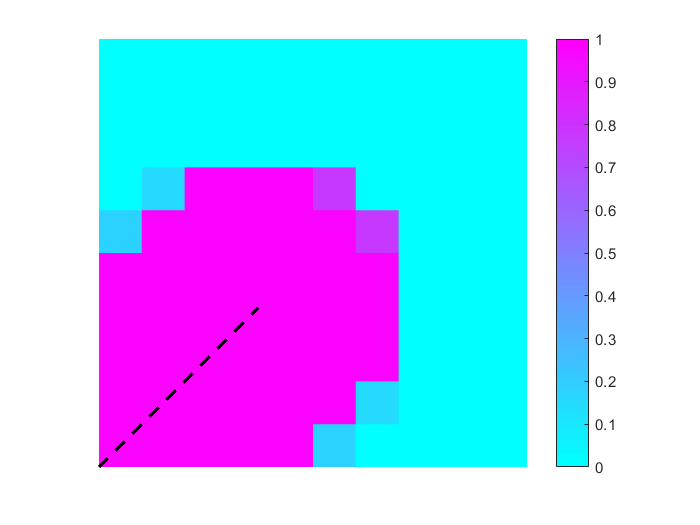
\includegraphics[width=0.45\textwidth]{images/Ch3/zoomMNAE.png} }}%
    \\
    \subfloat[$ \rho^{el}$ \label{fig:MNAv}  ]{{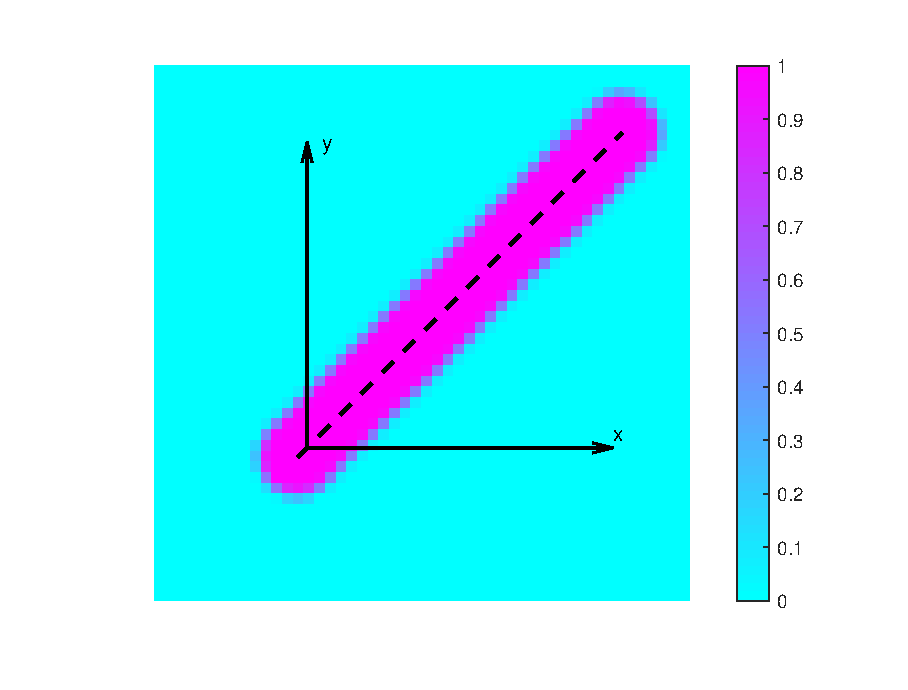
\includegraphics[width=0.45\textwidth]{images/Ch3/MNAv.eps} }}%
     \quad
        \subfloat[$ \rho^{el}$  zoom on the component boundary \label{fig:MNAvz}]{{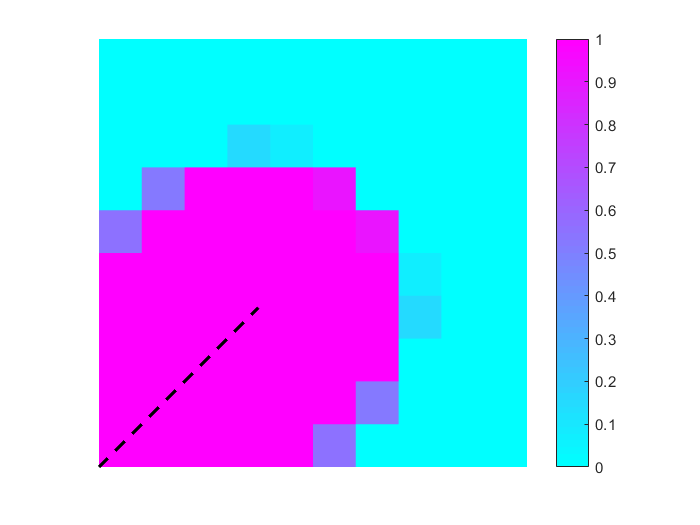
\includegraphics[width=0.45\textwidth]{images/Ch3/zoomMNA.png} }}%
    \caption{Distribution of$\frac{ E^{el}}{E}$ (a-b) and $ \rho^{el}$ (c-d)  for the generic component of figure \ref{fig:sc} and for a $50\times50$ FE mesh over the domain of $X_g$. We considered $X=1,Y=1,L=3,h=0.5,\theta=\frac{\pi}{4}, \gamma=3, \varepsilon=0.14, p_b=3 , E_{min}=10^{-6} $. }%
\end{figure*}
In figures \ref{fig:MNAe},\ref{fig:MNAv} both Young's modulus distribution and densities are considered for the same generic component and same mesh as for figures \ref{fig:E},\ref{fig:v} and \ref{fig:gpe}. Note that in this case as well the gray region is localized in the transition zone defined this time by:
\begin{equation}
D_g^{MNA}=\left\lbrace \vecvar{X_g}\ \mid \  \frac{h-\varepsilon}{2}\leq \upsilon \leq  \frac{h+\varepsilon}{2}\right\rbrace    
\end{equation}
The thickness of this transition zone is then defined as:
\begin{equation}
    w_g^{MNA}=\varepsilon
\end{equation}
This thickness is, as for Geometry Projection, independent from the component thickness $h$. On the other hand one can observe in figure \ref{fig:MNAe}, compared to Geometry Projection, the effect of the penalty $p_b>1$ that reduces the value of the Young Modulus in the transition zone. 
\section{Generalized Geometry Projection}
\label{GGP}
In this subsection we introduce the proposed Generalized Geometry Projection method as a generalization of the Geometry Projection (Bell et al. \cite{bell2012geometry}; Norato et al. \cite{norato2015geometry}; Zhang et al. \cite{zhang2016geometry}). Moreover we will show that the proposed approach can recover all the reviewed approaches in terms of relationships between the geometric configuration and finite element model update. Essentially, all reviewed approaches can be seen as a particular case of the proposed Generalized Geometry Projection method. 
Let us first formalize the general procedure that is common to all existing explicit approaches c.f. fig\ref{fig:1}.
\begin{figure}[ht]
\centering
% Use the relevant command to insert your figure file.
% For example, with the graphicx package use
  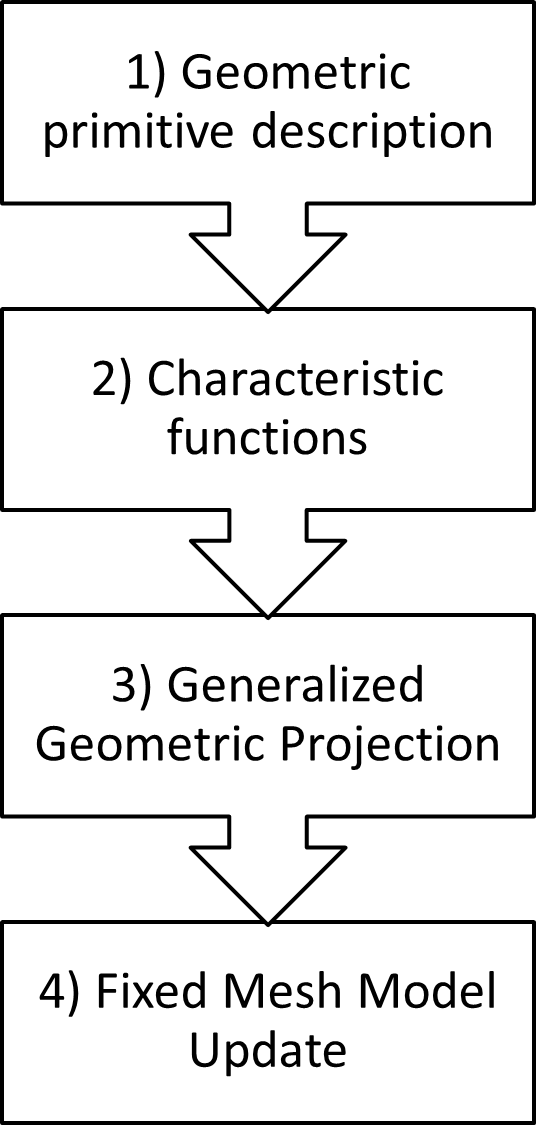
\includegraphics[width=0.25\textwidth]{images/Ch3/geometry_projection_scheme.png}
% figure caption is below the figure
\caption{General procedure employed by explicit approaches. In step 1) Geometric primitives are chosen, so that their layout, shape and sizes can be explicitly driven by the optimization procedure. In step 2) According to the geometry description characteristic functions has to be defined for each feature and for all material properties. These will be computed in each sampling window gauss points. In step 3) Generalized Geometry Projection is used to compute the value of local volume fraction for all material properties. Finally in step 4) the Finite element model is updated according to the value of each local volume fraction in each element centroid. }
\label{fig:1}       % Give a unique label
\end{figure}
The first step consists in choosing the geometric primitives, i.e. the building blocks that are going to be used to build the solution through Boolean operations. As for all reviewed approaches, round ended bar components (cf. fig. \ref{fig:sc}) in a 2D design space will be considered here as geometric primitive. Then, characteristic functions $\Upsilon$ have to be defined for each geometric primitive $i$. A characteristic function can be defined for the set of points inside the geometric primitive $\omega_i$ as:
  \begin{equation}
  \Upsilon(\vecvar{X_g},\omega_i)=\begin{cases}
        1 & \text{if} \quad \vecvar{X_g}\in \omega_i \\
        0 & \text{otherwise}.
        \end{cases}
 \end{equation}
 For implementation purpose  (in order to improve the regularity of the functions in the optimization problem), $W_i(\vecvar{X_g},\vecvar{X_i},\vecvar{r})$ should be chosen to be a regular approximation of\\ $\Upsilon(\vecvar{X_g},\omega_i)$.
 Accordingly, for the choice of a characteristic function we require here :
 \begin{equation}
\begin{cases}
     0\leq W_i(\vecvar{X_g},\vecvar{X_i},\vecvar{r})\leq 1\\
     \lim_{r\to\lambda}\left(W_i(\vecvar{X_g},\vecvar{X_i},\vecvar{r})\right)= \Upsilon(\vecvar{X_g},\omega_i)\\
      W_i(\vecvar{X_g},\vecvar{X_i},\vecvar{r})\in \mathbf{C}^{1}(\mathbb{R}^{d_g}) \\
     \end{cases}
 \end{equation}
 where $d_g$ is the dimension of the $\vecvar{X_g}$ space (in the present case $d_g=2$, since we only consider 2D problems) and  $\lambda\in\left\lbrace0,+\infty\right\rbrace$.
 The vector of hyper-parameters $\vecvar{r}$ will control the length scale of the transition of  $W_i$ between 0 and 1.  We will also require the functions $W_i$ to be non-increasing with respect to any direction that points outward of the component. For a more formal definition, we introduce the following procedure: given a point $\vecvar{X_g}\in \mathbb{R}^{d_g}$, one can find its projection on the geometric feature boundary as: $\vecvar{{X}^\star_g}=\arg \min_{\vecvar{x}\in \partial \omega_i} \|\vecvar{x}-\vecvar{X_g}\| $.
 One can then find the outward direction in $\vecvar{{X}^\star_g}$ defined as $\vecvar{n^\star}$. Finally we impose for any $\vecvar{X_g}$ that:
 \begin{equation}
     \vecvar{\frac{\partial W_i(\vecvar{X_g},\vecvar{X_i},\vecvar{r})}{\partial X_g}}^T \vecvar{n^\star}  \leq 0
 \end{equation}
 This condition avoids useless difficulties in optimization due to component border non-monotonicity.\\
 As aforementioned, a great virtue of all reviewed approaches consists in using a unique finite element model to simulate each configuration, thus avoiding re-meshing. In the proposed approach we also propose a procedure to update a given finite element model based on the configuration of the various components. In order to do so, the third step of Fig. \ref{fig:1} consists in using a procedure that transforms the continuous distribution of material represented by $W_i(\vecvar{X_g},\vecvar{X_i},\vecvar{r})$ into a piece-wise uniform distribution of Young's modulus and density inside each element of the FE mesh. The geometry projection proposed by Norato et al. \cite{norato2004geometry} is here generalized to consider several sampling window shapes.\footnote{Here we consider only $dx\times dx$ uniform meshes, but the presented framework is also valid for non-uniform and irregular meshes. Moreover, note that the sampling window shape can eventually be shaped as the finite element mesh considering a slightly different formula in the sampling window definition that we won't detail here for conciseness.}
 
 For this purpose we consider the following definition of the sampling window:
 \begin{equation}
 \begin{array}{ccc}
     \mathbf{D}(\vecvar{X_g},p,R)=\lbrace \vecvar{X}\in \mathbb{R}^{d_g} & | & \|\vecvar{X}-\vecvar{X_g}\|_{2p} \leq R  \rbrace
     \end{array}
 \end{equation}
 Next, we introduce a formulation for the local density in each element of the FE mesh that we propose in the generalized geometric projection method: 
 \begin{equation}
 \label{eq. ro}
     \delta_i^{el}(W_i,p,R)=\frac{\int_{\mathbf{D}(\vecvar{X_g^{el}},p,R)}{W_i(\vecvar{X},\vecvar{X_i},\vecvar{r})d\Omega}}{\int_{\mathbf{D}(\vecvar{X^{el}_g},p,R)}{d\Omega}}
 \end{equation}

 This formulation can be seen as a weighted volume fraction estimation over the sampling window.
 
 The evaluation of this expression can be done for example by Gauss quadrature:
 \begin{equation}
    \delta_i^{el} \approx \frac{\sum_{k=1}^{N_{gp}}{\psi_kW_{ik}}}{\sum_{k=1}^{N_{gp}}{\psi_k}}
 \end{equation}
 where $W_{ik}$ are the values of characteristic functions in Gauss point locations and $\psi_k$ are the integration weights.
 One must note that the characteristic function has not to be the same for Young's Modulus and density models. We refer to $\lbrace\delta^{el}\rbrace_v$ as the vector of local volume fractions computed in the $el^{th}$ element centroids for each component in the optimization using a density characteristic function denoted as $W^v$. In the same way we refer to   $\lbrace\delta^{el}\rbrace_c$ as the vector of local volume fraction computed in the $el^{th}$ element centroid for each component in the optimization using density characteristic function denoted as $W^c$.
 Finally the last step in the general procedure of figure \ref{fig:1} consists in updating the fixed mesh of the FE model using:
 \begin{equation}
     E^{el}=\mathbb{M}(\lbrace\delta^{el}\rbrace_c,E,E_{min},\kappa)
 \end{equation}
  \begin{equation}
     \rho^{el}=\mathbb{V}(\lbrace\delta^{el}\rbrace_v,\kappa)
 \end{equation}
 Where $\mathbb{M}$ and $\mathbb{V}$ are regular functions that link respectively the Young's modulus and local densities in each finite element to the local volume fraction values $\delta^{el}$ stemming from each geometric primitive.  \footnote{As a special case one could assemble geometric primitives before computing the local volume fractions.
 In this case the vectors of local volume fraction reduces to scalars computed that are unchanged by geometric assembly.}
 We will now show that all three reviewed approaches can be recovered as a particular case by the Generalized Geometry Projection approach.
 
 Let's consider the example of MMC with Esartz material model\footnote{This demonstration only applies to the case of $dx \times dx$ uniform meshes. The same demonstration can be easily extended to $dx \times dy$ uniform meshes simply changing sampling window definition. For the general situation of non-uniform irregular meshes, to recover the MMC formulation one should define local sampling window shapes and a more elastic numerical integration scheme based on triangulation.}.
 Let's consider $W^v=H(\chi)$,$W^c=(H(\chi))^q$, $p\to\infty$ and $R=\frac{\sqrt{3}}{2}dx$ . Let's consider Gauss-Legendre numerical integration in the sampling window, that for $p\to \infty$, is $D \equiv [-R,R]\times [-R,R]$.  We considering  $2 \times 2$ Gauss points for the numerical evaluation of the integral of equation (\ref{eq. ro}). For the function providing the element's Young's modulus we consider:
 \begin{equation}
   \mathbb{M}(\delta^{el},E,E_{min})=\lim_{p\to \infty}\delta^{el}(W^c,p,R)E_0 
 \end{equation}
 Given these assumptions we obtain the volume over a sampling window as: 
 \begin{equation}
    \lim_{p\to \infty} \int_{\mathbf{D}(\vecvar{X_g},p,\frac{\sqrt{3}}{2}dx)}{d\Omega}=\sum_{j=1}^4 \left(\frac{\sqrt{3}}{2}dx\right)^2=3 dx^2
 \end{equation}
 Furthermore, given the choice of 4 Gauss points, the integration involved in the calculation of the local volume fraction of eq. \ref{eq. ro} becomes:
 \begin{equation}
     \lim_{p\to \infty}\delta^{el}(W^c,p,R)Ñ
    \approx \frac{\frac{3}{4}dx^2\sum_{j=1}^4W^c(\mathbf{x}_j)}{3dx^2}=\frac{\sum_{j=1}^4(H(\chi(\mathbf{x}_j)))^q}{4}
  \end{equation}
 Accordingly the element's density can be expressed as:
 \begin{equation}
     \rho^{el}=\mathbb{V}(\delta^{el}(W^v,p,R),\kappa)=\lim_{p\to \infty}\delta^{el}(W^v,p,R)\approx\frac{\sum_{j=1}^4H(\chi(\mathbf{x}_j))}{4}
 \end{equation}
 These expressions for the Young's Modulus and density are the same as those employed by the MMC method with Esartz material, meaning that the Generalized Geometric Projection approach could effectively recover it. 
 
 To recover the Geometric Projection formulation, one can consider $p=1$ and a generic $R=r$. For these values the sampling window becomes a circular sampling window, i.e. $\mathbf{D}\equiv\mathbf{B_p}^r$. Moreover selecting $W_i=\Upsilon_i$ by the use of equation (\ref{eq. ro}) with the same assumption, i.e. the restriction of $\partial \omega_i$ to be considered as straight (Bell et al. \cite{bell2012geometry}; Norato et al. \cite{norato2015geometry}; Zhang et al. \cite{zhang2016geometry}) one can find the expression of the local volume fraction $\vecvar{\delta^{el}}$ .\footnote{The reader can note that the same result can also be obtained selecting $p\to \infty$, 1 Gauss point, $R=\frac{1}{2}dx$ and $W_i^{el}={\delta}_i^{el}$ of equation (\ref{eq:dN}). } In order to compute local densities we set:
  \begin{equation}
     \rho^{el}=\mathbb{V}(\vecvar{\delta}^{el},\kappa)=\Pi(\lbrace\mathbf{\hat{\delta}}^{el}( r,\gamma_v )\rbrace,\kappa) 
 \end{equation}
 And for the local Young's modulus:
  \begin{equation}
 E^{el}=\mathbb{M}(\vecvar{\delta}^{el},E,E_{min},\kappa)=\Pi(\lbrace{\hat{\delta}}^{el}(r,\gamma_c )\rbrace,\kappa) E
  \end{equation}
  Where equation (\ref{eq:25}) is used to compute $\vecvar{\hat{\delta}^{el}}$.
 
 Finally, the proposed unified approach can also recover MNA. In fact setting $W_i=m_i w(\upsilon_i,h_i,\varepsilon_i)$, $p\to\infty$ and $R=\frac{1}{2}$ and using numerical integration for the integrals in equation (\ref{eq. ro}) with just a single Gauss point one gets:
 \begin{equation}
     \delta_i^{el}\approx W_i=m_i^\gamma w_i^{el}
 \end{equation}
 This time for the local densities:
 \begin{equation}
    \mathbb{V}(\vecvar{\delta^{el}},\kappa)=\Pi(\lbrace\mathbf{{\delta}}^{el}\rbrace_v,\kappa) 
 \end{equation}
 And for the Young's modulus:
  \begin{equation}
    \mathbb{M}(\vecvar{\delta^{el}},\kappa)=E_{min}+(E-E_{min})\Pi\left(\lbrace\mathbf{{\delta}}^{el}\rbrace_c,\kappa\right)^{p_b}
 \end{equation}
  A summary of the parameters to be used in the proposed Generalized Geometric Projection approach to recover all of the three reviewed methods is provided in table \ref{tab:1}.\\
\begin{table*}[!h]
% table caption is above the table
\caption{Choice to be made to recover all other approaches using Generalized Geometric Projection }
\label{tab:1}       % Give a unique label
\centering
% For LaTeX tables use
\begin{tabular}{llll}
\hline\noalign{\smallskip}
Method & MMC & GP & MNA \\
\noalign{\smallskip}\hline\noalign{\smallskip}
$W^c$ & $H_{\epsilon}(\chi^{el})^q$ & $\Tilde{\delta}_i^{el} m_i^{\gamma_c}$&  $m_i^{\gamma_c} w^{el}_i$\\
$W^v$ &$H_{\epsilon}(\chi^{el})$  & $\Tilde{\delta}_i^{el} m_i^{\gamma_v}$&  $m_i^{\gamma_v} w^{el}_i$\\
$p$ &  $\infty$&$\infty$&$\infty$\\
$R$ & $\frac{\sqrt{3}}{2}dx$&  $\frac{1}{2}dx$&  $\frac{1}{2}dx$\\
$N_{GP}$ &  $4$&$1$&$1$\\
$\mathbb{V}$ & $\frac{\sum_{j=1}^4 H_{\epsilon}(\chi_j^{el})}{4}$ & $\Pi(\vecvar{\hat{\delta}^{el}}_v,\kappa)$ & $\Pi(\vecvar{{\delta}^{el}}_v,\kappa)$ \\
$\mathbb{M}$ & $\frac{\sum_{j=1}^4 (H_{\epsilon}(\chi_j^{el}))^q}{4}$ & $\Pi(\vecvar{\hat{\delta}^{el}}_c,\kappa)E$ & $E_{min}+(E-E_{min})\Pi(\vecvar{{\delta}^{el}}_c,\kappa)^{p_b}$ \\
\noalign{\smallskip}\hline
\end{tabular}
\end{table*}
Note that for the proposed GGP approach, it is not only possible to recover existing strategies, but it is also possible to adapt an existing technique by changing only $R$ and $N_{GP}$., in order to potentially improve the analysis and optimization behavior.
  In this paper we will then refer to: Adapted Moving Morphable Components method (AMMC), Adapted Geometry Projection (AGP) and to Adapted Moving Node Approach (AMNA), when using respectively MMC, GP or MNA parameters in table \ref{tab:1} with the only exceptions of  number of Gauss points in each sampling window $N_{GP}$ and of the sampling window size $R$. In figure \ref{fig:MNAv234} the Adapted Moving Node Approach is applied to the same example considered in figure \ref{fig:sc} to compute $\rho^{el}$ distribution on a uniform $50\times 50$ mesh and investigates the variation of both $R$ and $N_{GP}$.
  In this case we considered MNA characteristic function with a relatively small $\varepsilon$. When just one Gauss point is employed for the numerical integration, $R$ has no effect on the final $\rho^{el}$ distribution. One can observe that increasing $N_{GP}$ smoothens the $\rho^{el}$ variations around the bar ends. On the other hand increasing the value of $R$ smoothens the variation between full and voids elements. These effects are important from the simulation and optimization point of view as will be pointed out in the implementation section.

\begin{figure*}[!ht]
\centering
    \subfloat[$R=\frac{1}{2}dx$ , $N_{GP}=1$]{{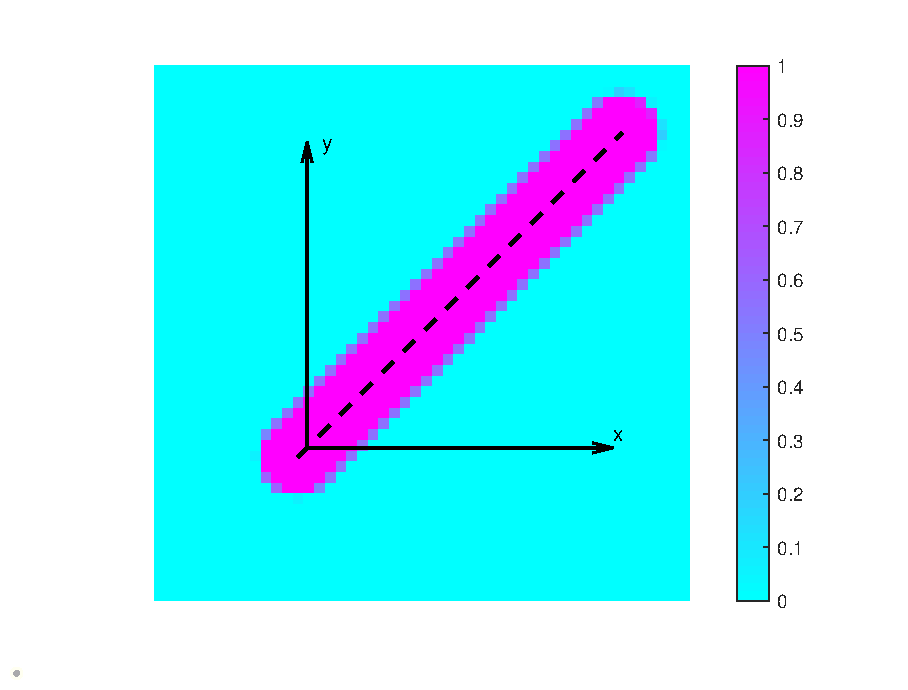
\includegraphics[width=0.4\textwidth]{images/Ch3/MNAv1.eps} }}%
    \quad
    \subfloat[$R=dx$ , $N_{GP}=1$]{{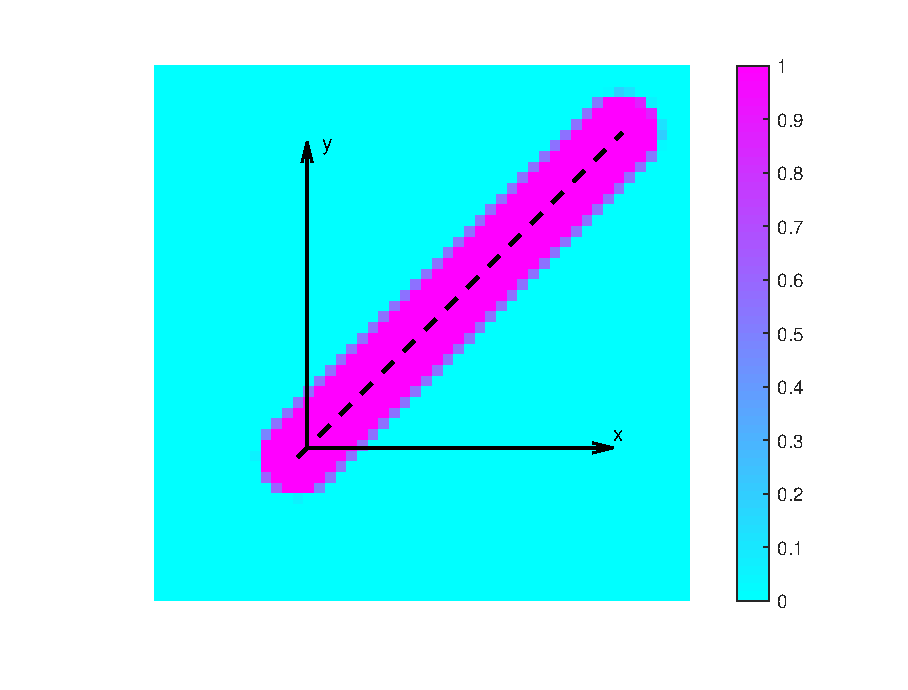
\includegraphics[width=0.4\textwidth]{images/Ch3/MNAv1R1.eps} }}%
    \\
    \subfloat[$R=\frac{1}{2}dx$ , $N_{GP}=4$]{{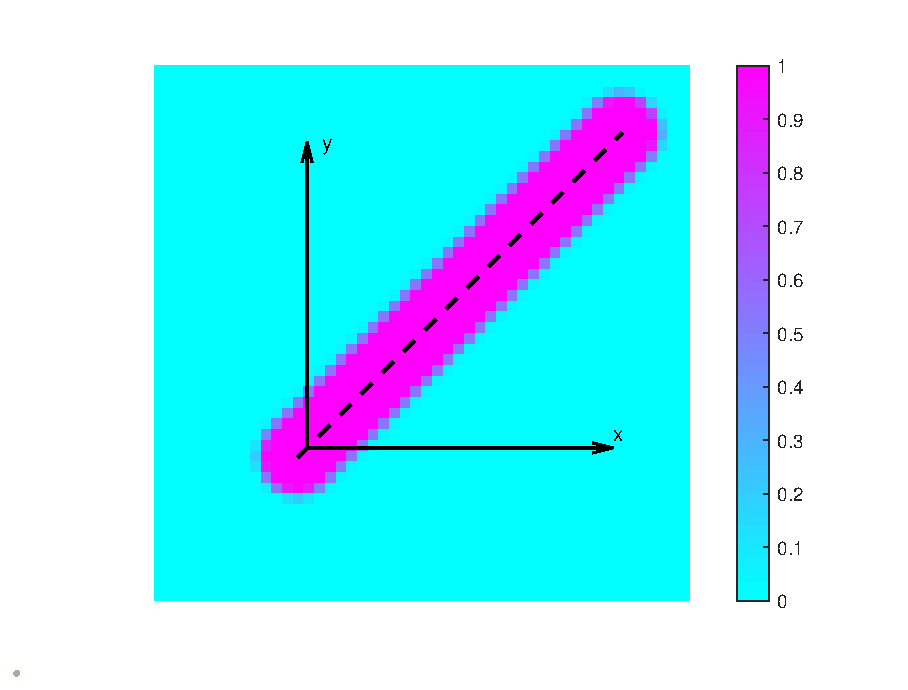
\includegraphics[width=0.4\textwidth]{images/Ch3/MNAv2.eps} }}%
    \quad
    \subfloat[$R=dx$ , $N_{GP}=4$]{{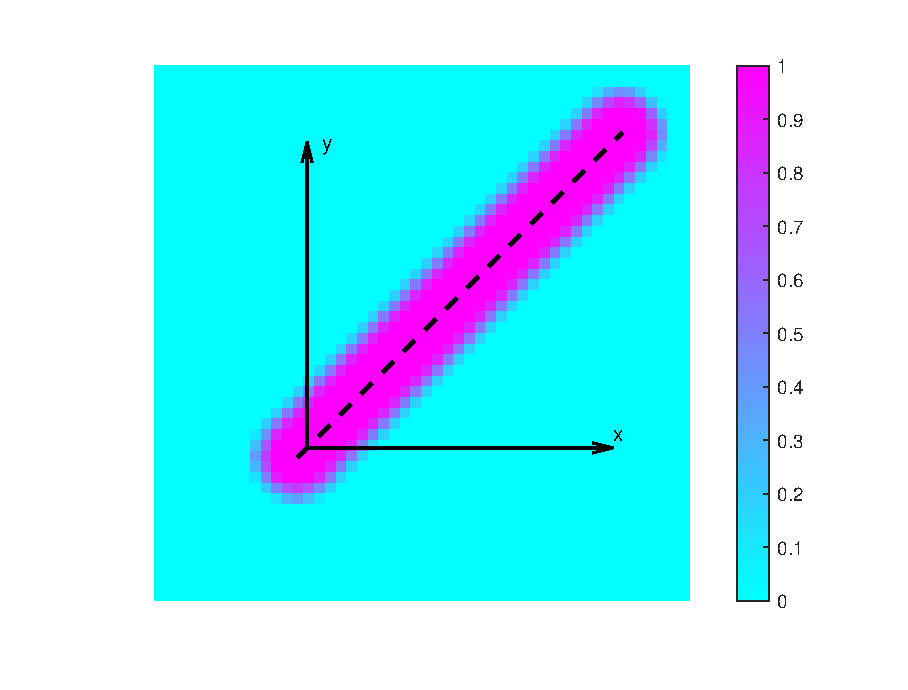
\includegraphics[width=0.4\textwidth]{images/Ch3/MNAv2R1.eps} }}%
    \\
    \subfloat[$R=\frac{1}{2}dx$ , $N_{GP}=9$]{{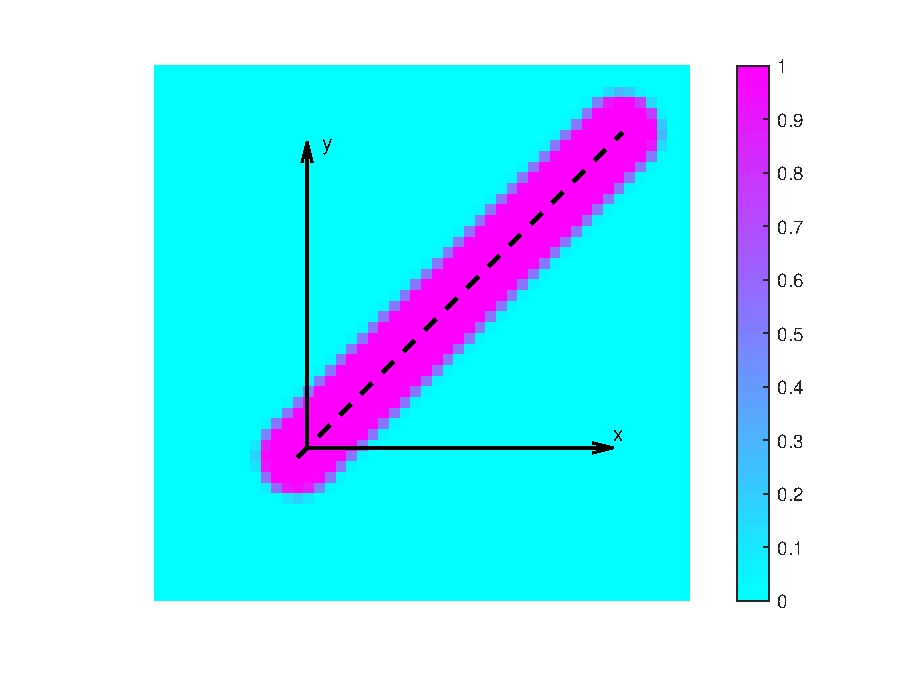
\includegraphics[width=0.4\textwidth]{images/Ch3/MNAv3.eps} }}%
    \quad
    \subfloat[$R=dx$ , $N_{GP}=9$]{{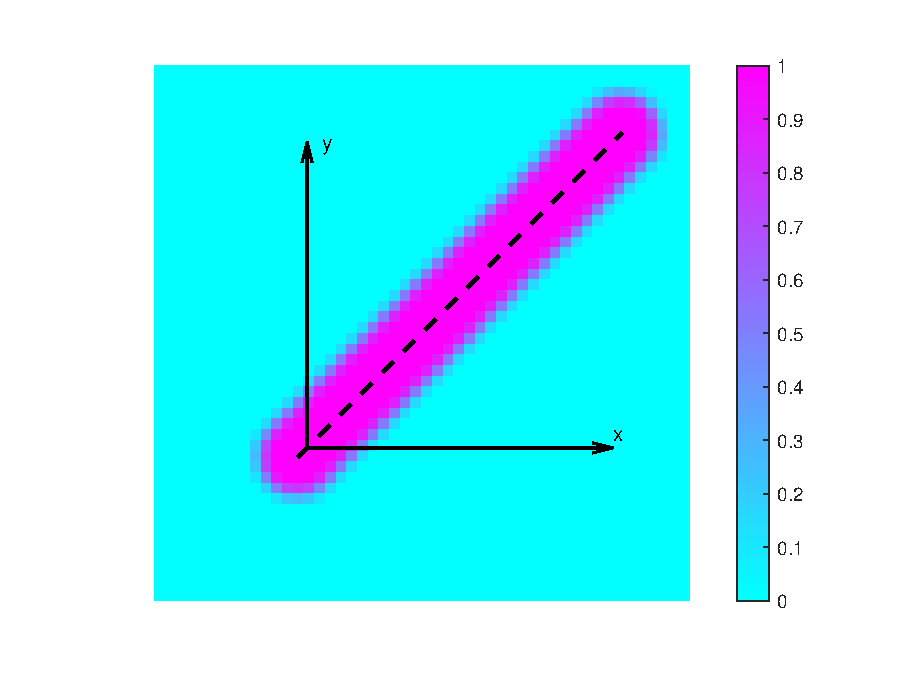
\includegraphics[width=0.4\textwidth]{images/Ch3/MNAv3R1.eps} }}%
    \caption{Distribution of $ \rho^{el}$ for the generic component of figure \ref{fig:sc} and for a $50\times50$ mesh over the domain of $X_g$ for carrying number of Gauss points. We considered MNA characteristic functions $X=1,Y=1,L=3,h=0.5,\theta=\frac{\pi}{4}, \gamma=3, \varepsilon=0.07$ as for MNA. The mesh size $dx$ along the x direction was considered as $dx=0.07$. }%
    \label{fig:MNAv234}%
\end{figure*}
\section{Geometric assembly}
\label{GA}
As discussed in the previous subsections, several approaches were reviewed for making the union or the assembly of geometric primitives.
In the first place, we want to point out, as it was done by Norato et al. \cite{norato2015geometry}, that the assembly of 2D components can be seen as a merging operation (the component's thickness doesn't change at the intersection) or as an overlapping operation (the component thickness is summed).
In the first case one is interested in determining the union of the geometry produced by each component, while in the second case the geometry are simply overlapped in the out of plane direction. Since the stiffness matrix of each finite element is proportional to both the Young's modulus and the out of plane thickness, the local volume fraction of each component could be simply summed up in this case and used to determine an equivalent Young's Modulus that takes into account both the effect of material and out of plane thickness.
This ambiguity does not exist in 3D topology optimization where the only possibility to make the assembly is the merging strategy. The rest of this paragraph will then focus on the strategy that can be adopted to merge component's geometries.
Firstly one can observe that depending on the considered approach, the assembly is carried out either on local volume fractions or more indirectly through topology description functions (TDF) as in Zhang et al. \cite{zhang2016new}. 
 \footnote{The characteristic function of the union of sets can be easily computed as the maximum of the characteristic functions of each set. The same can be stated for TDFs.}
 In \cite{zhang2017comprehensive} a comprehensive study of application of Boolean operations is reviewed for implicit geometry description (R-functions or TDF).
 In this context we first want to consider the case when the geometric assembly is applied at the level of the density field. The main advantage of this case consists in being able to treat the local volume fraction coming from each component projection as a pseudo-logical value. In fact let's consider an input vector $\lbrace{z}\rbrace \in \{0,1\}^n$. In order to make the logic union of all the entry vectors, one can consider either one of the following approaches:
 \begin{eqnarray}
 \Pi_a(\vecvar{z})=\min\left(1,\sum_{i=1}^n{z_i}\right)\\
 \Pi_b(\vecvar{z})=1-\prod_{i=1}^n{\left(1-z_i\right)}\\
 \Pi_{max}(\vecvar{z})=\max_i{z_i}
 \end{eqnarray}
For a logical entry vector  $\lbrace{z}\rbrace\in \{0,1\}^n$, $\Pi_a(\vecvar{z})=\Pi_b(\vecvar{z})=  \Pi_{max}(\vecvar{z})$. On the other hand when $\lbrace \mathbf{z}\rbrace \in ]0,1[^n$ then
$\Pi_a(\vecvar{z})\neq\Pi_b(\vecvar{z}) \neq  \Pi_{max}(\vecvar{z})$. The asymptotic density operator $\Pi_a(\vecvar{z})$ first makes an overlap of the component's density and then saturate the result to 1. This approach was employed in the master thesis of Overvelde \cite{overvelde2012moving}. The minimum between 1 and the value of the sum can be realized by a regular saturation function that is detailed later in this paragraph. The Boolean operator $\Pi_b(\vecvar{z})$ can be recognized as the one employed by the MMB \cite{hoang2017topology} approach in order to make the union of bar components. For the third approach, since the maximum is an irregular function, in the literature it is often replaced with its regular approximations. In the context of topology optimization we can cite the p-norm and the p-mean \cite{duysinx1998new}, the Kreisselmeier–Steinhauser (KS) functional \cite{kreisselmeier1980systematic} and the more recent induced approaches \cite{kennedy2015improved}.Often these approximations are employed in structural optimization with stress constraints in order to reduce the number of constraints in the optimization problem.
Here we review these methods and some important properties relative to the maximum operator. Given an input vector $\lbrace \mathbf{z}\rbrace \in \mathbb{R}^n$, and the constant of aggregation $\kappa\in\mathbb{R}^+ $, the smooth approximation $\Pi$ of the maximum operator is defined as:
$\Pi: \left(\mathbb{R}^n,\mathbb{R}^{+} \right) \rightarrow \mathbb{R}\  | \  (\lbrace \mathbf{z}\rbrace,\kappa) \rightarrow \Pi(\lbrace \mathbf{z}\rbrace,\kappa)$  and
\begin{equation}
\label{eq:lp}
    \lim_{\kappa\to\infty}\Pi(\lbrace \mathbf{z}\rbrace,\kappa)=\max(\lbrace \mathbf{z}\rbrace)=z_{max}
\end{equation}
Let’s consider the p-norm $\Pi_{pm}$ and the p-mean $\Pi_{pn}$ \cite{duysinx1998new}.
For these approaches one can make the assumption that an input vector $\lbrace \mathbf{z}\rbrace$ has non negative components, thus:
\begin{equation}
    \Pi_{pm}(\lbrace \mathbf{z}\rbrace,\kappa)=\left(\frac{1}{n}\sum_{j=1}^n z_j^{\kappa}\right)^{\frac{1}{\kappa}}\leq z_{max} <\left(\sum_{j=1}^n z_j^{\kappa}\right)^{\frac{1}{\kappa}}=\Pi_{pn}(\lbrace \mathbf{z}\rbrace,\kappa)
\end{equation}
One can also have negative inputs but a double correction has to be made in order to have all non-negative inputs when elevating to the power $\kappa$. For instance one can choose a positive value $z_p$ so that $z_j+z_p>0\  \forall j=1,2,...,n$ with this modification one can compute: 
\begin{eqnarray}
   \Pi_{pm}^{p}(\lbrace \mathbf{z}\rbrace,\kappa,z_p)=\left(\frac{1}{n}\sum_{j=1}^n (z_j+z_p)^{\kappa}\right)^{\frac{1}{\kappa}}-z_p  \\
   \Pi_{pn}^{p}(\lbrace \mathbf{z}\rbrace,\kappa,z_p)=\left(\sum_{j=1}^n (z_j+z_p)^{\kappa}\right)^{\frac{1}{\kappa}}-z_p
\end{eqnarray}

We will also review here both lower bound KS function $\Pi^l_{KS}$ and the KS function $\Pi_{KS}$ \cite{kreisselmeier1980systematic}:
\begin{equation}
    \Pi^l_{KS}(\lbrace \mathbf{z}\rbrace,\kappa)=\frac{1}{\kappa}\log{\left(\frac{1}{n}\sum_{j=1}^n e^{\kappa z_j}\right)}\leq z_{max} <\frac{1}{\kappa}\log{\left(\sum_{j=1}^n e^{\kappa z_j}\right)}=\Pi_{KS}(\lbrace \mathbf{z}\rbrace,\kappa)
\end{equation}
Finally we considered also the induced exponential $\Pi_{IE}$ \cite{kennedy2015improved}:
\begin{equation}
     \Pi_{IE}(\lbrace \mathbf{z}\rbrace,\kappa)=\frac{\sum_{j=1}^n z_j e^{\kappa z_j}}{\sum_{j=1}^n e^{\kappa z_j}}\leq z_{max}
\end{equation}
In figure \ref{fig:pbb},\ref{fig:pb}, \ref{fig:kb} and \ref{fig:ib} all reviewed operators are applied to the vector $\lbrace\mathbf{z}\rbrace=\{x,10xe^{1-10x},4x(1-x)\}$ for $x\in[0,1]$.
\begin{figure}[!ht]
\centering
% Use the relevant command to insert your figure file.
% For example, with the graphicx package use
  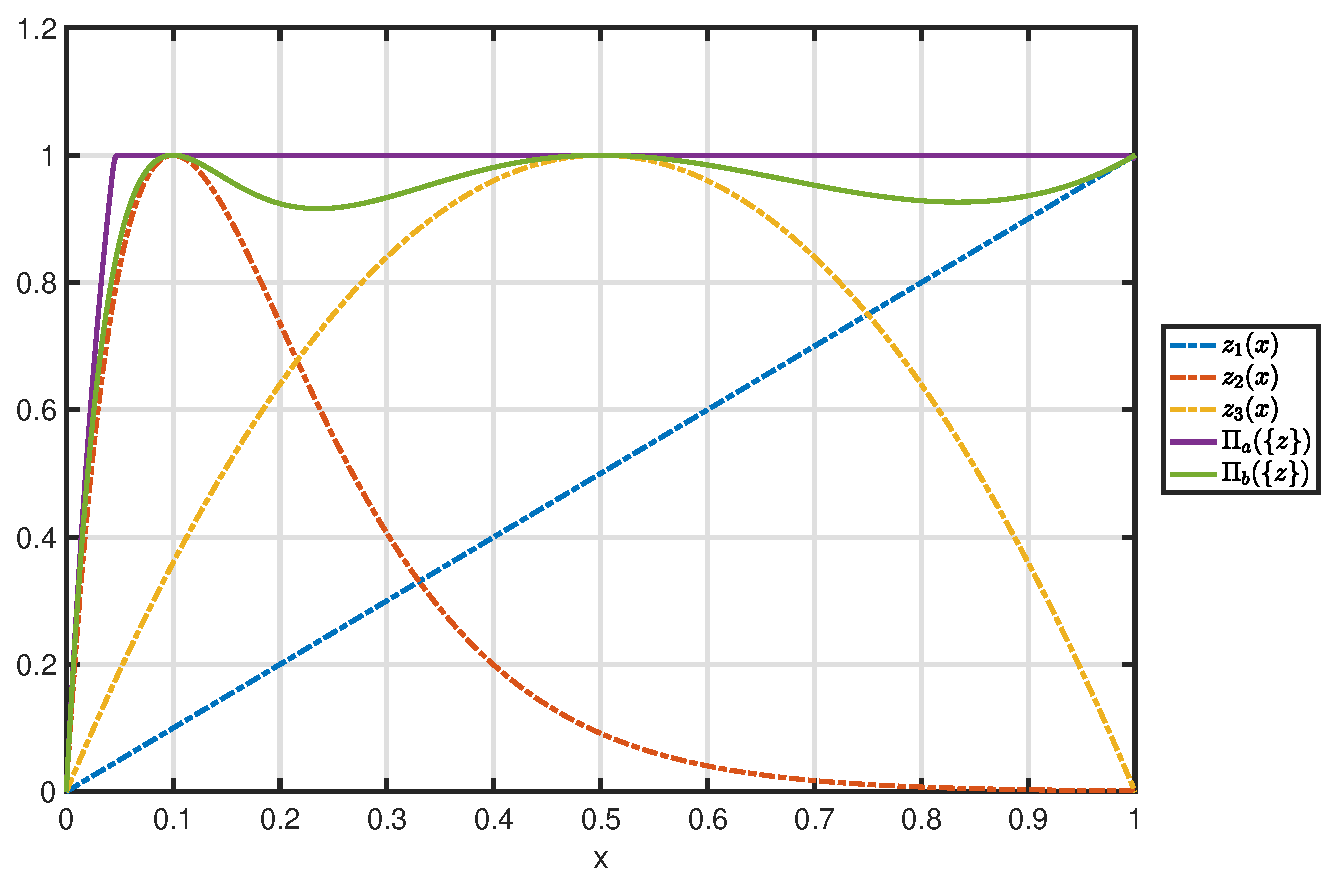
\includegraphics[width=0.5\textwidth]{images/Ch3/pbbench.eps}
% figure caption is below the figure
\caption{Application of asymptotic density operator $\Pi_{a}$ and of  Boolean operator $\Pi_{b}$ to the vector $\mathbf{z}$ of 3 variables,$z_1(x)=x,z_2(x)=10xe^{1-10x},z_3(x)=4x(1-x)$. The minimum function necessary to carry out the evaluation of $\Pi_{a}$ is replaced by the regular approximation of the saturation function of equation (\ref{eq:st}). }
\label{fig:pbb}       % Give a unique label
\end{figure}
\begin{figure}[!ht]
\centering
% Use the relevant command to insert your figure file.
% For example, with the graphicx package use
  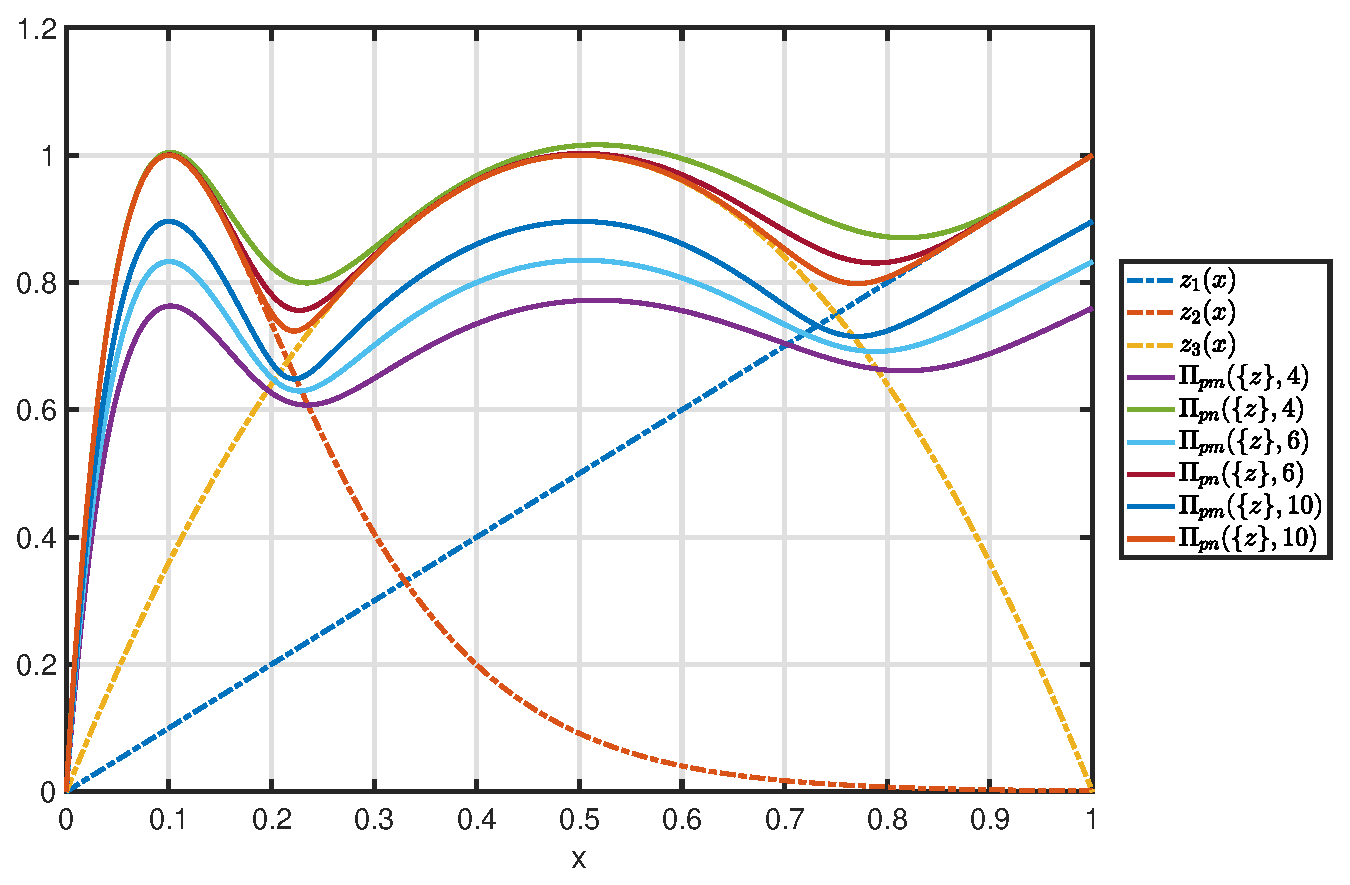
\includegraphics[width=0.5\textwidth]{images/Ch3/pmpnbench.eps}
% figure caption is below the figure
\caption{Application of p-norm $\Pi_{pn}$ and p-mean $\Pi_{pm}$ operator for $\kappa=4,6,10$ to the vector $\mathbf{z}$ of 3 variables,$z_1(x)=x,z_2(x)=10xe^{1-10x},z_3(x)=4x(1-x)$.}
\label{fig:pb}       % Give a unique label
\end{figure}
\begin{figure}[!ht]
\centering
% Use the relevant command to insert your figure file.
% For example, with the graphicx package use
  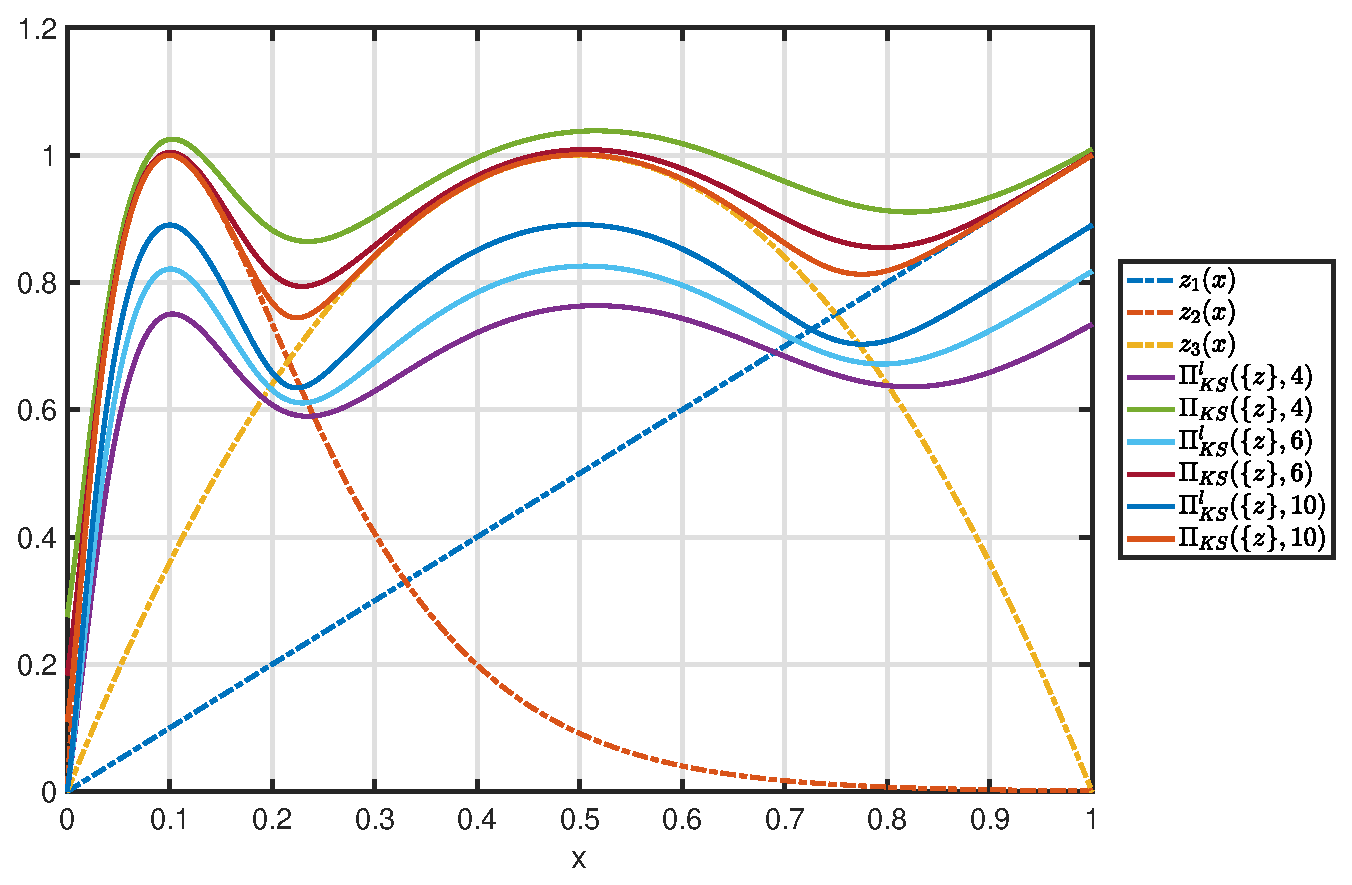
\includegraphics[width=0.5\textwidth]{images/Ch3/KSbench.eps}
% figure caption is below the figure
\caption{Application of KS $\Pi_{KS}$ and lower bound KS $\Pi_{KS}^l$ function for $\kappa=4,6,10$ to the vector $\mathbf{z}$ of 3 variables, $z_1(x)=x,z_2(x)=10xe^{1-10x},z_3(x)=4x(1-x)$.}
\label{fig:kb}       % Give a unique label
\end{figure}
\begin{figure}[!ht]
\centering
% Use the relevant command to insert your figure file.
% For example, with the graphicx package use
  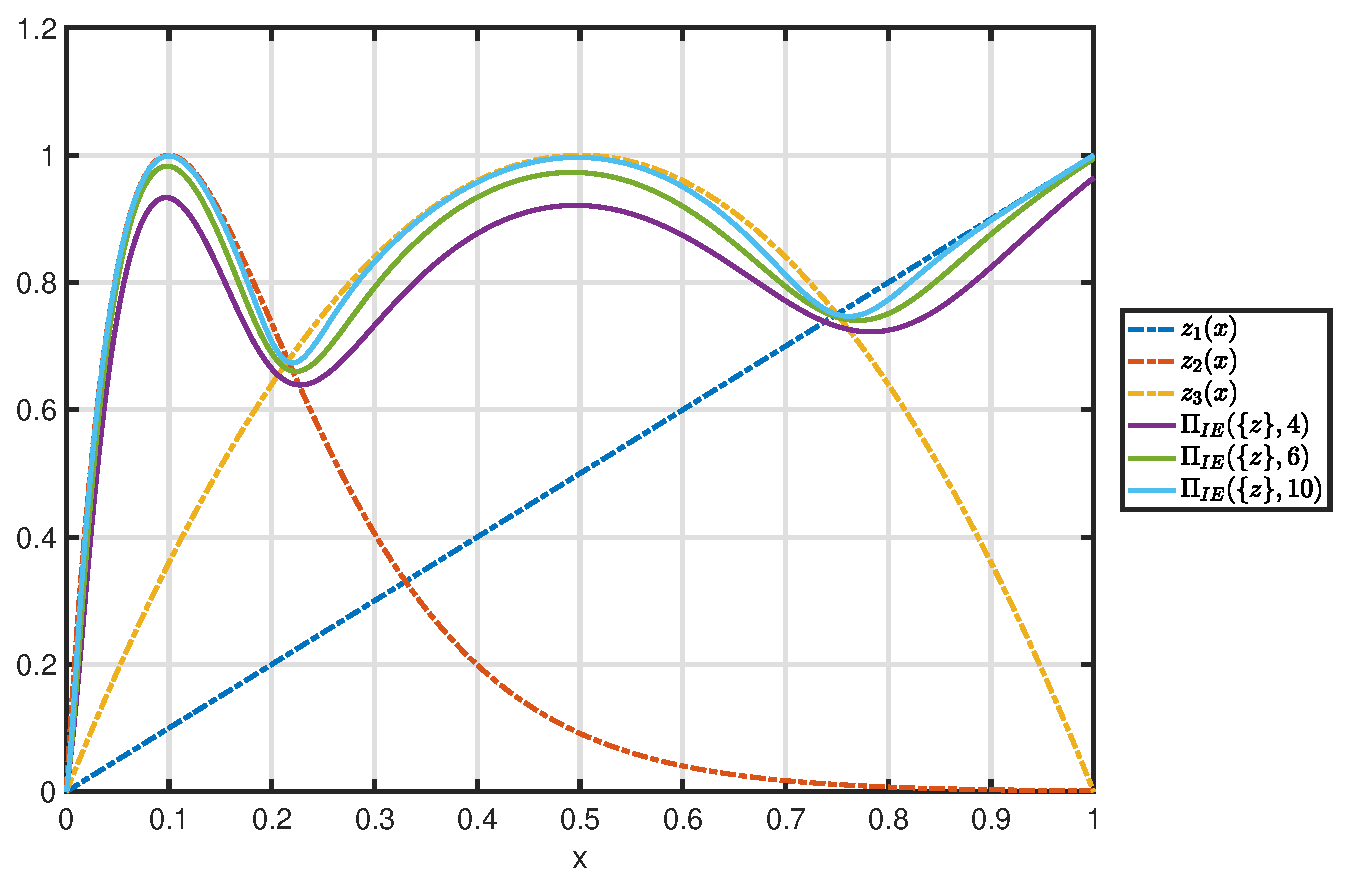
\includegraphics[width=0.5\textwidth]{images/Ch3/iebench.eps}
% figure caption is below the figure
\caption{Application of induced exponential aggregation function $\Pi_{IE}$ for $\kappa=4,6,10$ to the vector $\mathbf{z}$ of 3 variables,$z_1(x)=x,z_2(x)=10xe^{1-10x},z_3(x)=4x(1-x)$.}
\label{fig:ib}       % Give a unique label
\end{figure}
 A first important remark is that p-mean, lower bound KS function and induced exponential operator are always less than or equal to the maximum. The equality being true in the case of uniform value for the entry vector i.e.:
\begin{equation}
    \Pi_{pm}(\lbrace \mathbf{z}\rbrace,\kappa)=\Pi_{KS}^l(\lbrace \mathbf{z}\rbrace,\kappa)=\Pi_{IE}(\lbrace \mathbf{z}\rbrace,\kappa)=z_{max} \Leftrightarrow z_1=z_2=...=z_n=z_{max} 
\end{equation}
On the other hand Boolean, asymptotic density, p-norm and KS functions are always strictly greater than the maximum function.
A second remark is that most reviewed approaches ( with the exceptions of the asymptotic density and the Boolean operator ) produce regular approximations of the maximum function and that by increasing the value of the aggregation constant $\kappa$, all approaches tend to recover the maximum function as requested in equation (\ref{eq:lp}). At the same time high values of $\kappa$ reduces the smoothness of the approximated function. A third important remark is that the absolute value of the discrepancy between  $z_{max}$ and the approximation are maximized in the following way depending on the aggregation approach employed:
\begin{itemize}
    \item For p-norm and KS function the worst accuracy corresponds to a uniform entry vector $\mathbf{z}$.
    \item For p-mean and lower bound KS function the worst accuracy corresponds to a vector $\mathbf{z}$ so that: $z_i=u_b \Leftrightarrow i=i_{max}$ and $z_i=l_b \forall i\neq i_{max}$. Where $u_b$ and $l_b$ are respectively the lower and the upper bound of entry vector components.
    \item For the induced exponential operator the worst accuracy is reached in intermediate cases
\end{itemize}
Coming back to the application of these functions to the component assembly, one should consider the following implications:
\begin{itemize}
\item Asymptotic density and Boolean operator are thought to be used on pseudo-logical input, i.e. $\in [0,1]$. They could also be adopted for TDF but some re-scaling of the input should be adopted to have a meaningful behavior of both operators. 
\item If the assembly is made on TDFs as in Zhang et al. \cite{zhang2016new}, p-norm and p-mean cannot be employed as they are, but they need to be modified in order to avoid a negative value of the argument of the power.
\item When considering TDF applications, one is free to use both KS functions and the induced exponential operator without particular numerical difficulties.
\item On the other hand when one wants to apply these functions directly to local volume fractions, some difficulties arise. As the final local density must be lower than 1, the KS function and the p-norm cannot be used since their output can possibly be greater than 1. On the other hand  p-mean, lower bound KS function and induced exponential can be used, but in the case of completely non overlapped components the resulting maximal projected density can be inferior to 1. This affects the projected Finite Element Model stiffness and depending on the number of components that describe the solution, can produce inaccurate values of the final compliance. Nevertheless one can control this gap increasing the value of $\kappa$. On the other hand as aforementioned this plays a role on the projection smoothness, which can increase or prevent optimization convergence.
\end{itemize}
 To overcome these issues, we propose here to apply a regular approximation of the saturation function to the aggregation operator. This function is defined as:
 \begin{equation}
     \label{eq:satf}
     S_t(x)=\min{\left( 1, \max{\left( \frac{x}{\Tilde{x}},0\right)}\right)}
 \end{equation}
 As it is non regular, we further propose to replace it with the KS approximation:
 \begin{equation}
    s_b(x,\kappa_s)= -\frac{1}{\kappa_s}\log{\left(\exp(-\kappa_s)+\frac{1}{1+\exp{\left(\kappa_s\frac{x}{\Tilde{x}}\right)}})\right)}
 \end{equation}
 where $\kappa_s$ is an aggregation constant that can be chosen to be very high ($\kappa_s \geq 100$) in order to get good approximation of $S_t(x)$. To improve the model accuracy in case of absence of material, a re-scaling of the saturation function is applied i.e.:
 \begin{equation}
 \label{eq:st}
     s_t(x,\kappa_s)=\frac{s_b(x,\kappa_s)-s_b(0,\kappa_s)}{1-s_b(0,\kappa_s)}
 \end{equation}
% for local volume fraction applications. To find its analytic expression we required 5 conditions to be satisfied:
 %\begin{eqnarray}
  %   s_t(0)=0\\
   %  \frac{d s_t}{dx}(0)=1 \\
    % s_t(\Tilde{x})=1\\
     %\frac{d s_t}{dx}(\Tilde{x})=0\\
     %s_t(x)=1 \quad \forall x>\Tilde{x}
 %\end{eqnarray}
 %We chose a piece-wise polynomial expression that satisfy those conditions:
 %\begin{equation}
  %   s_t(x)=\begin{cases}
   %  \frac{\Tilde{x}-2}{\Tilde{x}^3}x^3+\frac{3-2\Tilde{x}}{\Tilde{x}^2}x^2+x & \text{if } x\leq  \Tilde{x}, \\
%     1 & \text{otherwise}.
 %    \end{cases}
 %\end{equation}
 This saturation function is represented for several values of the parameter $\Tilde{x}$ in figure \ref{fig:st}.

Finally the saturated operator will be defined as:
\begin{equation}
    P_s(\lbrace z \rbrace,\kappa,\kappa_s)=s_t(\Pi(\lbrace z \rbrace,\kappa),\kappa_s)
\end{equation}
 \begin{figure}[!h]
 \centering
% Use the relevant command to insert your figure file.
% For example, with the graphicx package use
  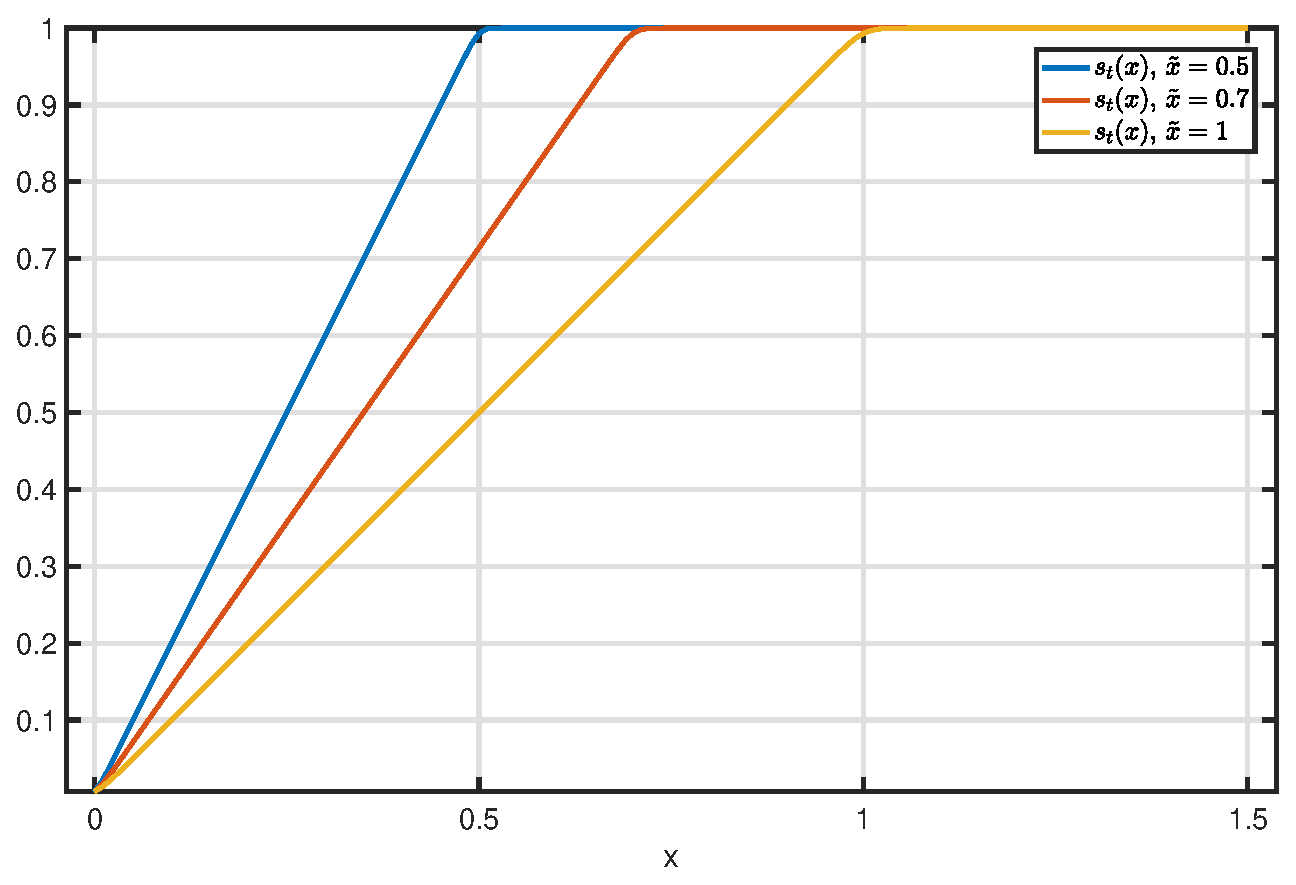
\includegraphics[width=0.5\textwidth]{images/Ch3/saturation.eps}
% figure caption is below the figure
\caption{Proposed saturation function $s_t(x)$ for $\kappa_s=100$, $\Tilde{x}=0.5$, $\Tilde{x}=0.7$ and  $\Tilde{x}=1$.}
\label{fig:st}       % Give a unique label
\end{figure}
\\
 Note that the value $\Tilde{x}$ has to be chosen in order to ensure that, when only one component is projected on the mesh element's centroid, the maximum value of projected local volume fraction  is still equal to 1:
 \begin{eqnarray}
    \label{eq:tilde}
    \Tilde{x}_a=\Tilde{x}_{KS}=\Tilde{x}_{pn}=1\\
    \Tilde{x}_{KS}^l= 1+\frac{1}{\kappa}\log{\left(\frac{1+(n-1)e^{-\kappa}}{n}\right)}\\
    \Tilde{x}_{pm}= \left(\frac{\left(n-1\right)z_p^\kappa+\left(z_p+1\right)^{\kappa}}{n}\right)^{\frac{1}{\kappa}}-z_p\\
    \Tilde{x}_{IE}=\frac{1}{1+(n-1)e^{-\kappa}}
    \label{eq:tilde_end}
 \end{eqnarray}
 The results of the application of the saturation function is applied to the smooth approximation of the maximum operator and is illustrated in figures \ref{fig:pbs},\ref{fig:kbs},\ref{fig:ibs} .
 \begin{figure}[!ht]
 \centering
% Use the relevant command to insert your figure file.
% For example, with the graphicx package use
  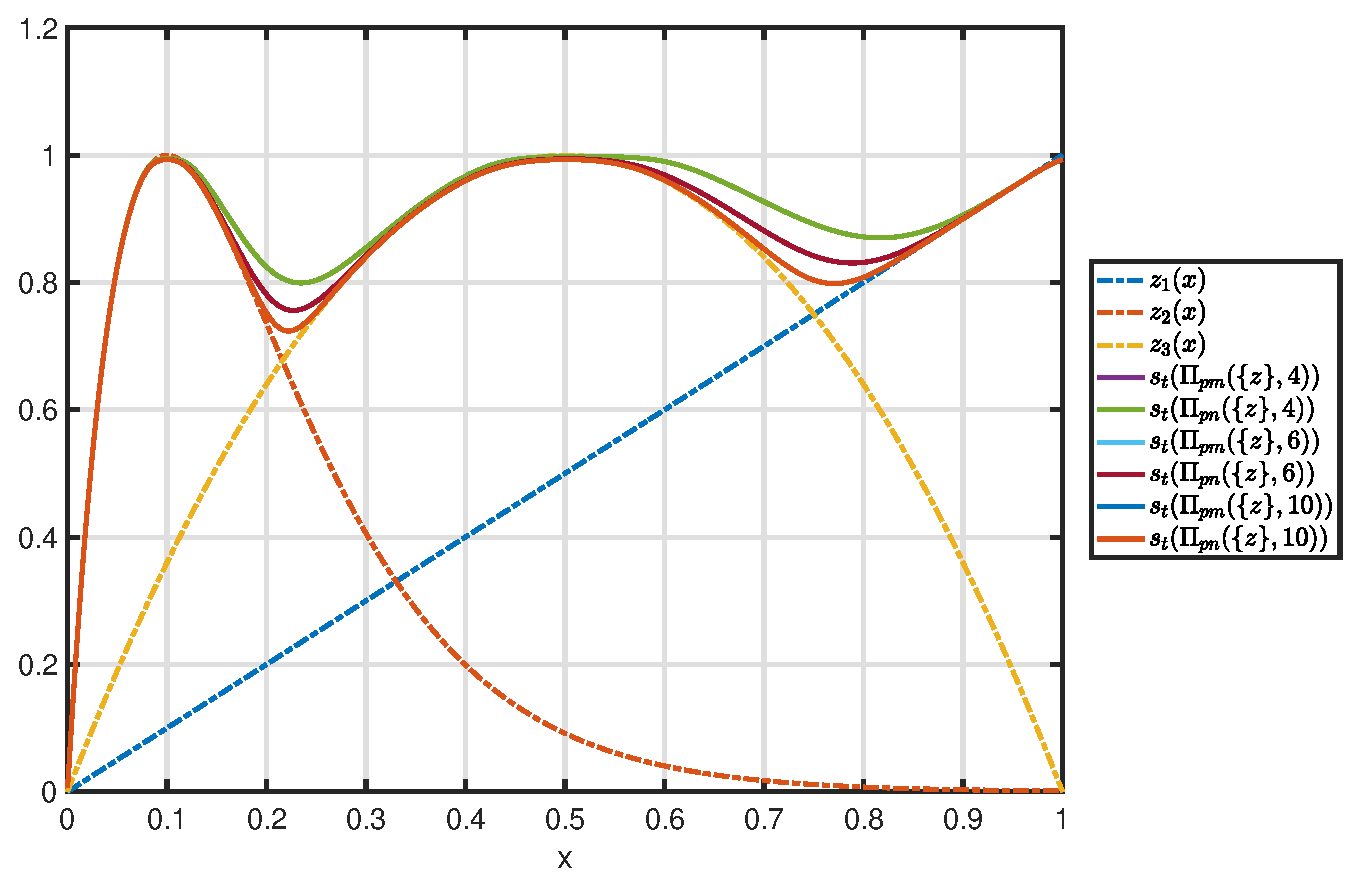
\includegraphics[width=0.5\textwidth]{images/Ch3/pmpnbenchsat.eps}
% figure caption is below the figure
\caption{Application of the proposed saturated p-norm $s_t(\Pi_{pn})$ and p-mean $s_t(\Pi_{pm})$ operator for $\kappa=4,6,10$ to the vector $\mathbf{z}$ of 3 variables,$z_1(x)=x,z_2(x)=10xe^{1-10x},z_3(x)=4x(1-x)$. One can observe the effect of the saturation since, there are no saturated value greater than 1. Moreover for $x=1$ and $x=0$, when just one component of the vector  $\vecvar{z}$ are equal to 1 and the others are 0, the saturation ensures again a value of 1.}
\label{fig:pbs}       % Give a unique label
\end{figure}
 \begin{figure}[!ht]
 \centering
% Use the relevant command to insert your figure file.
% For example, with the graphicx package use
  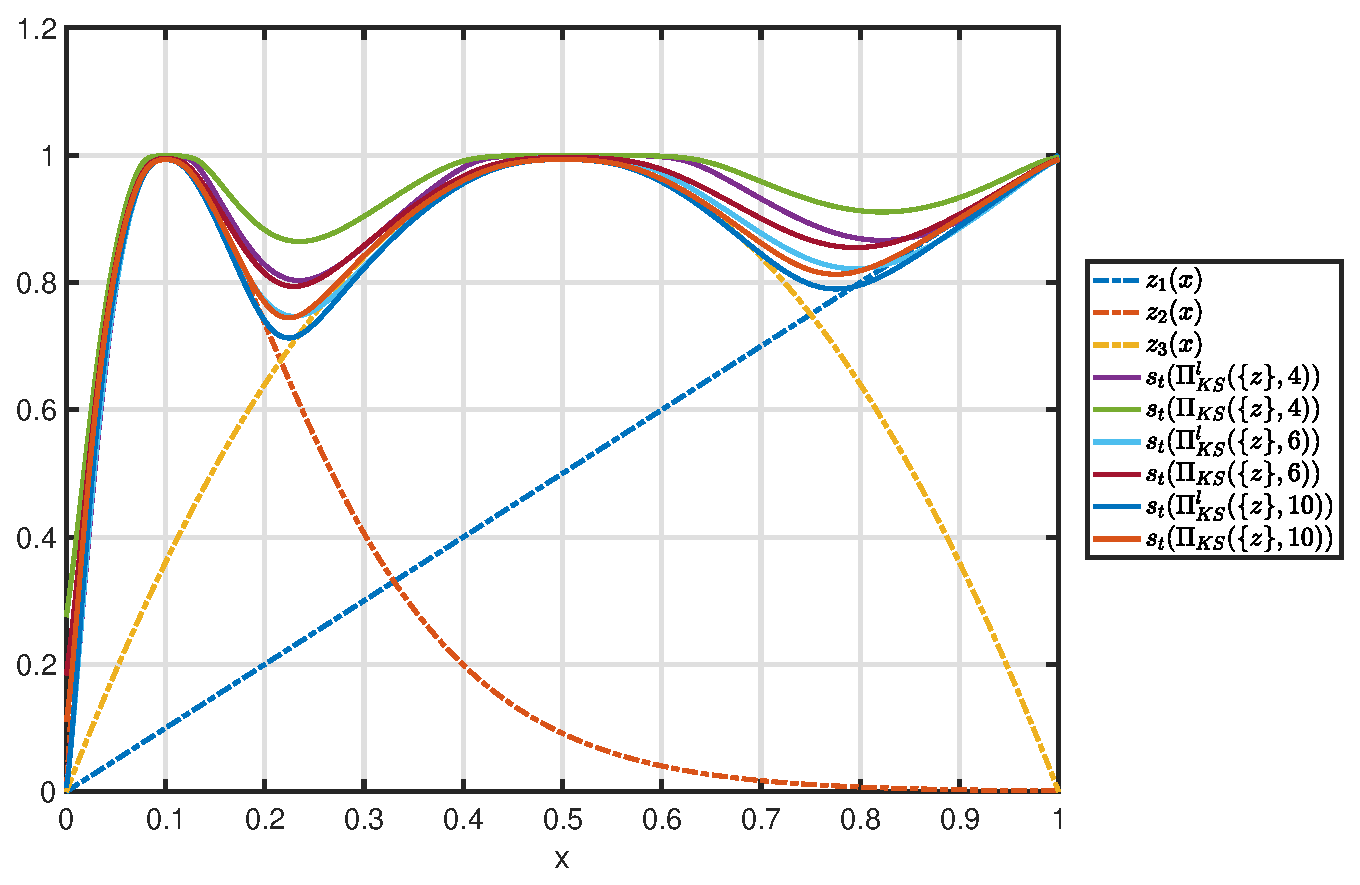
\includegraphics[width=0.5\textwidth]{images/Ch3/KSbenchsat.eps}
% figure caption is below the figure
\caption{Application of the proposed saturated KS $s_t(\Pi_{KS})$ and lower bound KS $s_t(\Pi_{KS}^l)$ function for $\kappa=4,6,10$ to the vector $\vecvar{z}$ of 3 variables, $z_1(x)=x,z_2(x)=10xe^{1-10x},z_3(x)=4x(1-x)$. One can observe the effect of the saturation since, there are no saturated value greater than 1. Moreover for $x=1$ and $x=0$, when just one component of the vector  $\vecvar{z}$ are equal to 1 and the others are 0, the saturation ensures again a value of 1. }
\label{fig:kbs}       % Give a unique label
\end{figure}
\begin{figure}[!ht]
\centering
% Use the relevant command to insert your figure file.
% For example, with the graphicx package use
  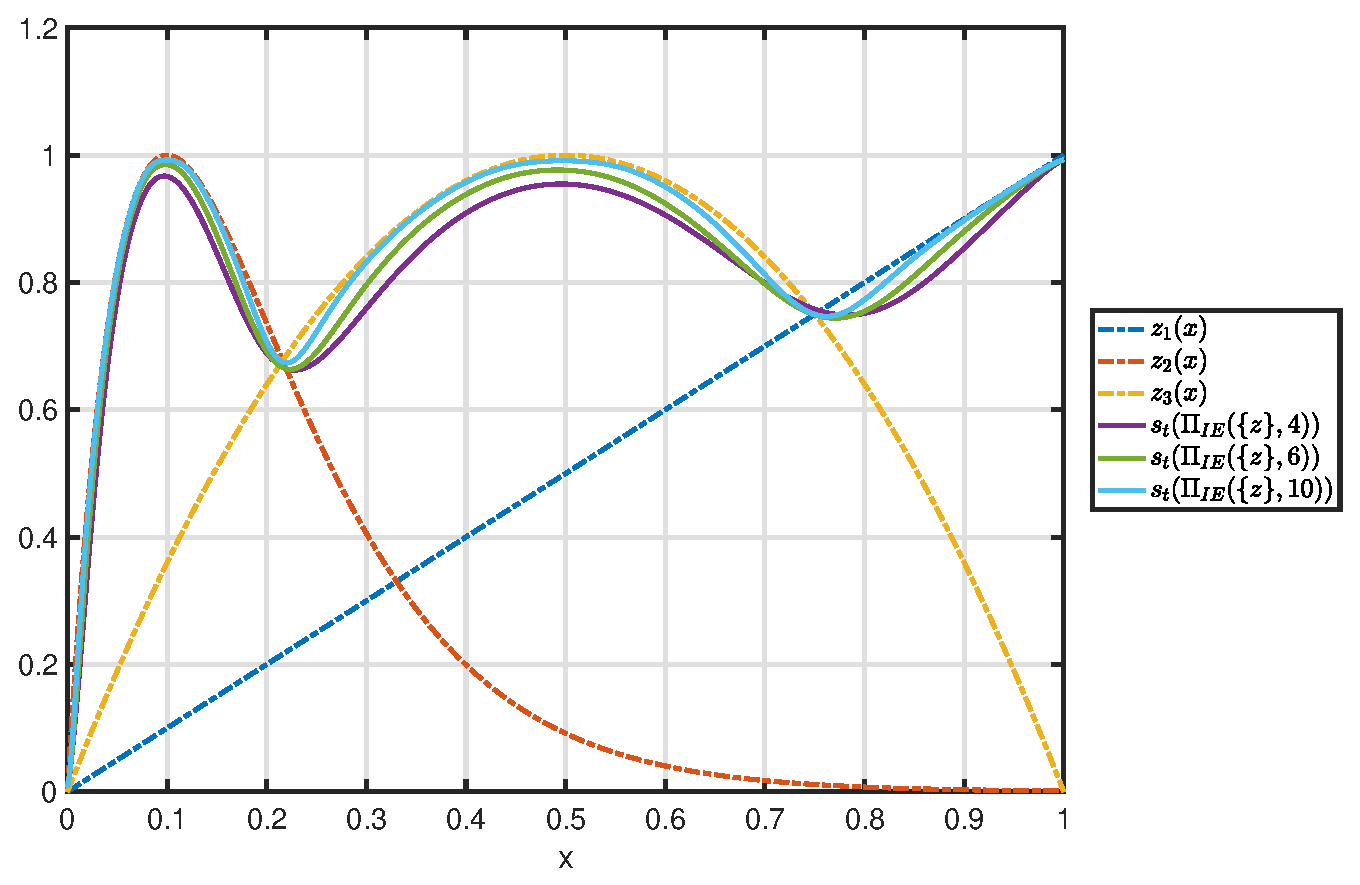
\includegraphics[width=0.5\textwidth]{images/Ch3/iebenchsat.eps}
% figure caption is below the figure
\caption{Application of the proposed saturated induced exponential aggregation function $s_t(\Pi_{IE})$ for $\kappa=4,6,10$ to the vector $\mathbf{z}$ of 3 variables,$z_1(x)=x,z_2(x)=10xe^{1-10x},z_3(x)=4x(1-x)$. One can observe the effect of the saturation since, there are no saturated values greater than 1. Moreover for $x=1$ and $x=0$, when just one component of the vector  $\vecvar{z}$ are equal to 1 and the others are 0, the saturation ensures again a value of 1.}
\label{fig:ibs}       % Give a unique label
\end{figure}
 One can observe that even when only one component projects to a local volume fraction of 1, the corresponding saturated local volume fraction is nearly at the value of 1 for all reviewed approaches. In order to show the effect of the components assembly and of the saturation, several approaches have been tested on the same configuration and the results presented in figure \ref{fig:asbly}. Another important remark is that without the saturation the p-mean, lower bound KS and induced exponential operator do not achieve the desired final density, i.e. $\rho^{el}$ is not 1 when just one of the two components projects to a density of 1. On the other hand this issue is correctly addressed by the saturation procedure proposed here. \newpage
\begin{figure*}[!ht]
\centering
 	\subfloat[asymptotic]{{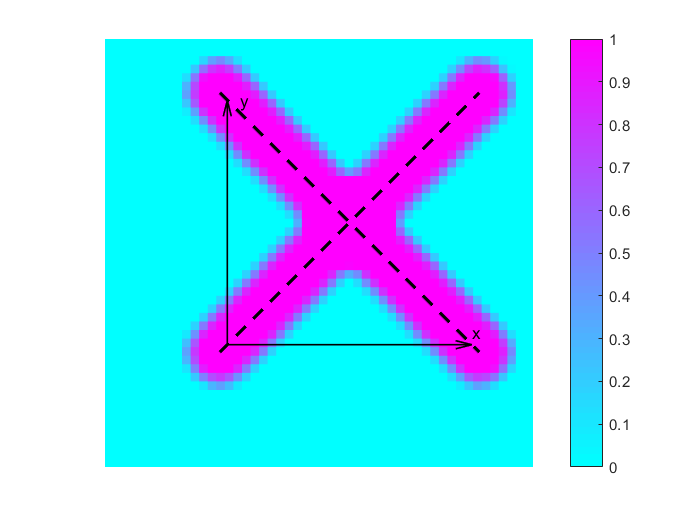
\includegraphics[width=0.35\textwidth]{images/Ch3/asymptotic.png} }}%
    \quad
    \subfloat[boolean]{{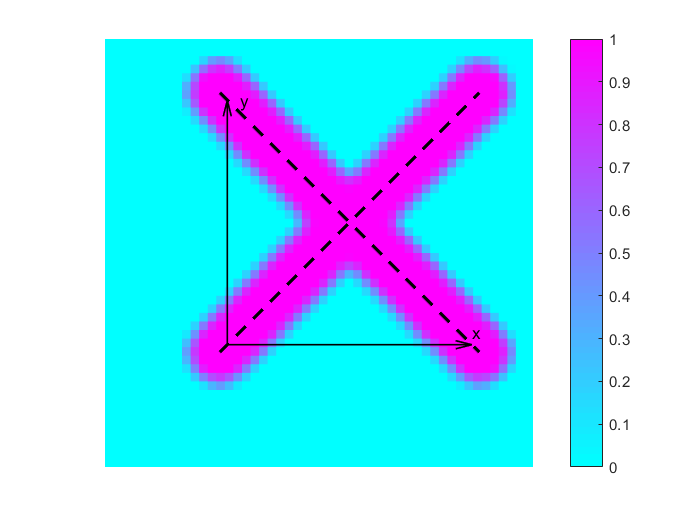
\includegraphics[width=0.35\textwidth]{images/Ch3/boolean.png} }}%
    \\
    \subfloat[p-mean, $z_p=1$]{{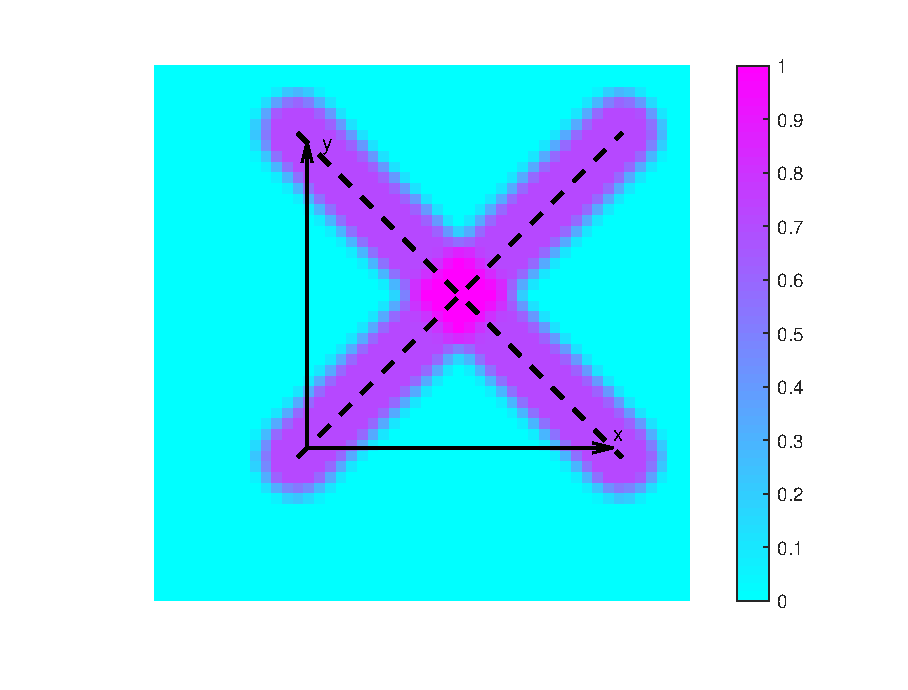
\includegraphics[width=0.35\textwidth]{images/Ch3/pmean.eps} }}%
    \quad
    \subfloat[saturated p-mean, $z_p=1$]{{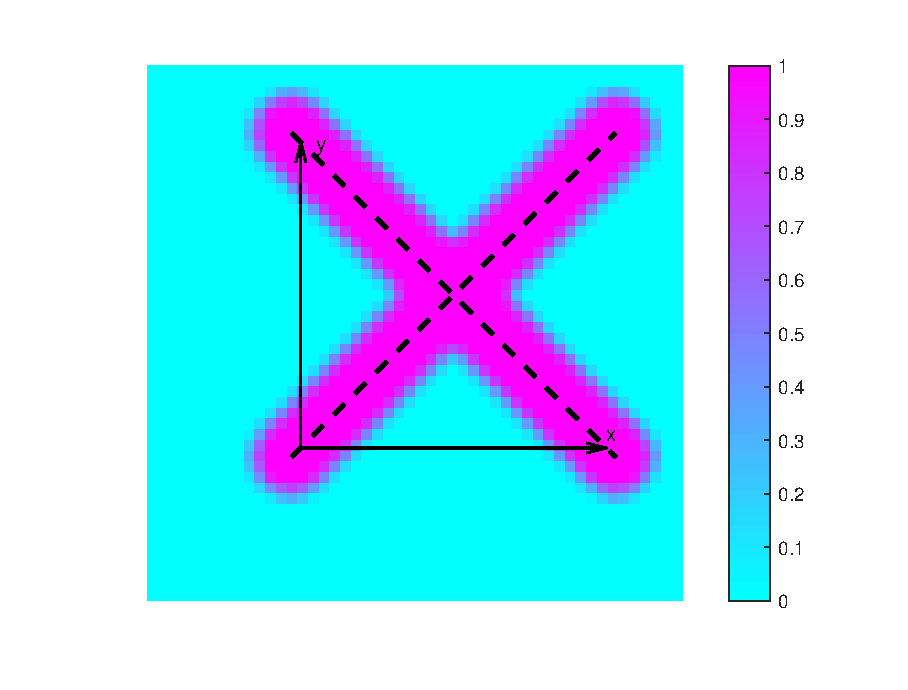
\includegraphics[width=0.35\textwidth]{images/Ch3/pmeans.eps} }}%
    \\
    \subfloat[lower bound KS]{{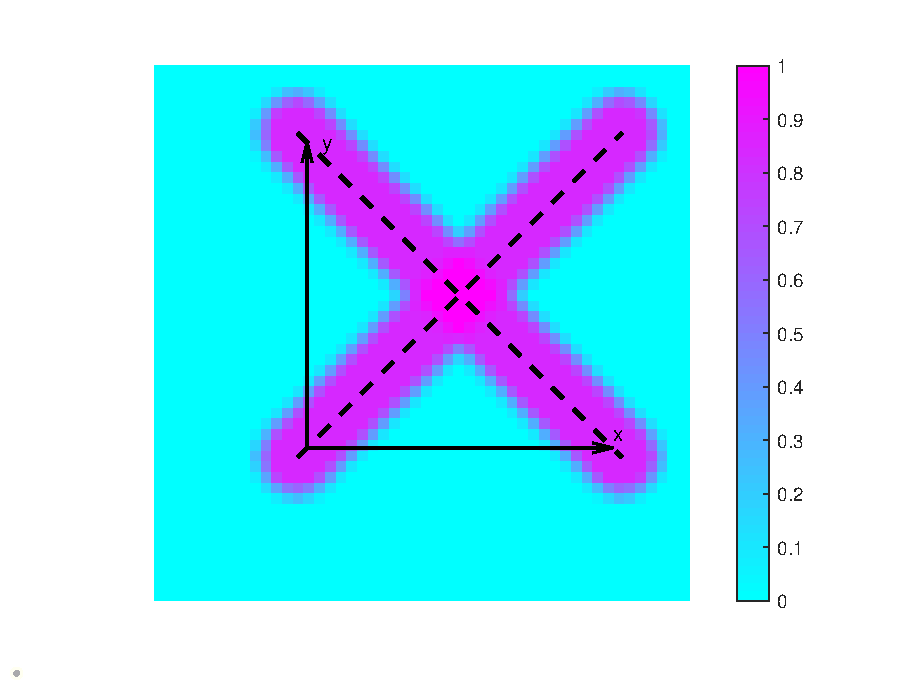
\includegraphics[width=0.35\textwidth]{images/Ch3/KSl.eps} }}%
    \quad
    \subfloat[saturated lower bound KS]{{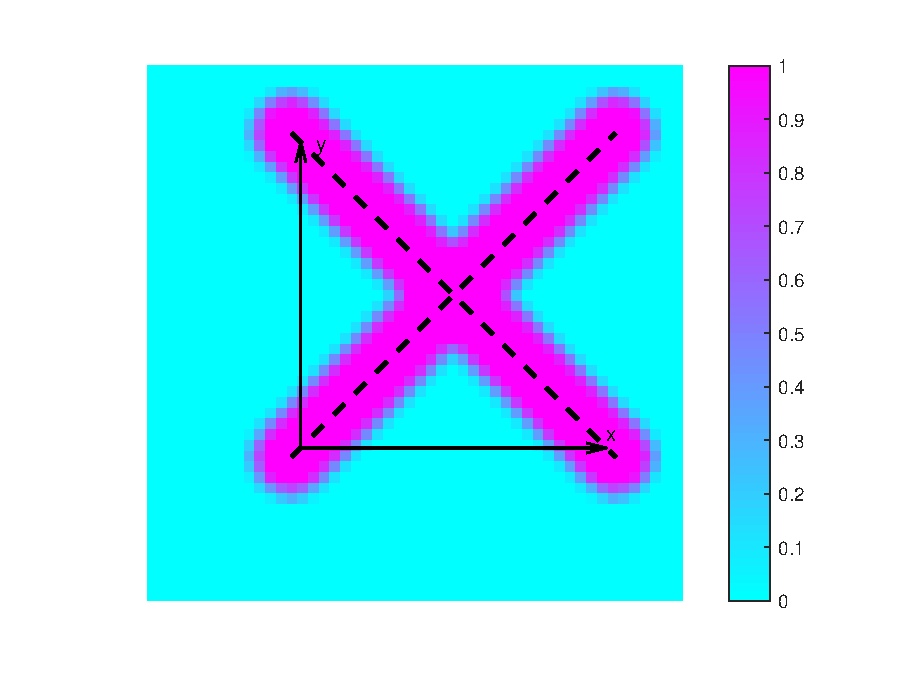
\includegraphics[width=0.35\textwidth]{images/Ch3/KSls.eps} }}%
    \\
    \subfloat[Induced exponential]{{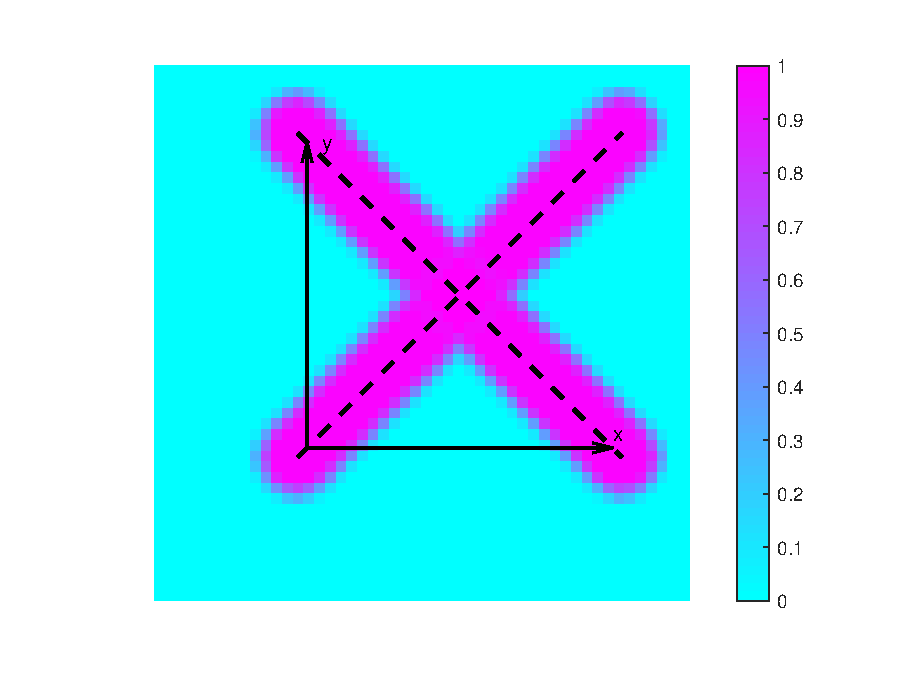
\includegraphics[width=0.35\textwidth]{images/Ch3/IE.eps} }}%
    \quad
    \subfloat[Saturated induced exponential]{{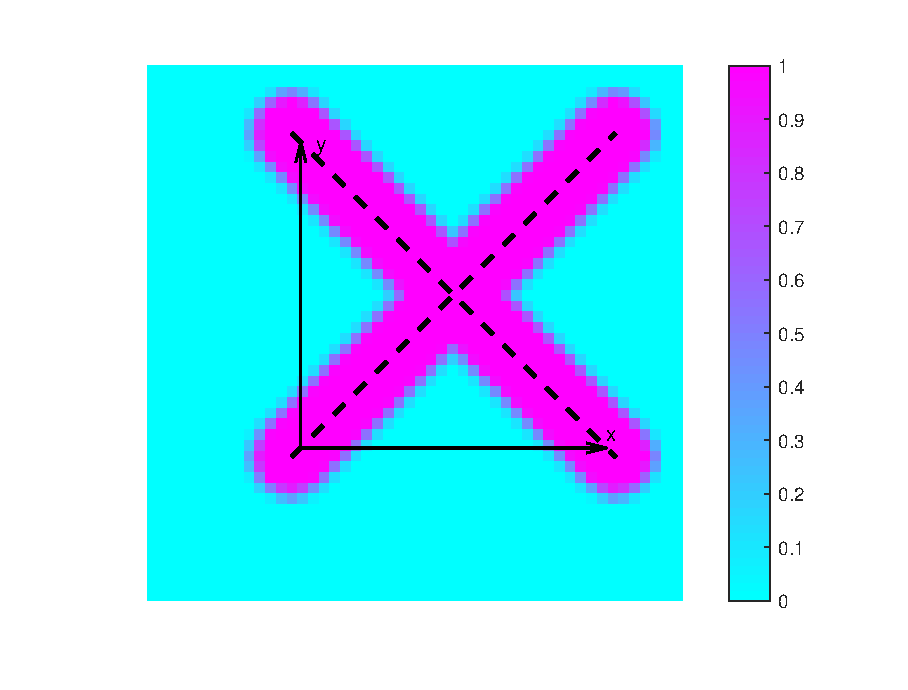
\includegraphics[width=0.35\textwidth]{images/Ch3/IEs.eps} }}%
    \caption{Distribution of $ \rho^{el}$  for two components for various assembly operators and application or not of saturation. One of the components is in the same configuration of figure \ref{fig:sc}, the other with $\theta=-\frac{\pi}{4}$ and for a $50\times50$ mesh over the domain of $X_g$. We considered AMNA with $, \gamma=3, \varepsilon=0.07, \kappa=4, \kappa_s=100$. Where $dx=0.07$ is the mesh size along the x direction.\label{fig:asbly}}%
\end{figure*}
\clearpage
\section{Sensitivity analysis}
\label{SA}
In this subsection we derive and analyze the gradient of the responses (compliance $C$ and volume fraction $V$) involved in solving the topology optimization problem considered in equation (\ref{eq:12}). The aim of this sensitivity analysis is to provide recommendations with respect to good parameter choices in the proposed Generalized Geometric Projection method. 

For compliance $C$ and volume fraction $V$ we compute by chain rule:
\begin{eqnarray}
\frac{\partial C}{\partial x_i}=\sum_{el=1}^{N_{el}}{\frac{\partial C}{\partial E^{el}}\frac{\partial E^{el}}{\partial x_i}}\\
\frac{\partial V}{\partial x_i}=\sum_{el=1}^{N_{el}}{\frac{\partial V}{\partial \rho^{el}}\frac{\partial \rho^{el}}{\partial x_i}}
\end{eqnarray}
where $N_{el}$ is the number of finite element in the mesh. This can compactly be reformulated as:
\begin{eqnarray}
\label{eq:sensC}
\left\lbrace\frac{\partial C}{\partial x}\right\rbrace=\left[\frac{\partial E}{\partial x}\right]\left\lbrace\frac{\partial C}{\partial E}\right\rbrace\\
\left\lbrace\frac{\partial V}{\partial x}\right\rbrace=\left[\frac{\partial \rho}{\partial x}\right]\left\lbrace\frac{\partial V}{\partial\rho}\right\rbrace
\label{eq:sensV}
\end{eqnarray}
In equations (\ref{eq:sensC},\ref{eq:sensV}), the right hand side vectors (of size $N_{el}\times 1$) are not different from the one computed for density based topology optimization. On the other hand the matrices $\left[\frac{\partial E}{\partial x}\right],\left[\frac{\partial \rho}{\partial x}\right]$ ( of size $N_v\times N_{el}$) are specific to the Generalized Geometry Projection method.  Let's derive their analytic expression:
\begin{equation}
    \left[\frac{\partial E}{\partial x}\right]=\left[\frac{\partial \mathbb{M}}{\partial x}\right]=\sum_{i=1}^n{\left[\frac{\partial \delta_i}{\partial x}\right]\left[\frac{\partial \mathbb{M}}{\partial \delta_i}\right]}
\end{equation}
\begin{equation}
    \left[\frac{\partial \rho}{\partial x}\right]=\left[\frac{\partial \mathbb{V}}{\partial x}\right]=\sum_{i=1}^n{\left[\frac{\partial \delta_i}{\partial x}\right]\left[\frac{\partial \mathbb{V}}{\partial \delta_i}\right]}
\end{equation}
where $\left[\frac{\partial \mathbb{M}}{\partial \delta_i}\right]$ and $\left[\frac{\partial \mathbb{V}}{\partial \delta_i}\right]$ are $N_{el}\times N_{el}$ diagonal matrices and the terms $\left[\frac{\partial \delta_i}{\partial x}\right]$ are matrices of size  $N_v\times N_{el}$. A first important observation is that $\left[\frac{\partial \delta_i}{\partial x}\right]$ is sparse and only the lines of variables belonging to the $i^{th}$ component will be different from zero i.e. $\left[\frac{\partial \delta_i}{\partial x_i}\right]$ ($6\times N_{el}$). This means that each row of $\left[\frac{\partial E}{\partial x}\right],\left[\frac{\partial \rho}{\partial x}\right]$ will have just one contribution coming from the component defined by the corresponding variable. Let's first derive the terms in the diagonal of $\left[\frac{\partial \mathbb{M}}{\partial \delta_i}\right]$ and $\left[\frac{\partial \mathbb{V}}{\partial \delta_i}\right]$. As an example here we considered MNA characteristic functions and the saturation function applied after the geometry assembly:
\begin{equation}
  \frac{\partial \mathbb{M}^{el}}{\partial \delta_i^{el}} =\frac{\partial \mathbb{M}^{el}}{\partial P_s}\frac{\partial P_s}{\partial \Pi}\frac{\partial \Pi}{\partial\delta_i^{el}}
\end{equation}
\begin{equation}
  \frac{\partial \mathbb{V}^{el}}{\partial \delta_i^{el}} =\frac{\partial \mathbb{V}^{el}}{\partial P_s}\frac{\partial P_s}{\partial \Pi}\frac{\partial \Pi}{\partial\delta_i^{el}}
\end{equation}
The evaluation of $\frac{\partial \mathbb{M}^{el}}{\partial s_t}$ and of $\frac{\partial \mathbb{V}^{el}}{\partial s_t}$ depends on the choice made among the existing functions. For AMNA one gets:
\begin{equation}
\frac{\partial \mathbb{M}^{el}}{\partial P_s}=p_b(E-E_{min})s_t^{pb-1}   
\end{equation}
\begin{equation}
\frac{\partial \mathbb{V}^{el}}{\partial P_s}=1   
\end{equation}
For the saturation function one can get:
\begin{equation}
    \frac{\partial P_s}{\partial \Pi}=\frac{\exp\left(\mathrm{\kappa_s}{\frac{\mathrm{\Pi}}{\Tilde{\Pi}}}\right)\,{\left(\exp{\left(\mathrm{\kappa_s}\frac{\mathrm{\Pi}}{\Tilde{\Pi}}\right)}+1\right)}^{-2}}{\Tilde{\Pi}\,\left(\exp{\left(-\mathrm{\kappa_s}\right)}+\frac{1}{\exp{\left(\mathrm{\kappa_s}\frac{\mathrm{\Pi}}{\Tilde{\Pi}}\right)}+1}\right)}\frac{1}{1-s_b(0,\kappa_s)}
\end{equation}
Where $\Tilde{\Pi}$ has to be computed according to equations (\ref{eq:tilde}-\ref{eq:tilde_end}).
For the computation of $\frac{\partial \Pi}{\partial\delta_i^{el}}$ the interested reader can find the computation for $KS_l$, $KS$ and induced exponential in \cite{kennedy2015improved}. For p-norm and p-mean we detail their computations as follows:
\begin{equation}
    \frac{\partial \Pi_{pm}^p}{\partial\delta_i^{el}}=\frac{1}{n}\left(\delta_i^{el}+z_p\right)^{\kappa-1}\left(\frac{1}{n}\sum_{j=1}^n{\left(\delta_j^{el}+z_p\right)^{\kappa}}\right)^{\frac{1}{\kappa}-1}
\end{equation}
\begin{equation}
    \frac{\partial \Pi_{pn}^p}{\partial\delta_i^{el}}=\left(\delta_i^{el}+z_p\right)^{\kappa-1}\left(\sum_{j=1}^n{\left(\delta_j^{el}+z_p\right)^{\kappa}}\right)^{\frac{1}{\kappa}-1}
\end{equation}
For the term $\left[\frac{\partial \delta_i}{\partial x_i}\right]$ when using Gauss quadrature one has:
\begin{equation}
    \left[\frac{\partial \delta_i}{\partial x_i}\right]   = \frac{\sum_{k=1}^{N_{GP}}{\psi_k\left[\frac{\partial W_{ik}}{\partial x_i}\right]}}{\sum_{k=1}^{N_{GP}}\psi_k} 
\end{equation}
\begin{figure*}[!ht]
\centering
    \subfloat[$\frac{\partial W}{\partial X}$]{{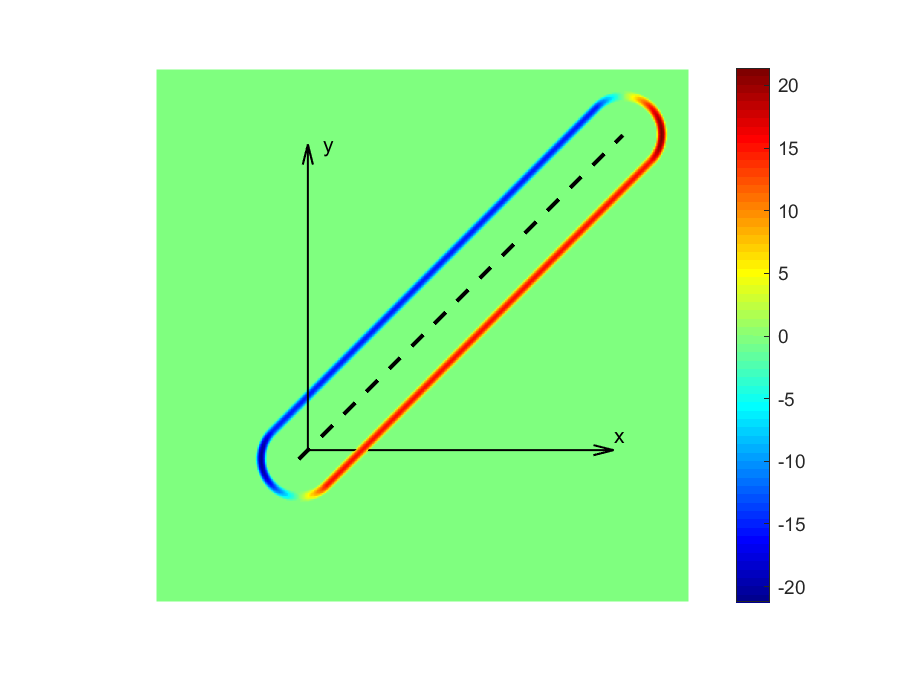
\includegraphics[width=0.35\textwidth]{images/Ch3/dW_dX.eps}}}%
    \quad
    \subfloat[$\frac{\partial \delta }{\partial X}$ ,$R=\frac{1}{2}dx$, $N_{gp}=4$]{{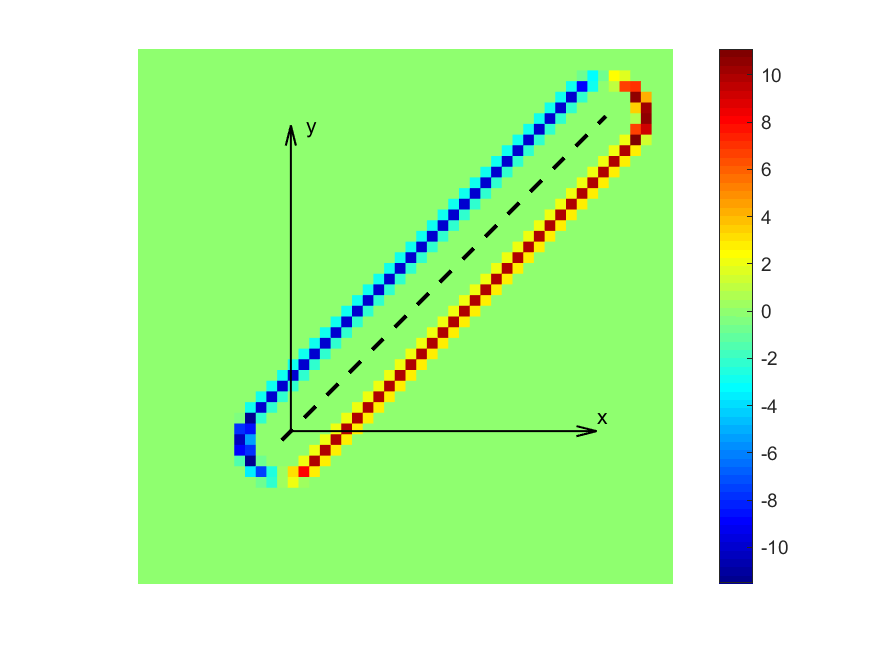
\includegraphics[width=0.35\textwidth]{images/Ch3/ddelta_dX_N_2_R_0_5.png}}}%
    \\
     \subfloat[$\frac{\partial \delta }{\partial X}$ ,$R=\frac{1}{2}dx$, $N_{gp}=9$]{{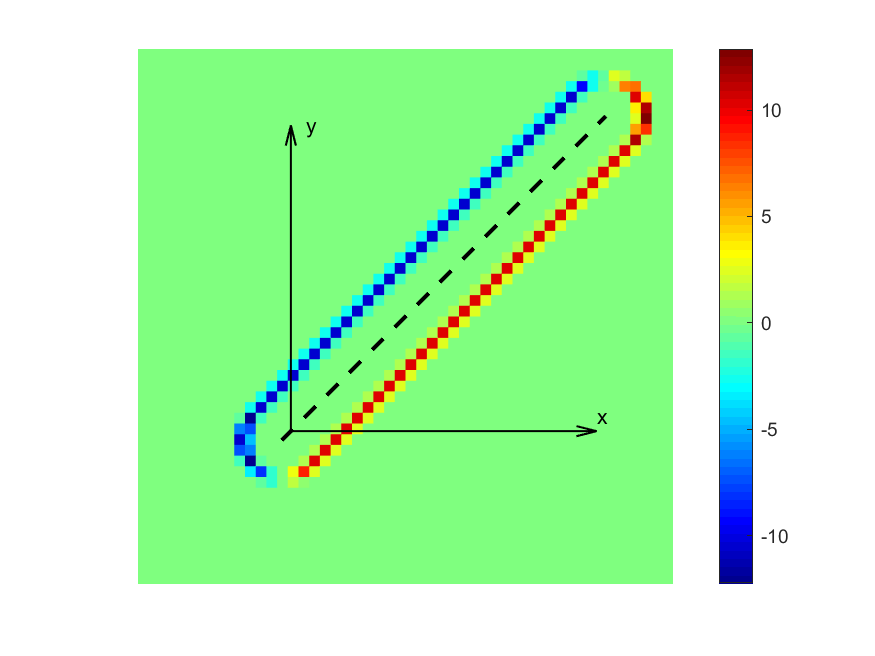
\includegraphics[width=0.35\textwidth]{images/Ch3/ddelta_dX_N_3_R_0_5.png}}}%
        \quad
        \subfloat[$\frac{\partial \delta }{\partial X}$ ,$R=dx$, $N_{gp}=4$]{{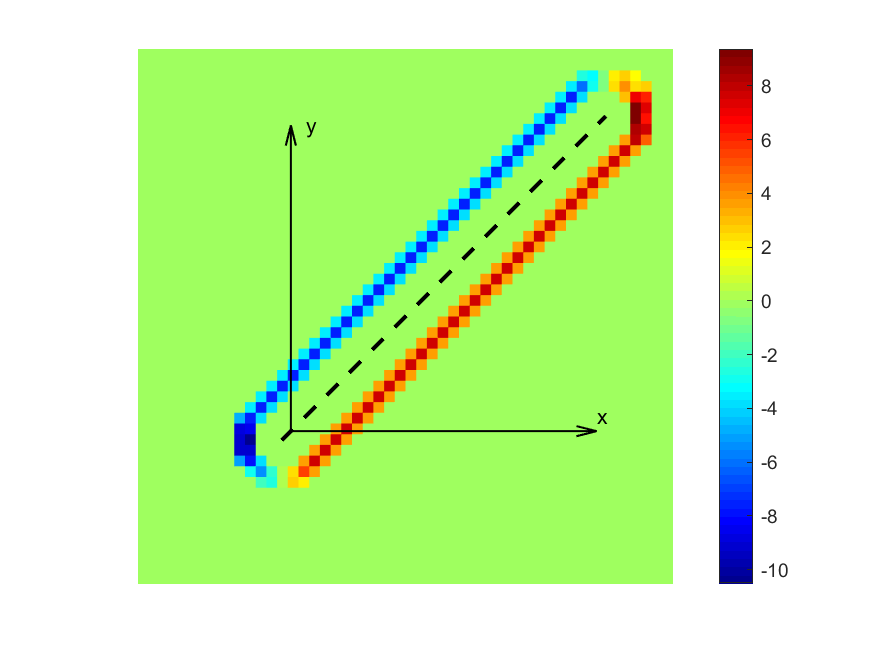
\includegraphics[width=0.35\textwidth]{images/Ch3/ddelta_dX_N_2_R_1.png}}}%
        \caption{Derivatives distribution of $W$ and $\delta$ with respect to $X$ for varying number of Gauss Points $N_{GP}$ in the sampling window and varying sampling window size $R$. We considered Adapted Moving Node Approach with the generic component of figure \ref{fig:sc} in the configuration  $X=1,Y=1,L=3,h=0.5,\theta=\frac{\pi}{4}, \gamma=3, \varepsilon=0.07$ and  $dx=0.07$ for a $50\times50$ mesh over the domain of $X_g$.}%
    \label{fig:sens_text}%
\end{figure*}
Finally for the derivatives of $\left[\frac{\partial W_{ik}}{\partial x_i}\right]$ one can again use the chain rule and the hypothesis of MNA characteristic functions. For each row of  $\left[\frac{\partial W_{ik}}{\partial x_i}\right]$  one has a different expression depending on which variable is being considered. Note that from now on, index and parenthesis notations are neglected for brevity. We can then derive the analytic expression of each derivatives, knowing that each expression has to be applied to each couple of components and point of Gauss of each sampling window. For $m$ variables one has in fact:
\begin{equation}
    \frac{\partial W}{\partial m}=\gamma m^{\gamma-1}w
\end{equation}
For variable $h$ using the chain rule:
\begin{equation}
    \frac{\partial W}{\partial h}= m^{\gamma} \vecvar{\frac{\partial w}{\partial h}}
\end{equation}
where
\begin{equation}
     \frac{\partial w}{\partial h}=\begin{cases}
         \frac{\partial a_2}{\partial h}\upsilon^2+\frac{\partial a_1}{\partial h}\upsilon+\frac{\partial a_0}{\partial h} \quad \text{if} \ l<\upsilon<u\ ,\\
         0 \quad \text{otherwise.}
    \end{cases}
\end{equation}
and where 
\begin{eqnarray}
\frac{\partial a_2}{\partial h}=-\frac{3}{\varepsilon^3}\\
\frac{\partial a_1}{\partial h}=6\frac{h}{\varepsilon^3}\\
\frac{\partial a_0}{\partial h}=3\frac{ \varepsilon^2-h^2}{4\varepsilon^3}
\end{eqnarray}
For the other components, following derivatives are obtained by the chain rule:
\begin{eqnarray}
\frac{\partial W}{\partial X}=m^\gamma\frac{\partial w}{\partial \upsilon}\left(\frac{\partial \upsilon}{\partial \varrho}\frac{\partial \varrho}{\partial X}+\frac{\partial \upsilon}{\partial \phi}\frac{\partial \phi}{\partial X}\right)\\
\frac{\partial W}{\partial Y}=m_i^\gamma\frac{\partial w}{\partial \upsilon}\left(\frac{\partial \upsilon}{\partial \varrho}\frac{\partial \varrho}{\partial Y}+\frac{\partial \upsilon}{\partial \phi}\frac{\partial \phi}{\partial Y}\right)\\
\frac{\partial W}{\partial L}=m_i^\gamma\frac{\partial w}{\partial \upsilon}\frac{\partial \upsilon}{\partial L}\\
\frac{\partial W}{\partial \theta}=m_i^\gamma\frac{\partial w}{\partial \upsilon}\frac{\partial \upsilon}{\partial \phi}\frac{\partial \phi}{\partial \theta}
\end{eqnarray}
That can be evaluated by the use of:
\begin{equation}
     \frac{\partial w}{\partial \upsilon}=\begin{cases}
         3a_3\upsilon^2+2a_2\upsilon+a_1 \quad \text{if} \ l<\upsilon<u\ ,\\
         0 \quad \text{otherwise.}
    \end{cases}
\end{equation}
\begin{equation}
   \frac{\partial \upsilon}{\partial \varrho}= \left\{ \begin{array}{ccl} \frac{2\, \varrho - L\, \left|\cos\!\left(\phi\right)\right|}{2\, \upsilon} & \text{if} & \frac{L^2}{4} < {\varrho}^2\, {\cos\!\left(\phi\right)}^2\\ \left| \sin\!\left(\phi\right)\right| & \text{if} &  \frac{L^2}{4} \geq {\varrho}^2\, {\cos\!\left(\phi\right)}^2\\ \end{array} \right.
\end{equation}
\begin{equation}
   \frac{\partial \upsilon}{\partial \phi}=\left\{\begin{array}{cl} \frac{L\,\varrho \,\mathrm{sign}\left(\cos\left(\phi \right)\right)\,\sin\left(\phi \right)}{2\,\upsilon} & \text{\ if\ \ }\frac{L^2}{4}<\varrho ^2\,{\cos\left(\phi \right)}^2\\ \varrho \,\mathrm{sign}\left(\sin\left(\phi \right)\right)\,\cos\left(\phi \right) & \text{\ if\ \ } \frac{L^2}{4}\geq\varrho ^2\,{\cos\left(\phi \right)}^2 \end{array}\right.
\end{equation}
\begin{equation}
 \frac{\partial \upsilon}{\partial L}= 
    \left\{\begin{array}{cl} \frac{\frac{L}{2}-\varrho \,\left|\cos\left(\phi \right)\right|}{2\,\upsilon} & \text{\ if\ \ }\frac{L^2}{4}<\varrho ^2\,{\cos\left(\phi \right)}^2\\ 0 & \text{\ if\ \ } \frac{L^2}{4}\geq\varrho ^2\,{\cos\left(\phi \right)}^2 \end{array}\right.
\end{equation}
\begin{eqnarray}
\frac{\partial \varrho}{\partial X}=\frac{X-x}{\varrho}\\
\frac{\partial \varrho}{\partial Y}=\frac{Y-y}{\varrho}\\
\frac{\partial \phi}{\partial X}=\frac{y-Y}{\varrho^2}\\
\frac{\partial \phi}{\partial Y}=\frac{X-x}{\varrho^2}\\
\frac{\partial \phi}{\partial \theta}=-1
\end{eqnarray}
Let us note that based on these definitions some sensitivities could be either not defined or not continuous. However note that by respecting the condition $h>\varepsilon$ these issues are avoided. In figures \ref{fig:sens_text},\ref{fig:sensY},\ref{fig:sensL},\ref{fig:sensh} and \ref{fig:sensT} the Generalized Geometry Projection is employed to study the distribution of gradients of both $W$ and $\delta$. The effect of both sampling window size and number of Gauss points is investigated. We can then make some observations and recommendations:
\begin{itemize}
    \item All represented gradient components even if defined piece-wisely are regular.
    \item All gradient components of $W$ take values different from zero only in the component's transition zone. 
    \item After applying the Generalized Geometry Projection gradient components of $\delta$ are averaged on the sampling windows and as a consequence are much smaller. Increasing the number of Gauss points, derivatives of $\delta$ become smoother, which is benefic for the optimization. Increasing the sampling window size increases the thickness of the transition zone as well as the gradients of $\delta$, which also has benefic effects as will be further illustrated in the next section.
\end{itemize}
\section{Numerical investigations on 2D use cases}
\label{I}
In this section we investigate, on several numerical applications, the effects of the various parameters (such as number of Gauss points $N_{GP}$ and sampling windows size $R$) present in the Generalized Geometry Projection, in terms of finite element analysis accuracy and topology optimization problem ill conditioning. In the first subsection we consider a simple cantilever beam that can be modelled using both the Geometry projection scheme and classic Euler beam finite element. The aims of this analysis is to investigate the model accuracy and limits when using Generalized Geometry Projection. In the topology optimization subsection we investigate the behavior of  Generalized Geometry Projection to be used for the resolution of a 2D topology optimization problem: the short cantilever beam. This problem has been widely studied by several works, here it is considered only to assess a common problem that every approach is faced with and for which we provide practical recommendations.
\subsection{Parametric study of a cantilever beam}
\label{CB}
We first consider a simple test case that can also be compared to theoretical results: the cantilever beam (c.f. figure \ref{fig:cb}).
In table \ref{tab:2} the numerical values chosen for our numerical experiment are detailed.
\begin{figure}[!h]
\centering
% Use the relevant command to insert your figure file.
% For example, with the graphicx package use
  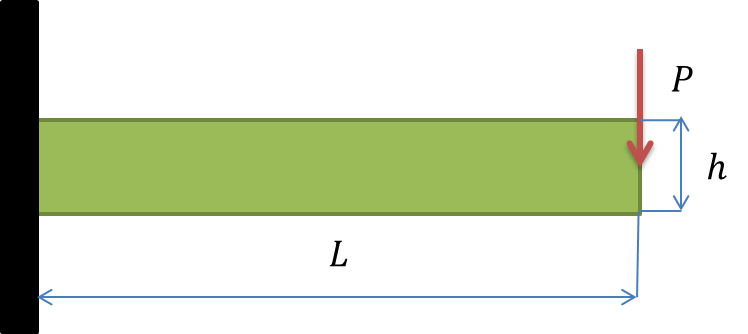
\includegraphics[width=0.5\textwidth]{images/Ch3/Cantilever_beam.png}
% figure caption is below the figure
\caption{Representation of the considered cantilever beam problem.}
\label{fig:cb}       % Give a unique label
\end{figure}
\begin{table}[h!]
% table caption is above the table
\caption{Parameters retained for the parametric study of the cantilever beam}
\label{tab:2}       % Give a unique label
\centering
% For LaTeX tables use
\begin{tabular}{lll}
\hline\noalign{\smallskip}
Parameter name & symbol & value \\
\noalign{\smallskip}\hline\noalign{\smallskip}
Material Young Modulus & $E$ & $1$\\
Beam Length & $L$ & $100$ \\
Beam width (out of plane direction) & $b$ & $1$\\
Beam height & $h$ & $\in [1,10]$ \\
Load amplitude & $P$ & $1$\\
Number of element in x direction & $n_{elx}$ & $100$\\
Number of element in y direction & $n_{ely}$ & $50$\\
Poisson ratio & $\upsilon$ & $0.3$\\
element size in x direction & $dx$ & $1$\\
element size in y direction & $dy$ & $1$\\
AMMC parameter $\alpha$ & $\alpha$ & $1$\\
AMMC parameter $\beta$ & $\beta$ & $10^{-3}$\\
AMMC parameter $\epsilon$ & $\epsilon$ & $0.7$\\
AMMC parameter $q$ & $q$ & $3$\\
AMMC parameter $\alpha$ & $\alpha$ & $1$\\
AGP parameter $r$ & $r$ & $1.5$\\
AGP/AMNA parameter $\gamma_v$ & $\gamma_v$ & $1$\\
AGP/AMNA parameter $\gamma_c$ & $\gamma_c$ & $1.5$\\
AGP parameter $\delta_{min}$ & $\delta_{min}$ & $10^{-6}$\\
AMNA parameter $\varepsilon$ & $\varepsilon$ & $3$\\
AMNA parameter $p_b$ & $p_b$ & $1$\\
AMNA parameter $E_{min}$ & $E_{min}$ & $10^{-6}$\\
Aggregation constant for saturation & $\kappa_s$ & $10^{2}$\\
\noalign{\smallskip}\hline
\end{tabular}
\end{table}
Here we will investigate the effect of thickness $h$, of the number of Gauss points $N_{GP}$ and of the sampling window size (of the Generalized Geometry Projection) $R$ as well as the effect of the topology optimization method employed (AMMC, AGP or AMNA) on the total compliance $C$ and volume fraction $V$ (defined with respect to the total volume occupied by the solid finite element mesh).
Using the well-known Euler beam model, one can in fact compute analytically the compliance and the volume fraction of the beam:
\begin{eqnarray}
C=\frac{4PL^3}{Ebh^3}=\frac{4\times 10^6}{h^3}\\
V=\frac{bLh}{n_{elx}n_{ely}}=\frac{h}{50}
\end{eqnarray}
The reader can observe that for the range of values selected for $h\in[1,10]$ the ratio between the beam length $L$ and its cross section area $A=bh$ is $\frac{L}{A}\in[10,100]$, large enough to consider the hypothesis of Euler beam model reasonable.
For this cantilever beam problem we now consider the Generalized Geometry Projection, over the mesh illustrated in figure \ref{fig:ggpcb_b}.
\begin{figure}[!ht]
\centering
    \subfloat[Component plot for the cantilever beam]{{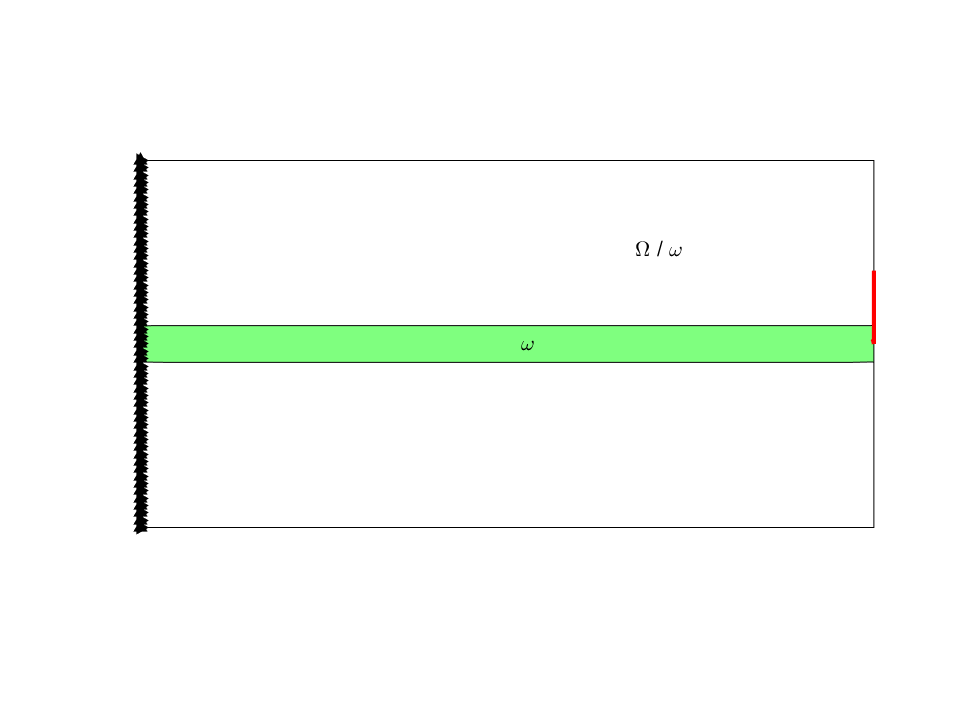
\includegraphics[width=0.5\textwidth]{images/Ch3/Cantilever_component.eps}}}%
    \subfloat[Corresponding density plot distribution $\rho^{el}$ \label{fig:ggpcb_b}]{{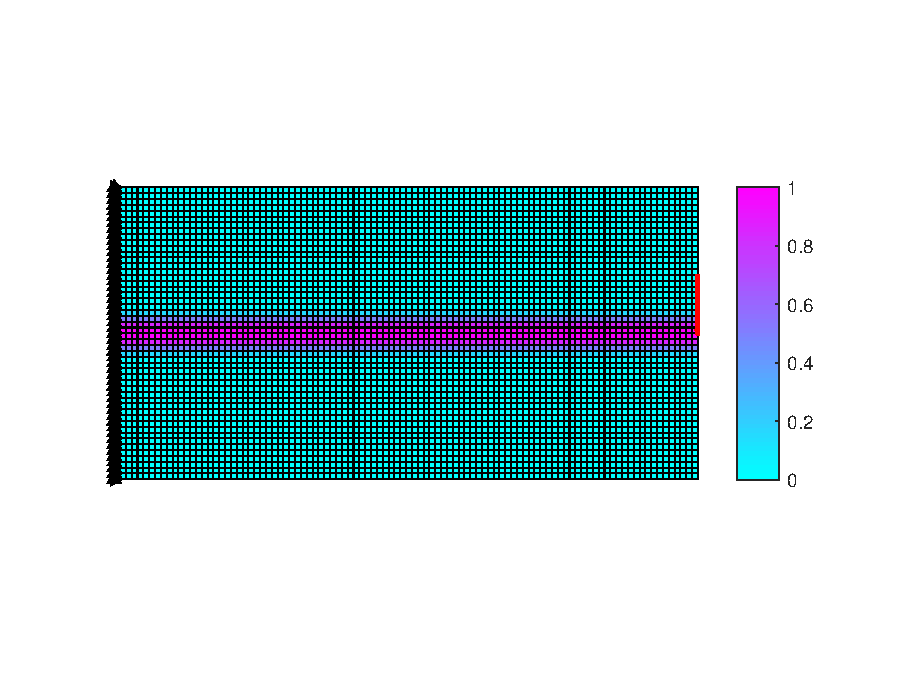
\includegraphics[width=0.5\textwidth]{images/Ch3/Cantilever_densityeps.eps}}}%
    \caption{Illustration of the Adapted Moving Node Approach (AMNA)  for the cantilever beam. A single round ended component $\omega$ is considered in the configuration $\vecvar{x}=\vecvar{50,25,100,5,0}$. The $100\times 50$ 2D planar stress solid element mesh covers the domain $\Omega\cong  [0,100] \times [0,50]$. We set $N_{GP}=1$ and $R=\frac{1}{2}dx$. The saturation function was employed. The other hyper-parameters are summarized in table \ref{tab:2}. The round ends of the components fall outside$\Omega$ and are not represented in these figures. }%
    \label{fig:ggpcb}%
\end{figure}
\begin{figure}[!ht]
\centering
    \subfloat[$h-C$ plot for $R=0.5$, $N_{GP}=\vecvar{1,4,16,64}$]{{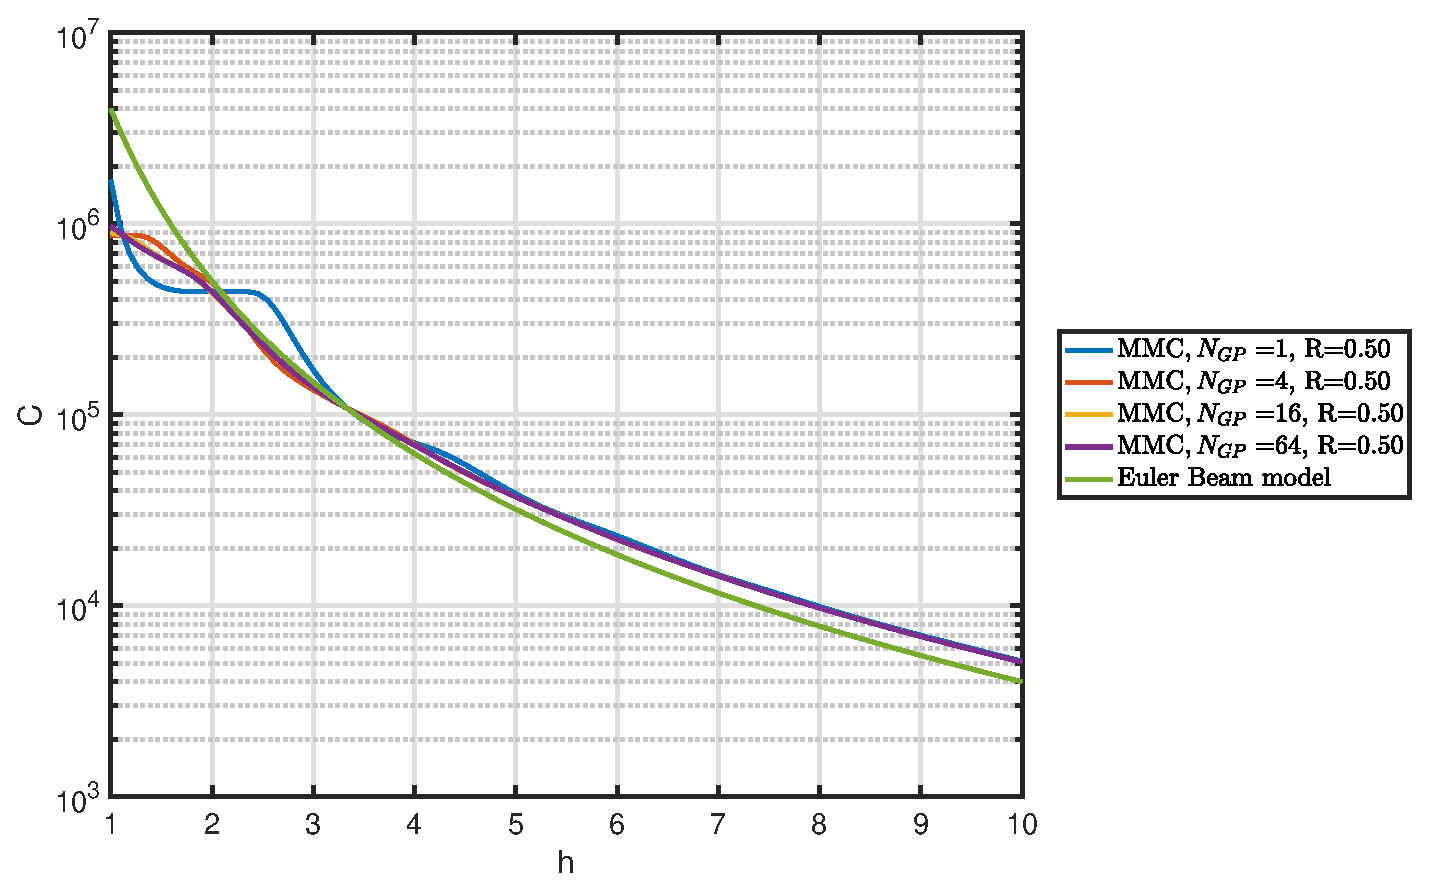
\includegraphics[width=0.5\textwidth]{images/Ch3/fig22a.eps} }}%
    \subfloat[$h-V$ plot for $R=0.5$, $N_{GP}=\vecvar{1,4,16,64}$]{{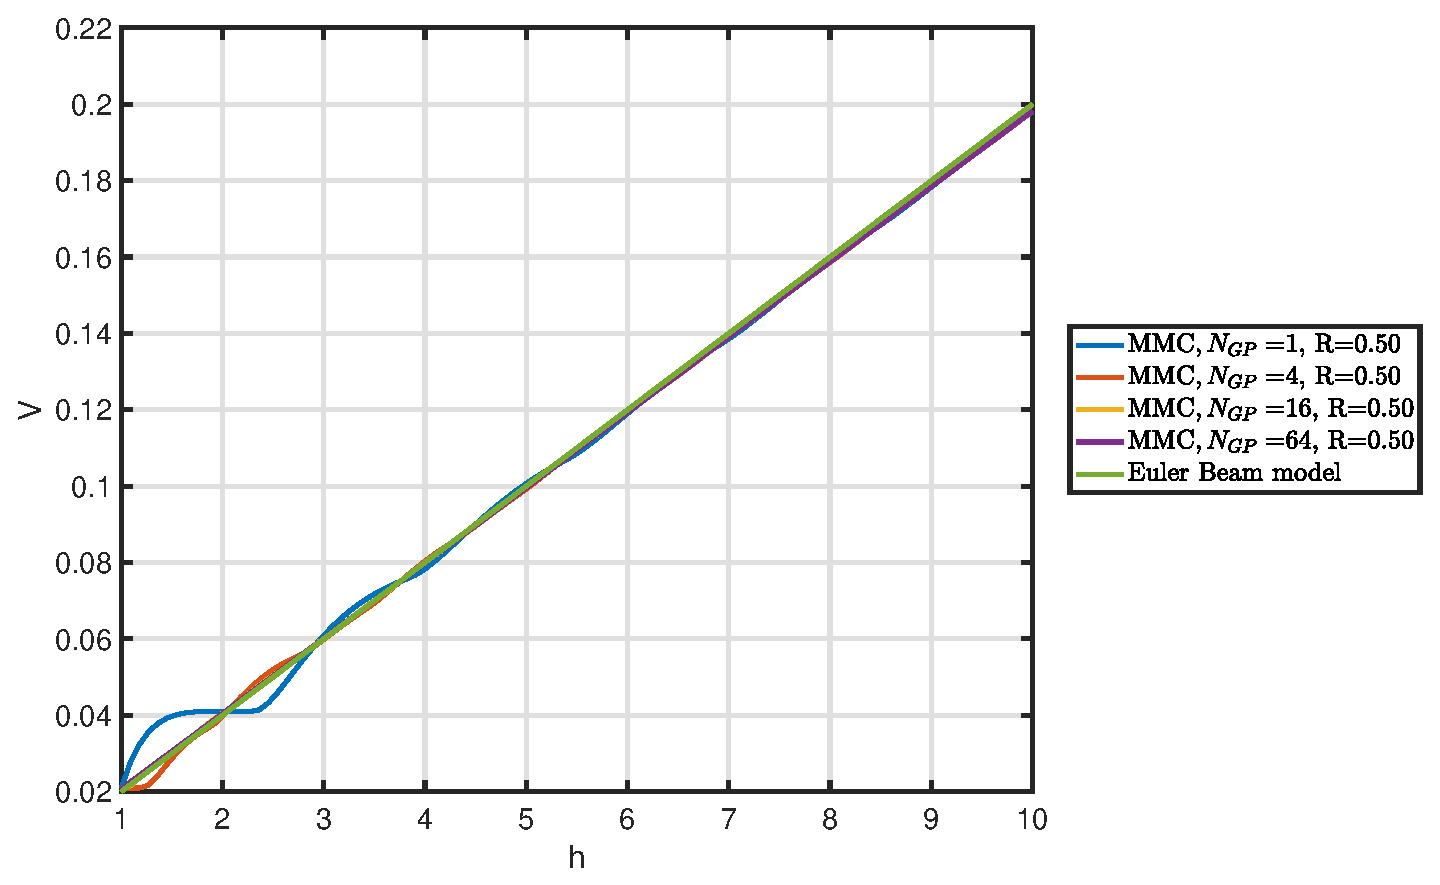
\includegraphics[width=0.5\textwidth]{images/Ch3/fig22b.eps} }}%
    \caption{Cantilever beam parametric study using the AMMC approach for $R=0.5$ . Effect of the sampling window number of Gauss points $N_{GP}$ on the structural compliance and the volume fraction. In each graph we reported in green the true theoretical values based on the analytic beam model. The remainder of results can be found in annexes.}%
    \label{fig:cbMMCtext}%
\end{figure}
The results of this trade study, which varied parameters $h$ , $N_{GP}$, $R$ and the chosen method, are shown in figures \ref{fig:cbMMCtext} and appendix figures \ref{fig:cbMMC},\ref{fig:cbGP} and \ref{fig:cbMNA}. We can make following observations:
\begin{itemize}
\item For all methods one gets better accuracy for higher thicknesses, especially for the compliance $C$. These effects are closely related to a very well-known issue of solid elements with complete integration: the shear-locking effect. The stiffness of thin structures are overestimated when using few element in the thickness direction. As a consequence the mesh size can control the minimal dimension of the components that one can consider in topology optimization without losing model accuracy.
\item For all reviewed adapted methods, mesh induced inflection points in both compliance and volume fraction graph may be observed (i.e. waviness in the respective curves). This is especially the case for small values of $h$ and of $N_{GP}$ and for AMMC. 
\item Increasing the sampling window size $R$ (for $N_{GP}>1$) reduces the model compliance.
\item Increasing the number of Gauss points $N_{GP}$, mesh induced phenomena are attenuated for all approaches. 
\end{itemize}
The model behavior is dictated by the transition region at the border of the components, especially for small $h$, which also explains why AMMC amplifies the mesh induced phenomena. In fact, the transition region thickness being proportional to $h$, for small value of $h$ and $N_{GP}$, the transition region is small enough to be located between Gauss point locations. In this situation for small changes of the thickness $h$ both $C$ and $V$ will not change, as can be seen in figure \ref{fig:cbMMC}
These observation are of course relative to our particular choice of settings for each approach and are not necessarily  generalizable to other geometric configurations. Nevertheless, based on the causes mentioned for these effects, they are likely to reoccur in many other situations. As shown, a good choice of the topology optimization parameters  $h$ , $N_{GP}$, $R$ and formulation can however reduce these negative effects.
 Finally we want to point out the fact that these conclusions are consistent with the observation made in the work of Zhou et al. \cite{zhou2016feature} for geometric feature based topology optimization using level set topology optimization.
\subsection{Topology Optimization of the short cantilever beam}
\label{SCB}
In this subsection we consider the topology optimization of a short cantilever beam, starting from an initial components configuration shown in figure \ref{fig:scb}. We will  investigate on this test case the effects of the number of Gauss points in each sampling window $N_{GP}$ on the optimization convergence, when using the adapted methods based on the proposed GGP framework: AMMC, AGP and AMNA.
 \begin{figure}[!ht]
 \centering
% Use the relevant command to insert your figure file.
% For example, with the graphicx package use
  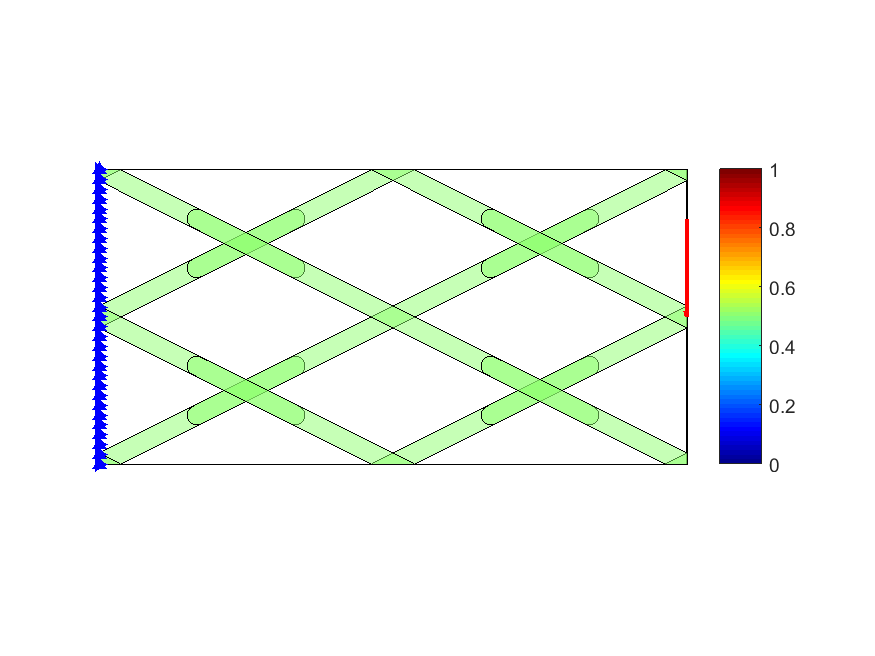
\includegraphics[width=0.5\textwidth]{images/Ch3/component_000.png}
% figure caption is below the figure
\caption{Initial configuration for the short cantilever topology optimization problem. Components are colored according to the value of $m$. Blue triangles represents clamped degrees of freedoms. The red arrow represents the applied load. 18 round ended bars are considered for the optimization, i.e. $6\times 18=108$ design variables for both AGP and AMNA and $5\times 18=90$ design variables for AMMC.}
\label{fig:scb}       % Give a unique label
\end{figure}
We employed the well know Method of Moving Asymptotes \cite{svanberg1987method}, in the Matlab version distributed by the author \cite{svanberg2004some}. A special rescaling was also adopted to avoid MMA numerical instabilities as explained in appendix \ref{A1}. A saturated KSl aggregation operator was employed to make the geometric union of component for all adapted methods.
The design variables are initiated according to figure \ref{fig:scb}. The stopping criteria employed was on the infinite norm of the configuration variation. The numerical values chosen for all the parameters of both projection and optimization solver are detailed in table \ref{tab:3}. 
\begin{table*}[h!]
% table caption is above the table
\caption{Parameters used for the parametric study of the short cantilever beam}
\label{tab:3}       % Give a unique label
\centering
% For LaTeX tables use
\begin{tabular}{lll}
\hline\noalign{\smallskip}
Parameter name & symbol & value \\
\noalign{\smallskip}\hline\noalign{\smallskip}
Material Young Modulus & $E$ & $1$\\
Design zone width (out of plane direction) & $b$ & $1$\\
Load amplitude & $P$ & $1$\\
Number of element in x direction & $n_{elx}$ & $60$\\
Number of element in y direction & $n_{ely}$ & $30$\\
Poisson ratio & $\upsilon$ & $0.3$\\
element size in x direction & $dx$ & $1$\\
element size in y direction & $dy$ & $1$\\
AMMC parameter $\alpha$ & $\alpha$ & $1$\\
AMMC parameter $\beta$ & $\beta$ & $10^{-3}$\\
AMMC parameter $\epsilon$ & $\epsilon$ & $0.866$\\
AMMC parameter $q$ & $q$ & $2$\\
AMMC parameter $\alpha$ & $\alpha$ & $1$\\
AGP parameter $r$ & $r$ & $0.5$\\
AGP/AMNA parameter $\gamma_v$ & $\gamma_v$ & $1$\\
AGP/AMNA parameter $\gamma_c$ & $\gamma_c$ & $3$\\
AGP parameter $\delta_{min}$ & $\delta_{min}$ & $10^{-6}$\\
AMNA parameter $\varepsilon$ & $\varepsilon$ & $1$\\
AMNA parameter $p_b$ & $p_b$ & $3$\\
AMNA parameter $E_{min}$ & $E_{min}$ & $10^{-6}$\\
Aggregation constant for saturation & $\kappa_s$ & $10^{2}$\\
Aggregation constant  & $\kappa$ & $10$\\
MMA moving limit & & 0.1\\
MMA initial moving limit & & 0.01\\
MMA incremental factor asyincr  & & 1.2\\
MMA decremental factor asydecr & & 0.4\\
MMA parameter albefa & & 0.1\\
MMA parameter move & & 0.5\\
Stopping criterion, design variable variation & & 0.001\\
Minimal x position & $x_{min}$ & -1\\
Minimal y position & $y_{min}$ & -1\\
Minimal length& $L_{min}$ & 0\\
Minimal height & $h_{min}$ & 1\\
Minimal angle & $\theta_{min}$ & $-2\pi$\\
Minimal component density & $m_{min}$ & 0\\
Maximal x position & $x_{max}$ & $n_{elx}+1$\\
Maximal y position & $y_{max}$ & $n_{ely}+1$\\
Maximal length& $L_{max}$ & $\sqrt{n_{elx}^2+n_{ely}^2}$\\
Maximal height & $h_{max}$ & $\sqrt{n_{elx}^2+n_{ely}^2}$\\
Maximal angle & $\theta_{max}$ & $2\pi$\\
Maximal component density & $m_{max}$ & 1\\
\noalign{\smallskip}\hline
\end{tabular}
\end{table*}
 In figure \ref{fig:scbMMC},\ref{fig:scbGP} and \ref{fig:scbMNA} the results of the topology optimization problem of a short cantilever beam are considered for several value of $N_{GP}$.
\clearpage
\begin{figure*}
\centering
\subfloat[Component plot $N_{GP}=1$, $R=\frac{1}{2}$]{{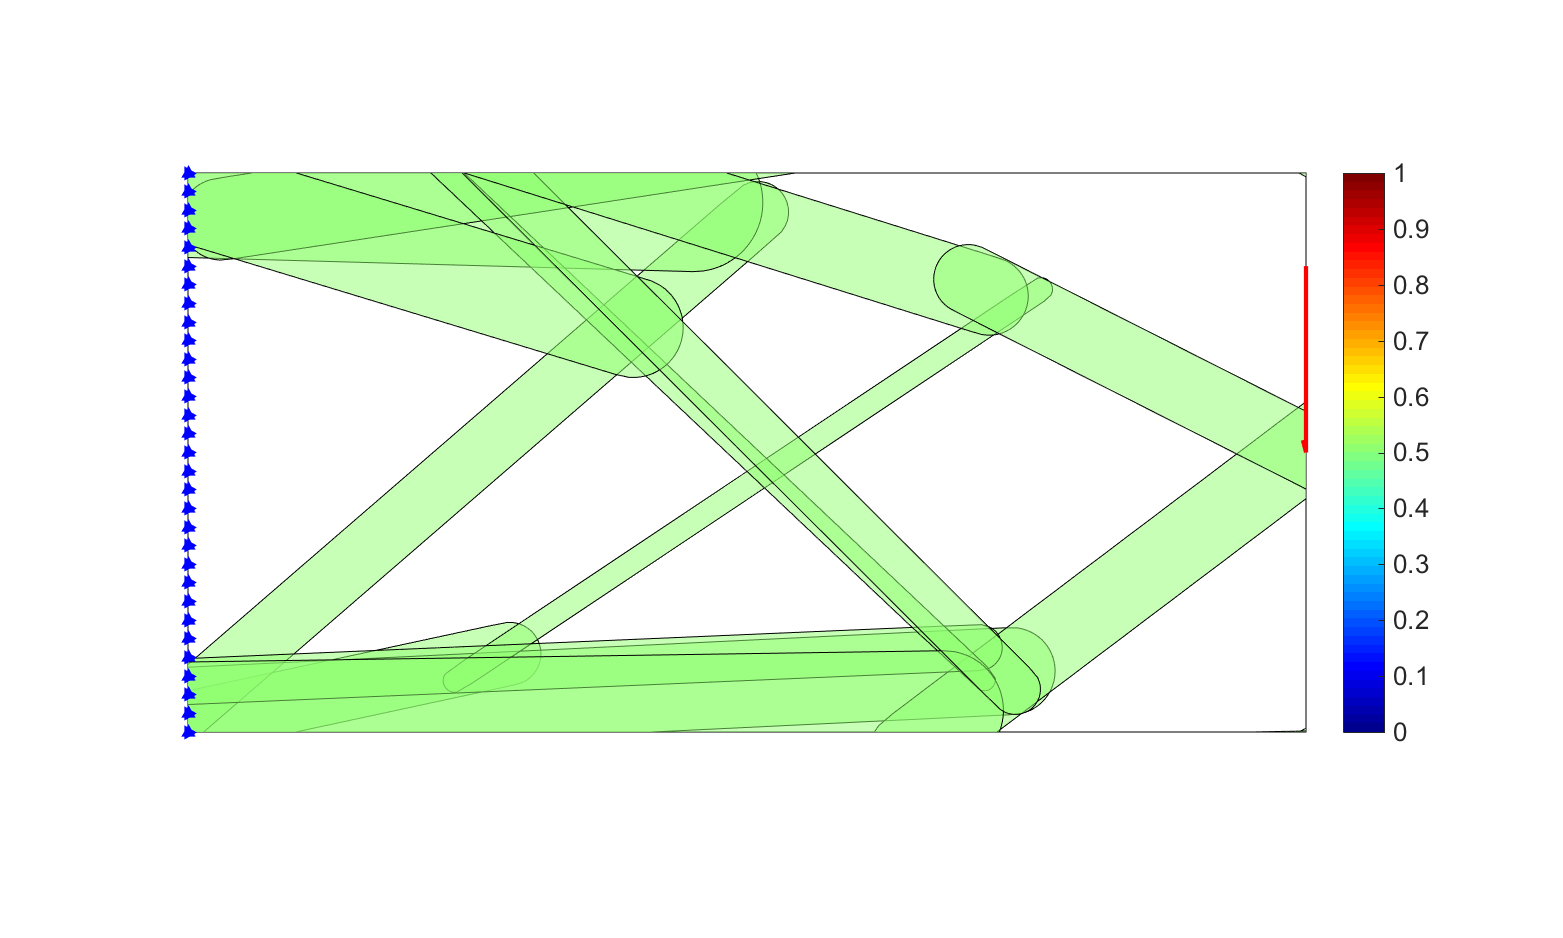
\includegraphics[width=0.3\textwidth]{images/Ch3/24a.png} }}%
\quad
\subfloat[Density plot $N_{GP}=1$, $R=\frac{1}{2}$]{{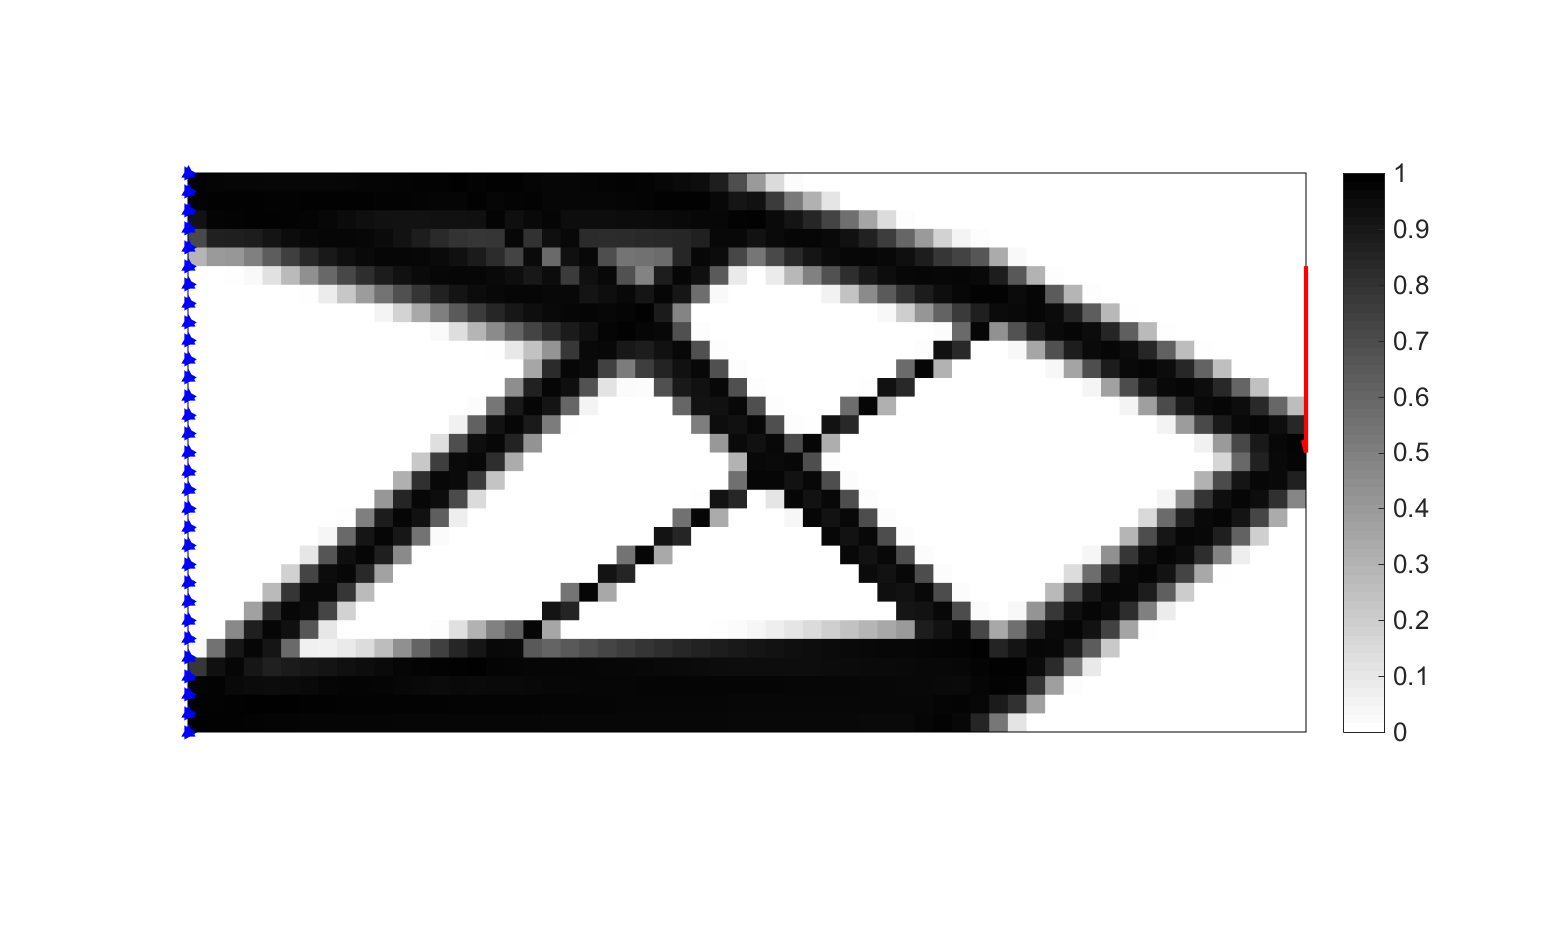
\includegraphics[width=0.3\textwidth]{images/Ch3/24b.png} }}%
    \quad
    \subfloat[Convergence plot $N_{GP}=1$, $R=\frac{1}{2}$]{{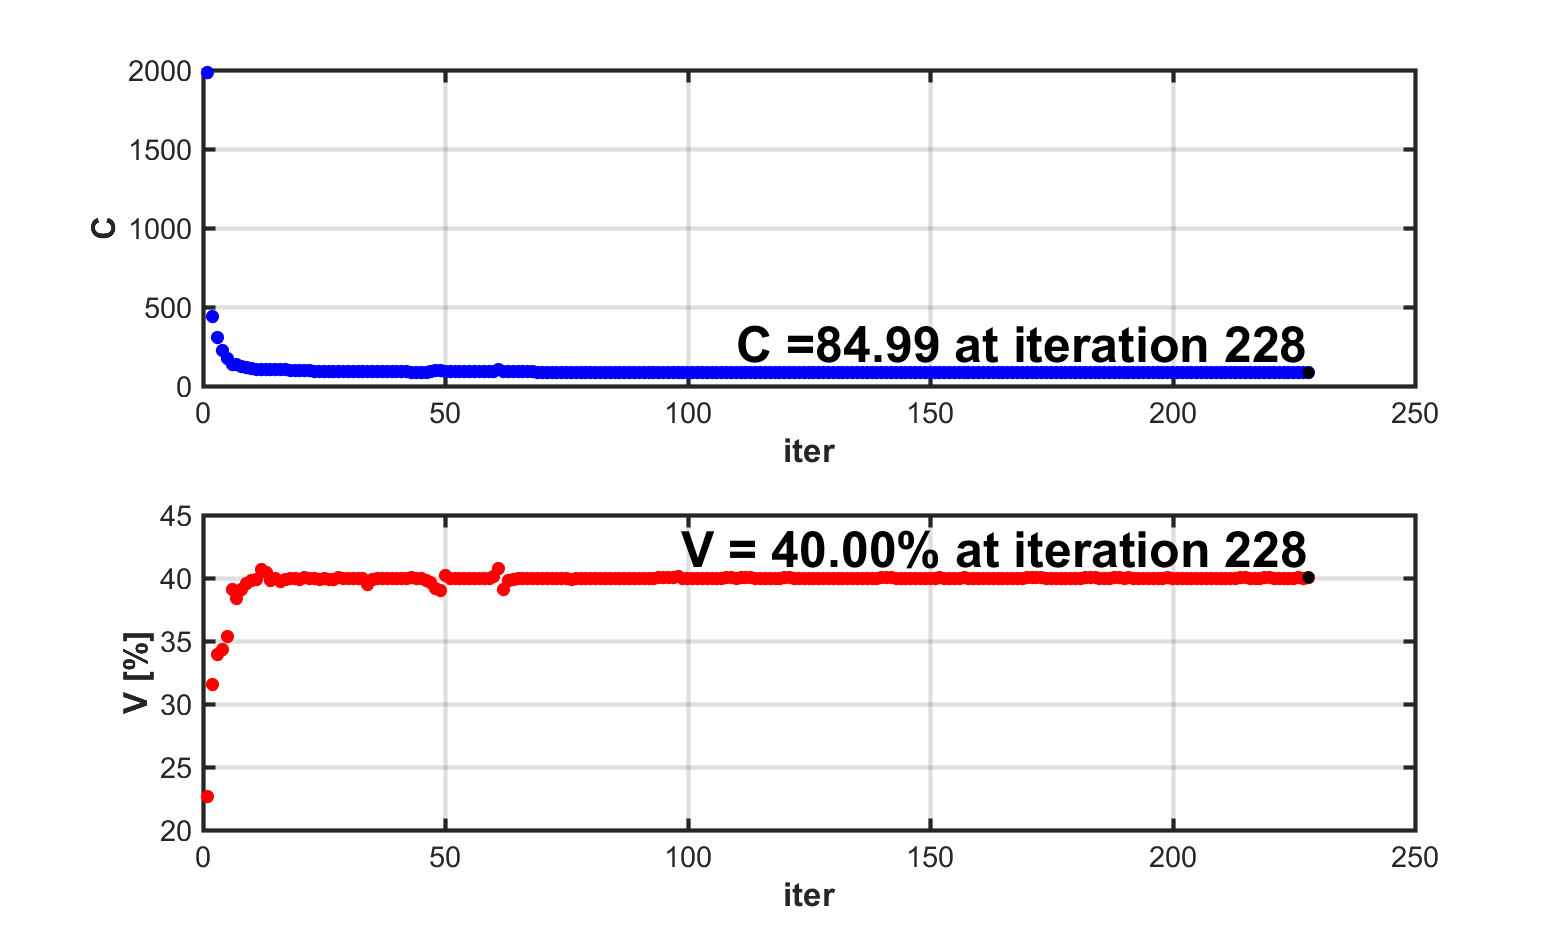
\includegraphics[width=0.3\textwidth]{images/Ch3/24c.png} }}%
        \\
\subfloat[Component plot $N_{GP}=4$, $R=\frac{1}{2}$]{{\includegraphics[width=0.3\textwidth]{images/Ch3/24d.png} }}%
\quad
 \subfloat[Density plot $N_{GP}=4$, $R=\frac{1}{2}$]{{\includegraphics[width=0.3\textwidth]{images/Ch3/24e.png} }}%
   \quad
\subfloat[Convergence plot $N_{GP}=4$, $R=\frac{1}{2}$]{{\includegraphics[width=0.3\textwidth]{images/Ch3/24f.png} }}%
 \\
 \subfloat[Component plot $N_{GP}=16$, $R=\frac{1}{2}$]{{\includegraphics[width=0.3\textwidth]{images/Ch3/24g.png} }}%
 \quad
 \subfloat[Density plot $N_{GP}=16$, $R=\frac{1}{2}$]{{\includegraphics[width=0.3\textwidth]{images/Ch3/24h.png} }}%
 \quad
 \subfloat[Convergence plot $N_{GP}=16$, $R=\frac{1}{2}$]{{\includegraphics[width=0.3\textwidth]{images/Ch3/24i.png} }}%
 \\
 \subfloat[Component plot $N_{GP}=64$, $R=\frac{1}{2}$]{{\includegraphics[width=0.3\textwidth]{images/Ch3/24j.png} }}%
 \quad
\subfloat[Density plot $N_{GP}=64$, $R=\frac{1}{2}$]{{\includegraphics[width=0.3\textwidth]{images/Ch3/24k.png} }}%
\quad
\subfloat[Convergence plot $N_{GP}=64$, $R=\frac{1}{2}$]{{\includegraphics[width=0.3\textwidth]{images/Ch3/24l.png} }}%
 \\
\caption{Short Cantilever Beam Topology optimization using the AMMC method for variable number of Gauss points $N_{GP}$. }%
\label{fig:scbMMC}%
\end{figure*}
\begin{figure*}
\centering
\subfloat[Component plot $N_{GP}=1$, $R=\frac{1}{2}$]{{\includegraphics[width=0.3\textwidth]{images/Ch3/25a.png} }}%
\quad
\subfloat[Density plot $N_{GP}=1$, $R=\frac{1}{2}$]{{\includegraphics[width=0.3\textwidth]{images/Ch3/25b.png} }}%
    \quad
    \subfloat[Convergence plot $N_{GP}=1$, $R=\frac{1}{2}$]{{\includegraphics[width=0.3\textwidth]{images/Ch3/25c.png} }}%
        \\
\subfloat[Component plot $N_{GP}=4$, $R=\frac{1}{2}$]{{\includegraphics[width=0.3\textwidth]{images/Ch3/25d.png} }}%
\quad
 \subfloat[Density plot $N_{GP}=4$, $R=\frac{1}{2}$]{{\includegraphics[width=0.3\textwidth]{images/Ch3/25e.png} }}%
   \quad
\subfloat[Convergence plot $N_{GP}=4$, $R=\frac{1}{2}$]{{\includegraphics[width=0.3\textwidth]{images/Ch3/25f.png} }}%
 \\
 \subfloat[Component plot $N_{GP}=16$, $R=\frac{1}{2}$]{{\includegraphics[width=0.3\textwidth]{images/Ch3/25g.png} }}%
 \quad
 \subfloat[Density plot $N_{GP}=16$, $R=\frac{1}{2}$]{{\includegraphics[width=0.3\textwidth]{images/Ch3/25h.png} }}%
 \quad
 \subfloat[Convergence plot $N_{GP}=16$, $R=\frac{1}{2}$]{{\includegraphics[width=0.3\textwidth]{images/Ch3/25i.png} }}%
 \\
 \subfloat[Component plot $N_{GP}=64$, $R=\frac{1}{2}$]{{\includegraphics[width=0.3\textwidth]{images/Ch3/25j.png} }}%
 \quad
\subfloat[Density plot $N_{GP}=64$, $R=\frac{1}{2}$]{{\includegraphics[width=0.3\textwidth]{images/Ch3/25k.png} }}%
\quad
\subfloat[Convergence plot $N_{GP}=64$, $R=\frac{1}{2}$]{{\includegraphics[width=0.3\textwidth]{images/Ch3/25l.png} }}%
 \\
\caption{Short Cantilever Beam Topology optimization using the AGP method for variable number of Gauss points $N_{GP}$.}%
\label{fig:scbGP}%
\end{figure*}
\begin{figure*}
\centering
\subfloat[Component plot $N_{GP}=1$, $R=\frac{1}{2}$]{{\includegraphics[width=0.3\textwidth]{images/Ch3/26a.png} }}%
\quad
\subfloat[Density plot $N_{GP}=1$, $R=\frac{1}{2}$]{{\includegraphics[width=0.3\textwidth]{images/Ch3/26b.png} }}%
    \quad
    \subfloat[Convergence plot $N_{GP}=1$, $R=\frac{1}{2}$]{{\includegraphics[width=0.3\textwidth]{images/Ch3/26c.png} }}%
        \\
\subfloat[Component plot $N_{GP}=4$, $R=\frac{1}{2}$]{{\includegraphics[width=0.3\textwidth]{images/Ch3/26d.png} }}%
\quad
 \subfloat[Density plot $N_{GP}=4$, $R=\frac{1}{2}$]{{\includegraphics[width=0.3\textwidth]{images/Ch3/26e.png} }}%
   \quad
\subfloat[Convergence plot $N_{GP}=4$, $R=\frac{1}{2}$]{{\includegraphics[width=0.3\textwidth]{images/Ch3/26f.png} }}%
 \\
 \subfloat[Component plot $N_{GP}=16$, $R=\frac{1}{2}$]{{\includegraphics[width=0.3\textwidth]{images/Ch3/26g.png} }}%
 \quad
 \subfloat[Density plot $N_{GP}=16$, $R=\frac{1}{2}$]{{\includegraphics[width=0.3\textwidth]{images/Ch3/26h.png} }}%
 \quad
 \subfloat[Convergence plot $N_{GP}=16$, $R=\frac{1}{2}$]{{\includegraphics[width=0.3\textwidth]{images/Ch3/26i.png} }}%
 \\
 \subfloat[Component plot $N_{GP}=64$, $R=\frac{1}{2}$]{{\includegraphics[width=0.3\textwidth]{images/Ch3/26j.png} }}%
 \quad
\subfloat[Density plot $N_{GP}=64$, $R=\frac{1}{2}$]{{\includegraphics[width=0.3\textwidth]{images/Ch3/26k.png} }}%
\quad
\subfloat[Convergence plot $N_{GP}=64$, $R=\frac{1}{2}$]{{\includegraphics[width=0.3\textwidth]{images/Ch3/26l.png} }}%
 \\
\caption{Short Cantilever Beam Topology optimization using the AMNA method for variable number of Gauss points $N_{GP}$.}%
\label{fig:scbMNA}%
\end{figure*}
 It is well known that many objective functions in topology optimization problems are multi-modal, i.e. there are many local minima. Accordingly one can have convergence to several, sometimes different local optima, depending, here, on both method employed for projection and on the number of Gauss points.
 In all cases we observe a convergence to a reasonable local minimum that is consistent with boundary conditions and load application. We can also observe that as a general tendency, by increasing the number of Gauss points one reduces the iterations at convergence and/ or improves the final compliance of the solution. One should keep in mind that the material update law is different for each approach and this may explain why the same geometric configuration can have different values of compliance and volume fraction for each approach. These results confirm the observations already made for the cantilever parametric study. Considering small values of the transition width and small values for $N_{GP}$, the optimization solver needs more iterations to converge. Intuitively one can say that this is also a consequence of compliance and volume fraction behaviors that is in these cases perturbed by mesh induced effects.
\subsection{Discussion}
\label{D}
The previous results allowed us to investigate the effect of various parameters of the Generalized Geometry Projection (GGP) approach on both simulation and optimization. One of the main points these results highlight is that, depending on the geometric characteristic functions employed (transition region width), and on the number of Gauss points in the sampling window, several mesh induced phenomena can detrimentally impact the model responses. One can use several strategies that aim at reducing these phenomena:
\begin{itemize}
\item \textbf{Increase the component transition region width} to a size large enough to ensure that at least one Gauss point falls inside it. This strategy is possible for all reviewed approaches, is quite simple, and does not represent any significant numerical expense in terms of neither simulation nor optimization. The main drawback of this strategy is that one needs to consider bigger components for a given mesh size. In fact considering component with a thickness $h$ smaller than the transition width, does not ensure sensitivity regularity (For AGP and AMNA). For AMMC the transition width is directly proportional to the component size so that for too small values of $h$ there is not a value of $\epsilon$ and $\alpha$ that can be chosen to give sufficiently high values of the transition width.
\item \textbf{Refine the mesh} keeping the same value of the transition thickness and of the minimal component size. This is an alternative to the previous recommendation which can be seen as strictly equivalent. In this way, obviously one increases the chance of having a sampling window Gauss point inside transition region, but this comes at a higher computational cost in terms of both memory and CPU time.
\item \textbf{Use a multi-resolution approach \cite{liu2018efficient}}. These approaches have also the virtue of filling the transition region with Gauss points. This time the difference with GGP is that the assembly of the stiffness matrix is realized using the contribution given by the point inside each element. This means that from a computational burden point of view this method shares the same cost for the simulation as the original problem but still requires more memory than GGP. In fact, in order to build the stiffness matrix one needs in 2D 64 terms coming from each Gauss point to be computed vs the unique value in GGP needed for the assembly. Still as for our approach the shear-locking problem can have an impact on the response coming from an ill refined solution.
\item \textbf{Use Generalized Geometry Projection} increasing $N_{GP}$. That is a very inexpensive way to attenuate mesh induced inflection points for the responses. In this way one can also consider thinner components in the optimization, with a very small additional memory and computational burden coming from the projection. It must be noted that using a clever choice of $R$ and of $N_{GP}$ the computational burden of adapted techniques may be controlled. In fact as is the case in the MMC approach with $N_{GP}=4$, $R=\frac{\sqrt{3}}{2}dx$, since the sampling window Gauss points coincide with the finite element mesh nodes, one has to compute only $(n_{elx}+1)(n_{ely}+1)$ local volume fractions, instead of $4n_{elx}n_{ely}$ required in the case of non-coincidence with other element sampling window Gauss points.
\item \textbf{Change the computation of sensitivity}. In level set topology optimization approaches the issue of computing design sensitivities is widely studied. Some interesting techniques can also be adapted for the GGP approach, like the boundary integral approach \cite{cai2014stress} or  the narrow-band domain integral scheme \cite{zhou2016feature}.  
\item \textbf{Use finite differences for characteristic function gradients evaluation} and increase the perturbation step. It must be noted that in this work all Adapted approaches have been implemented using explicit evaluation of characteristic functions. It is also possible to deal with saddle points employing finite differences for the gradient of the characteristic function, as it is done in MMC \cite{zhang2016new}. When doing so, the optimization solver could be able to escape from saddle points. This solution comes with an increased computational burden induced by the evaluation of the characteristic function sensitivity at the Gauss points. Moreover, the choice of the finite difference represents a non-trivial tradeoff between the avoidance of optimization solver convergence to saddle points and the gradient evaluation accuracy.
\end{itemize}
\section{2D stress based topology optimization using a Lagrangian approach}
\label{IS}
In this section we address stress based topology optimization using the GGP approach. Stress based topology optimization was investigated in \cite{ZHANG20171} using the Geometry projection approach and in \cite{zhang2018moving} using the Moving Morphable Voids approach. Also in this section we adopted the formulation of \cite{verbart2017unified} already studied in section \ref{Sec2.3}. The only change that one would adopt is in the design variables that this time would be the ones of section \ref{Sec3.1}:
\begin{equation}
\begin{cases}
\label{Verbart_formulation_GGP}
\min {\VectorVar{|\Omega_{el}|}^T\VectorVar{x}} \\
\textit{s.t.}\\
\VectorVar{l_b}\leq\VectorVar{x}\leq\VectorVar{u_b}\\
G^{l}_{KS}\leq 0 
\end{cases}
\end{equation}
In this paragraph we also want to explore continuation strategies, and adaptive allowable update as in \cite{le2010stress,ZHANG20171}. For brevity here we will only consider MNA approach as a particular case of GGP approach. Stress based formulation being particularly non-linear need special attention to both the optimizer and the model update with respect to the configuration. 
To avoid saddle point that deprecate MMA optimizer performance a large enough value of $\varepsilon$ should be considered. For similar reasons the value of penalty $p_b$ should be kept to small enough values. After a first convergence phase $p_b$ can be increased up to a satisfactory value (that can avoid intermediate density at component joints) and reduce the gray thickness reducing $\epsilon$. Moreover the stress aggregation needs a correction on the stress allowable value that here we want to address with a continuation like strategy. 
As a matter of fact one can make the hypothesis that for each value of $\sigma_{lim}$ the final von Mises stress will be at a value depending on $\sigma_{lim}$, the aggregation constant $P$, on the number of Gauss points where the stress is computed and on the particular local minimum on which the optimizer will converge. As a matter of fact, when convergence is attained the actual maximum of von Mises stress, stops changing with iterations. Thanks to that, each time convergence is reached one can make an update of the allowable that compensates for the discrepancy between the maximum von Mises stress and the desired allowable value. In order to do that one needs to build a model for the relation between the allowable and the maximum stress at convergence for a given value of P. A simple way of doing that is making the proportional hypothesis i.e:
\begin{equation}
\sigma_{max}=C\sigma_{lim}
\end{equation}  
Where $C$ is a constant that needs to be determined:
\begin{equation}
C=\frac{(\sigma_{max})_{nk}}{(\sigma_{lim})_{nk}}
\end{equation}
To enforce that $(\sigma_{max})_{(n+1)k}=\sigma_{alw}$ one should then have:
\begin{equation}
\label{eq.3.115}
(\sigma_{lim})_{(n+1)k}=\frac{1}{C}\sigma_{alw}=\frac{(\sigma_{lim})_{nk}}{(\sigma_{max})_{nk}}\sigma_{alw}
\end{equation}
This update can be repeated until:
\begin{equation}
\label{eq.3.116}
|\sigma_{alw}-\sigma_{max}|<tol_{\sigma}
\end{equation}
where the value of the tolerance $tol_{\sigma}$ is a user choice. 
For the initial guess design we considered the same well connected design of \cite{ZHANG20171} (c.f. figure \ref{fig:initial}) as precaution against convergence issues. 
The design domain is $100\times100$ and we considered both $100\times100$ and $200\times200$ meshes. In table \ref{tab:4} one can find the list of parameters selected for this study, as for the study in subsection \ref{Sec2.3}, the choice of material properties are dimensionless and same as the one chosen in \cite{verbart2017unified} for his numerical investigation. Even in this stress analysis the load is distributed over a length of 5.
\begin{table*}[h!]
 % table caption is above the table
 \caption{Parameters used for stress based topology optimization of the L-shape}
 \label{tab:4}       % Give a unique label
 \centering
 % For LaTeX tables use
 \begin{tabular}{lll}
 \hline\noalign{\smallskip}
 Parameter name & symbol & value \\
 \noalign{\smallskip}\hline\noalign{\smallskip}
 Material Young Modulus & $E$ & $1$\\
 Design zone width (out of plane direction) & $b$ & $1$\\
 Total vertical load & $F$ & $1$\\
 Poisson ratio & $\upsilon$ & $0.3$\\
 AMNA parameter $\gamma_v$ & $\gamma_v$ & $1$\\
 AMNA parameter $\gamma_c$ & $\gamma_c$ & $3$\\
 initial AMNA parameter  $\varepsilon$ & $\varepsilon$ & $6$\\
 initial AMNA parameter $p_b$ & $p_b$ & $2$\\
 AMNA parameter $E_{min}$ & $E_{min}$ & $10^{-6}$\\
 Aggregation constant for saturation & $\kappa_s$ & $10^{2}$\\
 Aggregation constant  & $\kappa$ & $10$\\
 MMA moving limit & & 0.1\\
 MMA initial moving limit & & 0.001\\
 MMA incremental factor asyincr  & & 1.2\\
 MMA decremental factor asydecr & & 0.4\\
 MMA parameter albefa & & 0.1\\
 MMA parameter move & & 0.1\\
 MMA parameter raa0 & & 0.01\\
 Number of Gauss Point in the sampling window & $N_{GP}$ & 1\\
 Sampling window infinity norm radius  & $R$ & 0.5$dx$\\
 mesh size in x and y directions  & $dx$,$dy$ & $\frac{100}{n_{elx}}$\\
 Domain sizes & $L_x$, $L_y$ & 100\\
 Stopping criterion, design variable variation & & 0.001\\
 Minimal x position & $x_{min}$ & -1\\
 Minimal y position & $y_{min}$ & -1\\
 Minimal length& $L_{min}$ & 0\\
 Minimal height & $h_{min}$ & 6\\
 Minimal angle & $\theta_{min}$ & $-2\pi$\\
 Minimal component density & $m_{min}$ & 0\\
 Maximal x position & $x_{max}$ & $n_{elx}+1$\\
 Maximal y position & $y_{max}$ & $n_{ely}+1$\\
 Maximal length& $L_{max}$ & $\sqrt{n_{elx}^2+n_{ely}^2}$\\
 Maximal height & $h_{max}$ & $\sqrt{n_{elx}^2+n_{ely}^2}$\\
 Maximal angle & $\theta_{max}$ & $2\pi$\\
 Maximal component density & $m_{max}$ & 1\\
 Allowable stress & $\sigma_{alw}$ & 1\\
 Stress enforcement tolerance & $tol_{\sigma}$ & 0.01\\
 \noalign{\smallskip}\hline
 \end{tabular}
\end{table*}
\begin{figure}[!h]
\centering
% Use the relevant command to insert your figure file.
% For example, with the graphicx package use
  \includegraphics[width=0.5\textwidth]{images/Ch3/initial_guess_-01.png}
% figure caption is below the figure
\caption{Starting guess for the L-shape stress based topology optimization. Similar to the one in \cite{zhang2017stress}}
\label{fig:initial}       % Give a unique label
\end{figure}
\begin{figure}[!ht]
\centering
    \subfloat[\label{fig:3.28a}]{{\includegraphics[width=0.5\textwidth]{images/Ch3/L-shapeGGPMNAnelx_100nely_100_R_0_50_Ngp_1convergence}}}%
    \subfloat[\label{fig:3.28b} ]{{\includegraphics[width=0.5\textwidth]{images/Ch3/L-shapeGGPMNAnelx_100nely_100_R_0_50_Ngp_1component}}}\\
    \subfloat[\label{fig:3.28c}]{{\includegraphics[width=0.5\textwidth]{images/Ch3/L-shapeGGPMNAnelx_100nely_100_R_0_50_Ngp_1density}}}%
        \subfloat[\label{fig:3.28d} ]{{\includegraphics[width=0.5\textwidth]{images/Ch3/L-shapeGGPMNAnelx_100nely_100_R_0_50_Ngp_1VM_stress}}}
    \caption{L-shape stress based topology optimization results using a $100\times100$ mesh, $P=16$. (a) convergence history, (b) component plot at the solution, (c) corresponding density distribution , (d) macroscopic stress distribution}%
    \label{fig:3.28}%
\end{figure}
\begin{figure}[!ht]
\centering
    \subfloat[\label{fig:3.29a}]{{\includegraphics[width=0.5\textwidth]{images/Ch3/L-shapeGGPMNAnelx_200nely_200_R_0_25_Ngp_1convergence}}}%
    \subfloat[\label{fig:3.29b} ]{{\includegraphics[width=0.5\textwidth]{images/Ch3/L-shapeGGPMNAnelx_200nely_200_R_0_25_Ngp_1component}}}\\
    \subfloat[\label{fig:3.29c}]{{\includegraphics[width=0.5\textwidth]{images/Ch3/L-shapeGGPMNAnelx_200nely_200_R_0_25_Ngp_1density}}}%
        \subfloat[\label{fig:3.29d} ]{{\includegraphics[width=0.5\textwidth]{images/Ch3/L-shapeGGPMNAnelx_200nely_200_R_0_25_Ngp_1VM_stress}}}
    \caption{L-shape stress based topology optimization results using a $200\times200$ mesh, $P=16$. (a) convergence history, (b) component plot at the solution, (c) corresponding density distribution , (d) macroscopic stress distribution}%
    \label{fig:3.29}%
\end{figure}
For the stress aggregation constant we set $P=16$ for the $100\times100$ mesh and $P=16$ for the $200\times200$ mesh.
For the continuation strategy, the value of $p_b$ was initially set to 2 and then increased to 3 after 300 iterations or when convergence was reached. $\varepsilon$ was initially set to 6 and then decreased by 1 each 300 iterations or when convergence was reached.  The continuation of $\varepsilon$ was stopped when $\varepsilon=3$. The value of $h_{min}$ was also updated following the same history of $\varepsilon$. Finally for the $\sigma_{lim}$ update, this was started at the value of 1 and then changed every 20 iterations according to equation \ref{eq.3.115}. The stress limit update frequency was selected as a trade between the iterations required for MMA to be sufficiently converged while reducing the overall convergence history. The update was stopped when equation \ref{eq.3.116} was satisfied. Topology optimization results are reported in figure \ref{fig:3.28} and \ref{fig:3.29} for both the $100\times100$ and the $200\times200$ meshes. The maximum macroscopic stress is enforced to be equal to the allowable value of 1 in both results (c.f. figures \ref{fig:3.28d}, \ref{fig:3.29d}). Continuation and limit stress update influence in both cases the convergence history (c.f. figures \ref{fig:3.28a}, \ref{fig:3.29a}).  Comparing these results with the ones of SIMP approach obtained changing the value of $\sigma_{lim}$ c.f. figures \ref{fig.2.19d}, \ref{fig.2.19e}, \ref{fig.2.19f} one can observe that the final mass is slightly improved.  
 On top of that the iterations needed to converge to nearly black and white designs  (c.f. figures \ref{fig:3.28c}, \ref{fig:3.29c}) are reduced compared to the one needed by SIMP with continuation. Finally the explicit geometric description of solutions is available (c.f. figures \ref{fig:3.28b}, \ref{fig:3.29b}) and this is an advantage for the next step in the design validation process. Being the geometric database available one can in fact re-mesh the solution and make further checks on the solution.
 On the other hand both solutions do not eliminate the stress concentration at the inner corner. These solutions could further be improved to achieve singular optima that eliminate the stress singularity at the inner corner. These could be achieved changing optimization parameters such as starting guess or MMA moving limit. 
 \section{MNA application to the pylon and engine mount design}
 \label{MNA_application}
 In this section we develop the MNA approach for 3D applications, to be intended for the engine mounts and pylon design already addressed in section \ref{SIMP_application}. Explicit geometric components are built from simple geometric primitives that are combined together. In subsection \ref{ss3.10.1} the relation between convex primitives and local volume fraction is established. Boolean operations, i.e. union intersection and logical subtraction between components are then defined to build more complex 3D geometric primitives. In subsection \ref{ss3.10.2} a way of enforcing the components to stay inside the convex hull of the design region is explained. Finally subsection  \ref{ss3.10.3} and \ref{ss3.10.4} show the industrial application of MNA to the topology optimization problem. 
 \subsection{3D geometric components}
 \label{ss3.10.1}
 Here we present a library of simple convex 3D components that were implemented in our matlab framework.
 For each of this component a mathematical geometry description is established. The link to the smooth Heaviside function is then introduced as a Boolean operation.
 \subsubsection{Rectangular parallelepiped components}
   \begin{figure}[!ht]
   \centering
  % Use the relevant command to insert your figure file.
  % For example, with the graphicx package use
    \includegraphics[width=0.5\textwidth]{images/Ch3/parallelepiped_component}
  % figure caption is below the figure
  \caption{Parallelepiped component, its local reference frame and design variables.}
  \label{fig:3.30}       % Give a unique label
  \end{figure}
A rectangular parallelepiped component is shown in figure \ref{fig:3.30}, with its local reference frame and design variables.
The configuration of such design can be fully described by the 9 design variables: $\VectorVar{X,Y,Z,\theta_x ,\theta_y ,\theta_z ,L_\xi ,L_\eta ,L_\zeta}$. Where $X$,$Y$ and $Z$ are the coordinates of origin of the reference frame $O_c\xi \eta \zeta$ defined in the center of the component and with axes oriented along 3 orthogonal edges of the component. $\theta_x ,\theta_y$ and $\theta_z$ are rotation angles needed to change from the reference frame   $Oxyz$ to the reference frame $O_c\xi \eta \zeta$. Finally the sizes of the component along each local coordinate $\xi ,\eta ,\zeta$ are respectively $L_\xi ,L_\eta$ and $L_\zeta$.
  A rigorous mathematical description of such component can be stated as:
  \begin{equation}
  \label{eq.3.117}
  \mathscr{P}\equiv\VectorVar{\VectorVar{X_g}=\VectorVar{x,y,z}^T\ :| \ -\frac{L_\xi}{2}\leq\xi\leq\frac{L_\xi}{2}\cap-\frac{L_\eta}{2}\leq\eta\leq\frac{L_\eta}{2}\cap-\frac{L_\zeta}{2}\leq\zeta\leq\frac{L_\zeta}{2}}
  \end{equation}
  In other words the rectangular parallelepiped can be represented as the intersection of six half spaces whose equations can be also written in the form:
  \begin{eqnarray}
  \upsilon_1=-\frac{L_\xi}{2}-\xi\leq 0\\
    \upsilon_2=-\frac{L_\xi}{2}+\xi\leq 0\\
      \upsilon_3=-\frac{L_\eta}{2}-\eta\leq 0\\
     \upsilon_4= -\frac{L_\eta}{2}+\eta\leq 0\\
        \upsilon_5=-\frac{L_\zeta}{2}-\zeta\leq 0\\
        \upsilon_6=-\frac{L_\zeta}{2}+\zeta\leq 0
  \end{eqnarray}
  where $\upsilon_i$ can be identified as the signed distance from each parallelepiped face. In this way equation \ref{eq.3.117} can be written more compactly as:
  \begin{equation}
    \label{eq.3.124}
    \mathscr{P}\equiv\VectorVar{\VectorVar{X_g}=\VectorVar{x,y,z}^T\ :| \bigcap_{i=1}^6{\upsilon_i\leq 0}}
    \end{equation}
  \subsubsection{Cylinder components}
  A cylinder component is shown in figure \ref{fig:3.31}, with its local reference frame and design variables.
  The configuration of that component can be fully described by the 7 design variables:\\ $\VectorVar{X,Y,Z,\theta_x ,\theta_y ,\theta_z ,R ,L_\zeta}$. Where $X$,$Y$ and $Z$ are the coordinates of origin of the reference frame $O_c\xi \eta \zeta$ defined in the center of the component and with axes $\zeta$ oriented  along the cylinder axis. $\theta_x ,\theta_y$ and $\theta_z$ are rotation angles needed to change from the reference frame   $Oxyz$ to the reference frame $O_c\xi \eta \zeta$. Finally the sizes of the component are given by cylinder height  $L_\zeta$ and by its radius $R$. Again a more rigorous definition is:
    \begin{equation}
    \label{eq.3.125}
    \mathscr{C}\equiv\VectorVar{\VectorVar{X_g}=\VectorVar{x,y,z}^T\ :| \ \sqrt{\xi^2+\eta^2}\leq R\cap-\frac{L_\zeta}{2}\leq\zeta\leq\frac{L_\zeta}{2}}
    \end{equation}
     \begin{figure}[!ht]
     \centering
    % Use the relevant command to insert your figure file.
    % For example, with the graphicx package use
      \includegraphics[width=0.5\textwidth]{images/Ch3/cylinder_component}
    % figure caption is below the figure
    \caption{Parallelepiped component, its local reference frame and design variables.}
    \label{fig:3.31}       % Give a unique label
    \end{figure}
    A cylinder is therefore seen as the intersection of 3 inequalities, which can also be written as:
    \begin{eqnarray}
    \upsilon_1=-R+ \sqrt{\xi^2+\eta^2}\leq 0\\
        \upsilon_2=-\frac{L_\zeta}{2}-\zeta\leq 0\\
        \upsilon_3=-\frac{L_\zeta}{2}+\zeta\leq 0
    \end{eqnarray}
    So that equation \ref{eq.3.125} can be compactly written as:
    \begin{equation}
        \label{eq.3.129}
        \mathscr{C}\equiv\VectorVar{\VectorVar{X_g}=\VectorVar{x,y,z}^T\ :| \bigcap_{i=1}^3{\upsilon_i\leq 0}}
        \end{equation}
  \subsubsection{Polyhedral components}
  \label{ss_poly}
  It is natural to extend the mathematical description of a rectangular parallelepiped component to a general polyhedral component. On the other hand definition such as equations \ref{eq.3.125} and \ref{eq.3.129} cannot be extended to general polyhedral component. Concave polyhedrons cannot in fact be written as the intersection of inequalities but may require also union subspaces. For convex polyhedral ( c.f. figure \ref{fig:3.32})
   on the other hand one can always build signed distance from each facet as: 
   \begin{equation}
   \upsilon_i=\VectorVar{XgP_i}^T\VectorVar{n_i} \quad \forall i=1,2,...,N_F
   \end{equation}
   Where $P_i$ is a point belonging to the $i^{th}$ polyhedron facet and $\VectorVar{n_i}$ is the corresponding outward unit vector and $N_F$ is the number of facets of the polyhedron.  Given these definitions, the mathematical description of a Polyhedron can be written as:
   \begin{equation}
           \label{eq.3.131}
           \mathscr{Q}\equiv\VectorVar{\VectorVar{X_g}=\VectorVar{x,y,z}^T\ :| \bigcap_{i=1}^{N_F}{\upsilon_i\leq 0}}
    \end{equation} 
   \begin{figure}[!ht]
      \centering
     % Use the relevant command to insert your figure file.
     % For example, with the graphicx package use
       \includegraphics[width=0.5\textwidth]{images/Ch3/convex_polyhedral_component}
     % figure caption is below the figure
     \caption{Convex polyhedral component scheme}
     \label{fig:3.32}       % Give a unique label
     \end{figure}
     A polyhedron can be described by the plane of the facets. This means that the number of design variables associated with such a component are $3\times N_F$: 2 angles for the orientation of  $\VectorVar{n_i}$ and the distance of $P_i$ from the origin in the direction of  $\VectorVar{n_i}$. 
    To determine the mathematical description of concave polyhedrons we consider first a concave polygon to be described using signed distances (c.f. figure \ref{fig:3.33} ). 
\begin{figure}[!ht]
            \centering
           % Use the relevant command to insert your figure file.
           % For example, with the graphicx package use
             \includegraphics[width=0.45\textwidth]{images/Ch3/concave_polygon}
           % figure caption is below the figure
           \caption{Concave polygon scheme for the signed distance based description}
           \label{fig:3.33}       % Give a unique label
\end{figure}
Concave shapes have at least a couple of sides that belong to the positive half spaces defined by the signed distance:
     \begin{eqnarray} 
     \label{eq.3.132}
     \VectorVar{P_lP_k}^T\VectorVar{n_k}>0\\
     \label{eq.3.133}
     \VectorVar{P_kP_l}^T\VectorVar{n_l}>0
     \end{eqnarray}
     When this is the case in order to avoid the elimination of a part of the shape one needs to consider the logic union of these two conditions. In fact the polygon of figure  \ref{fig:3.33} can be described as: 
   \begin{equation}
           \label{eq.3.134}
           \mathscr{Q^*} \equiv\VectorVar{\VectorVar{X_g}=\VectorVar{x,y,z}^T\ :| (\upsilon_l\leq 0\bigcup\upsilon_k\leq 0)\bigcap(\bigcap_{i\neq l,k}{\upsilon_i\leq 0})}
    \end{equation}
    In other words, for general polygons and polyhedrons, when there are groups of facets that satisfy for each couple of facets in the group both equations \ref{eq.3.132} and \ref{eq.3.133}, then in equation \ref{eq.3.131} each corresponding inequality should be replaced by the union of the conditions of facets belonging to the same group. More formally given the groups :
     \begin{equation}
               \label{eq.3.135}
               \mathscr{G}_j \equiv\VectorVar{s\in \mathbb{N}\ :|\quad  1\leq s\leq N_F \ , \ \forall k\neq l\in \mathscr{G}_j \quad (\VectorVar{P_lP_k}^T\VectorVar{n_k})(\VectorVar{P_kP_l}^T\VectorVar{n_l})>0 }
        \end{equation}
  Given the complementary ensemble as:
   \begin{equation}
                 \label{eq.3.135a}
                 \bar{\mathscr{G}} \equiv\VectorVar{1,2,3,...,N_F}\backslash\bigcup_{j=1}^{N_c}{ \mathscr{G}_j }
    \end{equation}
  Where $N_c$ is the number group of the kind of $ \mathscr{G}_j$ that can be determined for the polygon.
    Given the half spaces defined as:
         \begin{equation}
                   \label{eq.3.136}
                   \mathscr{S}_j \equiv\VectorVar{\VectorVar{X_g}=\VectorVar{x,y,z}^T\ :| \bigcup_{i\in \mathscr{G}_j}\upsilon_i\leq 0}
            \end{equation}
 The mathematical definition of the concave polyhedron is given by:  
 \begin{equation}
         \label{eq.3.137}
         \mathscr{Q^*}_j \equiv\VectorVar{\VectorVar{X_g}=\VectorVar{x,y,z}^T\ :| (\bigcap_{i=1}^{N_c}\mathscr{S}_i)\bigcap(\bigcap_{i\in\bar{\mathscr{G}}}\upsilon_i\leq 0)}
\end{equation} 
\subsubsection{Activation function and geometric intersection}
We have shown that convex components like rectangular parallelepipeds, cylinders and convex polyhedrons can be described as the intersection of half spaces. By these definition it is possible to build in a simple manner the smooth Heaviside function needed for the use of Generalized Geometry Projection. First we can define the activation function $W(\upsilon)$:
\begin{equation}
\label{eq.MNA2}
W(\upsilon,g_t)=\begin{cases}
1 \quad \textit{if }  \upsilon\leq -g_t\\
-\frac{3}{16}\left(\frac{\upsilon}{g_t}\right)^5
+\frac{5}{8}\left(\frac{\upsilon}{g_t}\right)^3
-\frac{15}{16}\left(\frac{\upsilon}{g_t}\right)+\frac{1}{2}\quad \textit{if } -g_t<\upsilon< g_t\\
0 \quad \textit{otherwise.} 
\end{cases}
\end{equation}
This function is equal to 1 only for negative input and smoothly passes to 0 values for positive input in the transition region between for $-g_t<\upsilon< g_t$.  The only difference with respect to function in \ref{eq.MNA.W} $\in C^1(\left]-\infty,\infty\right[)$ is that the function in \ref{eq.MNA2} $\in C^2(\left]-\infty,\infty\right[)$ with respect to the input $\upsilon$ and that the transition region is centered in 0.  One can observe that the activation function of the intersection of several conditions can be obtained, again treating the $W$ as logical value. One could at this point use approaches analogous to the one introduced in subsection \ref{GA}. For brevity here we will only consider Boolean assembly i.e:
\begin{eqnarray}
W_{\mathscr{P}}=\prod_{i=1}^6{W(\upsilon_i,g_t)}\\
W_{\mathscr{C}}=\prod_{i=1}^3{W(\upsilon_i,g_t)}\\
W_{\mathscr{Q}}=\prod_{i=1}^{N_F}{W(\upsilon_i,g_t)}
\end{eqnarray}
When considering the union of subspaces one can adopt one of the approaches discussed in subsection \ref{GA}. One can observe that using such functions it is still possible to evaluate analytically all derivatives, simply adopting chain rules. For concave polygons both intersection and union should be applied to activation functions i.e. :
\begin{equation}
W_{\mathscr{Q}^*}=\left(\prod_{i\in\bar{\mathscr{G}}}{W\left(\upsilon_i,g_t\right)}\right)\left(\prod_{j=1}^{N_c}{\left(1-\prod_{i\in\mathscr{S}_j}{\left(1-W\left(\upsilon_i,g_t\right)\right)}\right)}\right)
\end{equation}
 \subsection{Convex hull constraint}
  \label{ss3.10.2}
  In the previous explicit optimization results \ref{SCB} one can observe that in the optimized configuration components can lie outside the design region. This behavior is induced by the fact that one density and Young's modulus layout can be corresponding to several configurations. This is not a problem from a mathematical point of view, but in some cases for a complex design zone, can produce a complex geometry that is the intersection between components and the design region. To avoid such issue in \cite{zhang2018geometry} the authors proposed an approach that put ghost nodes outside the design region and imposed the projected volume fraction to be smaller than a given tolerance. With such an approach all components are enforced to stay inside the design domain. Such approach hides some difficulties like, the generation of the ghost nodes and the choice of their relative distance. Here we propose an alternative that tries to use directly the information coming from the geometry of the design region. This approach applies to convex polygonal design regions even if it is possible to extend it to concave design zone. Given the design region finite element mesh it is possible to consider its convex hull as the smallest convex polygon in which the design region lies. Its determination can be obtained using the convhull Matlab native function for example. Once this is done the convex hull surface triangulation can be exploited to generate signed distances with respect to the outward normal vector as described in figure \ref{fig:3.34b}. Given the control point $P_i$ it is possible to say that it is inside the convex hull as long as all the signed distances from the convex hull facets are negative. This can be computed for the $k^{th}$ triangle of the triangulation of the convex hull and for the $i^{th}$ control point as:
  \begin{equation}
  d_{ik}=\VectorVar{A_kP_i}^T\VectorVar{n_k}
  \end{equation}
  where $A_k$ is a vertex of the triangle (c.f. figure \ref{fig:3.34b}). $P_i$ have to be chosen in order to enforce that the components lies inside the design region. For rectangular parallelepiped components the eight vertices can be used for this purpose. In order to have that all components lie inside the design region one must have that 
  \begin{equation}
    \max_{i=1,2,...,N_p} {\max_{k=1,2,...,N_T}{d_{ik}}}\leq 0
  \end{equation}
Where $N_p$ is the total number of control points and $N_T$ is the total number of triangles in the convex hull triangulation. 
  \begin{figure}[!ht]
  \centering
      \subfloat[\label{fig:3.34a}]{{\includegraphics[width=0.4\textwidth]{images/Ch3/convex_hull_scheme}}}%
      \subfloat[\label{fig:3.34b} ]{{\includegraphics[width=0.4\textwidth]{images/Ch3/convex_hull_scheme2}}}\\
      \caption{Convex hull constraint scheme, a) in blue Parallelepiped control points, in a red design region convex hull nodes; b) scheme for the signed distance between the control point and a triangular facets of the convex hull}%
      \label{fig:3.34}%
  \end{figure}
     Once again maximum function should be avoided for differentiability issues. 
     A Kreisselmeier-Steinhauser approximation \cite{kreisselmeier1980systematic} of the maximum can be adopted to enforce this constraint :
     \begin{equation}
     \label{eq.CHconstr}
     G_{ch}=\frac{1}{P_{ch}}\log{\left(\frac{1}{N_TN_P}\sum\limits_{i=1}^{N_P}\sum\limits_{k=1}^{N_T}e^{P_{ch}d_{ik} }\right)}\leq 0
     \end{equation}
  where $P_{ch}$ is the aggregation constant for  such constraint.
  As for the stress aggregation when using the lower bound aggregation, the actual constraints could be violated. This is, by the way, acceptable especially near regions where the boundary conditions are applied. In this way the actual density at boundary conditions can be 1. 
 \subsection{Rectangular parallelepiped component topology optimization}
  \label{ss3.10.3}
  In this section we illustrated the application of the MNA approach with 3D rectangular parallelepiped components, symmetric and with 3 load cases. 
  To enforce symmetrical solutions each component was always projected together with its symmetrical with respect to the xz plane. The formulation of the optimization problem is almost identical to the one of equation \ref{topoeq3}, the design variables are this time the explicit design variables of the rectangular parallelepiped components. Moreover the convex hull constraint was considered in the optimization \ref{eq.CHconstr}:\\
   \begin{equation}
   \label{topoeq4}
   \begin{cases}
   \underset{\lbrace X\rbrace}{\min} V\left(\lbrace X\rbrace\right)& \\
   s.t. & \\ \VectorVar{l_b}\leq \VectorVar{X} \leq \VectorVar{u_b}  \\
   G_T=\frac{\frac{1}{P_l}\log{\left(\frac{\sum_{l_c=1}^{N_l}e^{P_l(\Delta TSFC \% )_{l_c}}}{N_l}\right)}-T_0}{T_0}\times 100 \leq 0 & \\
   \left[K\left(\lbrace X\rbrace\right)\right]\MatrixVar{U} = \MatrixVar{ F \left(\lbrace X\rbrace\right)}& \\
   \frac{1}{P_l}\log{\left(\frac{\sum_{l_c=1}^{N_l}e^{P_l(G^{l}_{KS})_{l_c}}}{N_l}\right)}\leq 0\\
   G_{ch}\leq 0
   \end{cases}
   \end{equation}
   where $\lbrace X\rbrace$ indicates the design variable vector.
    The starting guess was selected to be well connected to avoid convergence issues. The component densities are not considered as variables for this optimization. The problem set up parameters are detailed in table \ref{tab:table3.5}\footnote{$x_{min}$,$y_{min}$,$z_{min}$ and $x_{max}$,$y_{max}$,$z_{max}$ represent lower and upper bounds of nodal coordinates respectively}. The initial design is chosen to be well connected. For this purpose some points on the region where the engine is connected to the design region and where boundary conditions are applied, were connected between each other by components with constant $L_\xi$ and $L_\eta$ as shown in figure \ref{fig.3.35}.
    \begin{table}[h]
            \caption{\label{tab:table3.5} Optimization problem set up. The hypothesis made to get numerical results for the 3D MNA topology optimization on the multiple load case are listed here}
             \centering
             \begin{tabular}{lccc}
             \hline
            % & Transition& & \multicolumn{2}{c}{}\\\cline{2-2}
              Symbol& Name& Value\\\hline
             $E_0$ & Young's Modulus & 210 GPa\\
             $\nu$ & Poisson Ratio& 0.29&\\ $N_{el}$ & Number of elements in the design zone & 486400 \\
             $N_{DOFs}$ & Number of rows of the stiffness matrix & 1529847\\
             $N_G$ & Number of Gauss points in the design zone & 3891200\\
             $N_{var}$ & Number of Design variables & 90\\
    		$p_b$ & MNA penalty & 3\\
    		$g_t$ & MNA gray thickness & $4.8 \times$ average mesh size\\
    		$\kappa$ & IE geometric assembly aggregation constant & 10\\
    		$P$ & Aggregation constant for the stress constraint & 4\\  
    		$P_l$ & Aggregation constant for load case& 10\\ 
    		$\sigma_{lim}$ & Allowable stress to be used in \ref{eq.2.30} & 10 MPa\\
    		$\sigma_{alw}$ & Maximum local allowable stress & 49 MPa\\
    		$T_0$ & Allowable consumption variation & 0.17 \% \\
    		$\lbrace\rho f \rbrace$ & Inertial load & $\lbrace 0 \rbrace$ \\
    		$X_{min}$ & minimum of X position for the parallelepiped center & $x_{min}$\\
    		$Y_{min}$ & minimum of Y position for the parallelepiped center & $y_{min}$\\
    		$Z_{min}$ & minimum of Z position for the parallelepiped center & $z_{min}$\\
    		$(L_\xi)_{min}$ & minimum of length in $\xi$ direction & $0$\\
    		$(L_\eta)_{min}$ & minimum of length in $\eta$ direction & $0$\\
    		$(L_\zeta)_{min}$ & minimum of length in $\zeta$ direction & $0$\\
    		$(\theta)_{min}$ & minimum of Rotation angles in each direction & $-\pi$\\
    		$X_{max}$ & maximum of X position for the parallelepiped center & $x_{max}$\\
    		$Y_{max}$ & maximum of Y position for the parallelepiped center & $y_{max}$\\
    		$Z_{max}$ & maximum of Z position for the parallelepiped center & $z_{max}$\\
    		$(L_\xi)_{max}$ & maximum of length in $\xi$ direction & $2(x_{max}-x_{min})$\\
    		$(L_\eta)_{max}$ & maximum of length in $\eta$ direction & $2(y_{max}-y_{min})$\\
    		$(L_\zeta)_{max}$ & maximum of length in $\zeta$ direction & $2(z_{max}-z_{min})$\\
    		$(\theta)_{max}$ & maximum of Rotation angles in each direction & $\pi$\\
    		 & Stopping condition on the Karush-Kunt Tucker residual norm & $KKTn\leq10^{-3}$\\ 
    		& Stopping condition on the iteration number & $iter \geq 300$ \\
    		& MMA external move limit for first 2 iterations & 0.4 \\
    		& MMA maximum asymptote distance from the current point & 0.1 \\
             \hline
             \end{tabular}
             \end{table}
  \begin{figure}[ht]
      \centering
      \includegraphics[width=\textwidth]{images/Ch3/Initial_guess_MNA_3D}
      \caption{Initial guess component plot}
      \label{fig.3.35}
      \end{figure}
      Convergence history is shown in figure \ref{fig.3.36} for Volume fraction for the aggregation function for stress, for the aggregated performance and for $G_{ch}$ (c.f. equation \ref{eq.CHconstr}). The final design respects all constraints and is shown in figure \ref{fig.3.37}. As expected part of the components lay outside the convex hull represented in gray in the same figure. Still it is possible to understand the solution features as in a truss pylon. In figure \ref{fig.3.38} the density field corresponding to the solution is represented for a threshold of 0.45. Finally displacements and stress are represented for the 3 load cases in figure \ref{fig.3.39}. In the same figure one can also understand  which load case is responsible for the stress limit activation on each component. The frontal connection between engine core and front wing mounts bear lateral load mainly, the rear part on the other hand bears both the vertical and axial loads on the engine. The V structure that connects the frontal to the rear engine casing can reduce the stresses at the interface with the engine casing and redistribute the load on a larger area. This engine stiffening structure is also added probably to increase the engine bending stiffness and reduce casing out of roundness deformations. The solution can be interpreted as an assembly of beam components with rectangular profile with the exception of the component that stiffens the engine (this time more complex as they intercept the design region boundaries). The manufacturing process for such solution and the modifications needed to attain a solution ready for production  are smaller if compared to the solution of figure \ref{fig.2.27}. In fact straight bars can be manufactured and then assembled together with fastener connection for example. In the next subsection we will show that this process of solution simplification can also be extended to primitives that are more similar to existent products and that are therefore prone to include other explicit constraint on the final product geometry, still keeping the great versatility of topology optimization for making components disappear.
  \begin{figure}[ht]
    \centering
    \includegraphics[width=\textwidth]{images/Ch3/MNA3D_convergence_300}
    \caption{Convergence history of the multi load case topology optimization using MNA with rectangular parallelepiped}
    \label{fig.3.36}
    \end{figure}
     \begin{figure}[ht]
      \centering
      \includegraphics[width=\textwidth]{images/Ch3/MNA3D_component_plot}
      \caption{Component plot of the solution of MNA with rectangular parallelepiped components.}
      \label{fig.3.37}
      \end{figure}
         \begin{figure}[ht]
          \centering
          \includegraphics[width=\textwidth]{images/Ch3/MNA3D_Density_plot_000}
          \caption{Density plot of the solution of the multi load case analysis for the pylon and engine mount design using MNA 3D with rectangular parallelepiped components. Only elements with a physical density greater than 0.45 are represented.}
          \label{fig.3.38}
          \end{figure}
      \begin{figure}[hbt!]
     \centering
   \subfloat[ \label{fig.3.39a}]{%
      \includegraphics[width=0.5\textwidth]{images/Ch3/MNA3D_Displacement_000_LC001}
                                 }
      \subfloat[\label{fig.3.39b} ]{%
      \includegraphics[width=0.5\textwidth]{images/Ch3/MNA3D_VMstress_000_LC001}
                                 }
                           \\
      \subfloat[ \label{fig.3.39c}]{%
      \includegraphics[width=0.5\textwidth]{images/Ch3/MNA3D_Displacement_000_LC003}
                                                   }
       \subfloat[\label{fig.3.39d} ]{%
      \includegraphics[width=0.5\textwidth]{images/Ch3/MNA3D_VMstress_000_LC003}}  
        \\
          \subfloat[ \label{fig.3.39e}]{%
          \includegraphics[width=0.5\textwidth]{images/Ch3/MNA3D_Displacement_000_LC002}
                                                       }
           \subfloat[\label{fig.3.39f} ]{%
          \includegraphics[width=0.5\textwidth]{images/Ch3/MNA3D_VMstress_000_LC002}
                                                       } 
                                                     
       \caption{Topology optimization results for MNA with rectangular parallelepiped components.  Displacement magnitude color map (a) for $F_x$,(c) for $F_y$,(e) for $F_z$ respectively.
       von Mises stress color map (b) for $F_x$,(d) for $F_y$,(f) for $F_z$ respectively. \label{fig.3.39}} 
   \end{figure}
   \clearpage
 \subsection{Pylon box, engine and wing mounts design optimization}
  \label{ss3.10.4}
  Engine pylon main structure is often made of assemblies of panels that are supposed to withstand different load conditions. Such geometry can be represented as multiple boxes concatenated the one with the other. If we consider a simple box, this can be represented as the difference of two convex hexahedra. With reference to figure \ref{fig:3.40}, we refer to the convex hexahedron with vertexes from 1 to 8 with $\mathscr{Q}_{e}$ and to the one with vertexes from 9 to 16 with $\mathscr{Q}_{i}$, we can observe that the box component  $\mathscr{B}$ simply is:
  \begin{equation}
\mathscr{B}=\mathscr{Q}_{e}\backslash\mathscr{Q}_{i}\equiv \mathscr{Q}_{e}\bigcap\bar{\mathscr{Q}_{i}}
  \end{equation}
  Where $\bar{\mathscr{Q}_{i}}$ indicates the complementary of ensemble of $\mathscr{Q}_{i}$ of the $\mathbb{R}^3$ space. 
  The smooth characteristic function corresponding to the complement can be computed as:
    \begin{equation}
 W_{\bar{\mathscr{Q}_{i}}}=1-W_{\mathscr{Q}_{i}}
    \end{equation}
    so that the characteristic function of the box component can be evaluated as:
   \begin{equation}
     W_{\mathscr{B}}=W_{\mathscr{Q}_{e}}(1-W_{\mathscr{Q}_{i}})
    \end{equation}
  \begin{figure}[!ht]
       \centering
      % Use the relevant command to insert your figure file.
      % For example, with the graphicx package use
        \includegraphics[width=0.5\textwidth]{images/Ch3/box_component_plot}
      % figure caption is below the figure
      \caption{Box component example. The external and the internal hexahedra have only planar facets. The internal hexahedron vertices are obtained translating the external hexahedron vertices using box thicknesses.}
      \label{fig:3.40}       % Give a unique label
 \end{figure}
This component could be represented with the strategy explained in subsection \ref{ss_poly} that employs the angles of the outward vector and a distance from a constant point in the same direction of each facet of the polyhedron. This strategy is non compatible with classic pylon sizing and description. For a pylon box we will refer to more explicit sizes that can be bounded in order to have reasonable designs. For this purpose it is worthy to introduce the following notations. We refer to lateral panels as the facets that are opposite along y direction. We refer to lower and upper spar as the panels that are opposite in z direction and whose normal point downward and upward respectively and we refer here to ribs as the panels  that are opposite in x direction. In a pylon box one can adopt the rib center position, rib orientation angle and sizes as design variables of the optimization (c.f. figure \ref{fig:3.41}). As only symmetric design with respect to the $xz$ plane should be considered some parameters like the ribs center $Ys$ and rotation angles around x and z ($\theta_x$ and $\theta_z$ ) have to be 0. The remaining parameters that can vary for each section are represented in figure \ref{fig:3.41} and can be stored in the design variable vector $\VectorVar{x_s}=\VectorVar{X_s,Z_s,\theta_y,h_s,b_l,b_u}$. There will be one of these vectors for each rib of the pylon boxes. As each pylon box shares ribs with its neighborhoods, one can say that for $n_b$ boxes, one will  have $n_b+1$ ribs to be parametrized, that means $6\times(n_b+1)$ design variables. Actually this parametrization allows for the description of non-planar lateral panels. This is not desirable for manufacturing complexity. To avoid such situation the design variable $b_u$ are free to vary only on one rib (for example the most forward one). For the remaining it can be determined explicitly in order to keep the lateral panel planar. For this reason the count of design variables becomes of $5n_b+6$. The thickness of each panel should then be varied independently. Again for the symmetry with respect to the $xz$ plane lateral panels are constrained to have the same thickness, which means that one can vary 5 thicknesses per box (i.e. $\VectorVar{x_b}=\VectorVar{t_1,t_2,t_3,t_4,t_5}$). The total number of design variables per box is then $10n_b+6$. 
  \begin{figure}[!ht]
        \centering
       % Use the relevant command to insert your figure file.
       % For example, with the graphicx package use
         \includegraphics[width=0.5\textwidth]{images/Ch3/box_section_parameters}
       % figure caption is below the figure
       \caption{Rib geometric parameters for box component description}
       \label{fig:3.41}       % Give a unique label
  \end{figure}
  For the engine and wing mounts connection one can also consider components that are closer to real designs. Here we wanted to consider generic connection and stiffening on pylon, engine and wing sides. For this purpose we considered the assembly of components described in figure \ref{fig:3.42}. Each segment represents a cylinder, for instance the segment AB represent a cylinder with axis passing through A and B and basis in A and B respectively. Points A,B,C,E,F and G are on circle segments in planes orthogonal to x axis and centered on the engine middle axis. The cylinders AB,BC,EF and FG are on the engine, on the pylon box or on the wing and represent stiffeners, cylinders AG, FB, and EC represent links  connecting the engine to the pylon or the pylon to the wing. Also this primitive needs to be symmetric with respect to the $xz$ plane. For this reason F and B will lie on the $xz$ plane and their $x$ position and their $z$ position also determines the distance of G and E and of A and C from the engine centerline. We can then write all coordinates of the extremities:
  \begin{eqnarray}
  A\equiv (x_1,-z_1\sin(\theta_{x1}),z_1(1-\cos(\theta_{x1})))\\
  B\equiv (x_1,0,z_1)\\
  C\equiv (x_1,z_1\sin(\theta_{x1}),z_1(1-\cos(\theta_{x1})))\\
  E\equiv (x_2,z_2\sin(\theta_{x2}),z_2(1-\cos(\theta_{x2})))\\
  F\equiv (x_2,0,z_2)\\
  G\equiv (x_2,-z_2\sin(\theta_{x2}),z_2(1-\cos(\theta_{x2})))
  \end{eqnarray}
   \begin{figure}[!ht]
         \centering
        % Use the relevant command to insert your figure file.
        % For example, with the graphicx package use
          \includegraphics[width=0.75\textwidth]{images/Ch3/engine_wing_mount_parametrization}
        % figure caption is below the figure
        \caption{Engine and wing mount geometric primitive parametrization. Each line represents a cylinder. Points ABC and EGF lies on 2 conferences in planes orthogonal to the x axis and with center in the engine centerline.}
        \label{fig:3.42}       % Give a unique label
   \end{figure}
   The assembly being symmetric the radius of cylinders AB and BC are equal to $r_1$, the radius of cylinders EC and GA are equal to $r_2$, the radius of cylinders EF and FG are equal to $r_3$ and the radius of cylinder BF is $r_4$. For each mount, one has the vector of design variables  $\VectorVar{x_t}=\VectorVar{x_1,z_1,x_2,z_2,\theta_{x1},\theta_{x2},r_1,r_2,r_3,r_4}$. With the knowledge of the connectivity of the solution, one can only enforce each configuration to be well connected defining explicit relationships of the form $z_1=z_1(x_1)$ and $z_2=z_1(x_2)$. In this way the number of design variables is $8n_t$ where $n_t$ is the number of mounts assemblies. \footnote{One can observe that enforcing a connectivity between the engine, the pylon boxed and the wing mount, one could no longer speak of topology optimization. Actually the number of panels and assembly in the final solution evolves varying also the load path. In this case one could say that this optimization in somewhere between a shape and a topology optimization.} The control points for convex hull constraints were only considered for the pylon box components in the position of box external vertexes. The final formulation for this problem is the same considered in equations \ref{topoeq4}, with the only change on the design variables meaning and on the lower and upper bounds.
    \begin{figure}[!ht]
               \centering
              % Use the relevant command to insert your figure file.
              % For example, with the graphicx package use
                \includegraphics[width=\textwidth]{images/Ch3/pylon_components_000}
              % figure caption is below the figure
              \caption{Initial point configuration of the topology optimization including 2 pylon boxes and 4 engine mounts and 4 wing mounts cylinder assemblies.  }
              \label{fig:3.43}       % Give a unique label
         \end{figure}
    In figure \ref{fig:3.43} the initial configuration for the pylon and wing and engine mount topology optimization is represented using $n_b=2$ and $n_t=8$. The design variables are then 64 for the engine and wing mounts and 26 for the pylon boxes. In table \ref{tab:table3.6} some details for the optimization are  given. The convergence history of Volume fraction, Stress aggregated constraints, TSFC variations and convex hull constraint is given in figure \ref{fig.3.44}. The final volume fraction is higher than the one found in the optimal configuration of SIMP and using MNA with rectangular parallelepiped components. This is probably due to an excessive restriction of the design domain. A possible conclusion could be that, in this case making a pylon using planar panels assembled to make pylon boxes and connecting them using cylinder assemblies is not as effective as building a truss pylon. Stress constraints are slightly violated at convergence but this is actually due to MMA behavior. In fact it can happen that during convergence history the optimization step becomes too big and MMA starts violating constraints. On the other hand the stress violation is small enough, 0.02 $\%$ and can be considered as acceptable. All other constraints are satisfied. In particular for this case the Convex hull constraint is not even activated at convergence. The component plot and the density plot of the solution are reported in figure \ref{fig.3.45} and \ref{fig.3.46}. In the latter only half of the solution is represented for clarity. One can observe that in the frontal pylon box, 3 panels vanished, letting only lateral panels. From figure \ref{fig.3.46} one can observe that the solution presents some large gray region. For this reason it is important to make a verification of the final solution on a thresholded solution as it was the case for SIMP solutions. Using a threshold of 0.45 the final configuration has the performances shown in table \ref{tab:table7}. The volume fraction was increased from 8.88$\%$ to 9.79$\%$, the final aggregated KS function is negative and the value of the aggregated TSFC variation is reduced to 0.1698. To avoid such modification a continuation strategy on the value of $g_t$ could be adopted but is left as possibility for future works. The displacement and the von Mises stress plots are shown in figure \ref{fig.3.47}. It is possible to recognize again that the frontal part composed by the wing mounts and the lateral panel of the frontal box principally works under lateral and vertical loads as the rear structure activates under the axial load on the engine. This seems to confirm a principle of design that is valuable for all results reported in this thesis for the different approaches adopted to solve topology optimization with 3 load cases and with both stress and performance constraints.
    
   
       \begin{table}[h]
                  \caption{\label{tab:table3.6} Optimization problem set up. The hypothesis made to get numerical results for the 3D MNA topology optimization using pylon boxes and cylinder assemblies on the multiple load case are listed here}
                   \centering
                   \begin{tabular}{lccc}
                   \hline
                  % & Transition& & \multicolumn{2}{c}{}\\\cline{2-2}
                    Symbol& Name& Value\\\hline
                   $E_0$ & Young's Modulus & 210 GPa\\
                   $\nu$ & Poisson Ratio& 0.29&\\ $N_{el}$ & Number of elements in the design zone & 486400 \\
                   $N_{DOFs}$ & Number of rows of the stiffness matrix & 1529847\\
                   $N_G$ & Number of Gauss points in the design zone & 3891200\\
                   $N_{var}$ & Number of Design variables & 90\\
          		$p_b$ & MNA penalty & 3\\
          		$g_t$ & MNA gray thickness & $2 \times$ average mesh size\\
          		$\kappa$ & IE geometric assembly aggregation constant & 10\\
          		$P$ & Aggregation constant for the stress constraint & 4\\  
          		$P_l$ & Aggregation constant for load case& 10\\ 
          		$\sigma_{lim}$ & Allowable stress to be used in \ref{eq.2.30} & 10 MPa\\
          		$\sigma_{alw}$ & Maximum local allowable stress & 49 MPa\\
          		$T_0$ & Allowable consumption variation & 0.17 \% \\
          		$\lbrace\rho f \rbrace$ & Inertial load & $\lbrace 0 \rbrace$ \\
          		 & Stopping condition on the Karush-Kunt Tucker residual norm & $KKTn\leq10^{-3}$\\ 
          		& Stopping condition on the iteration number & $iter \geq 300$ \\
          		& MMA external move limit for first 2 iterations & 0.4 \\
          		& MMA maximum asymptote distance from the current point & 0.1 \\
                   \hline
                   \end{tabular}
                   \end{table}
                     \begin{figure}[ht]
                       \centering
                       \includegraphics[width=\textwidth]{images/Ch3/pylon_convergence_300}
                       \caption{Convergence history of the multi load case topology optimization using MNA with pylon boxes and cylinder assemblies primitives}
                       \label{fig.3.44}
                       \end{figure}
                        \begin{figure}[ht]
                         \centering
                         \includegraphics[width=\textwidth]{images/Ch3/pylon_components_300}
                         \caption{Component plot of the solution of MNA with pylon boxes and cylinder assemblies primitives.}
                         \label{fig.3.45}
                         \end{figure}
                            \begin{figure}[ht]
                             \centering
                             \includegraphics[width=\textwidth]{images/Ch3/pylon_Density_plot_143}
                             \caption{Density plot of half solution ($y\geq 0$) of the multi load case analysis for the pylon and engine mount design using MNA 3D with pylon boxes and cylinder assemblies primitives. Only elements with a physical density greater than 0.45 are represented.}
                             \label{fig.3.46}
                             \end{figure}
                              \begin{table}[h]
                                                                       \caption{\label{tab:table7} Solution responses before and after thresholding }
                                                                        \centering
                                                                        \begin{tabular}{lccc}
                                                                        \hline
                                                                       % & Transition& & \multicolumn{2}{c}{}\\\cline{2-2}
                                                                         Response& Original solution& After thresholding ($t_{sh}=0.45$) \\\hline
                                                                       $\Delta TSFC \%$ & 0.17 & 0.1698 \\
                                                                       $V \%$ & 8.88 & 9.79 \\
                                                                       $G_{KS}^l$ & $2.22\times 10^{-2}$ & $-2.2\times 10^{-2}$ \\
                                                                        \hline
                                                                        \end{tabular}
                                                                        \end{table}
                         \begin{figure}[hbt!]
                        \centering
                      \subfloat[ \label{fig.3.47a}]{%
                         \includegraphics[width=0.5\textwidth]{images/Ch3/pylon_Displacement_900_LC001}
                                                    }
                         \subfloat[\label{fig.3.47b} ]{%
                         \includegraphics[width=0.5\textwidth]{images/Ch3/pylon_VMstress_900_LC001}
                                                    }
                                              \\
                         \subfloat[ \label{fig.3.47c}]{%
                         \includegraphics[width=0.5\textwidth]{images/Ch3/pylon_Displacement_900_LC003}
                                                                      }
                          \subfloat[\label{fig.3.47d} ]{%
                         \includegraphics[width=0.5\textwidth]{images/Ch3/pylon_VMstress_900_LC003}}  
                           \\
                             \subfloat[ \label{fig.3.47e}]{%
                             \includegraphics[width=0.5\textwidth]{images/Ch3/pylon_Displacement_900_LC002}
                                                                          }
                              \subfloat[\label{fig.3.47f} ]{%
                             \includegraphics[width=0.5\textwidth]{images/Ch3/pylon_VMstress_900_LC003}
                                                                          } 
                                                                        
                          \caption{Topology optimization results for MNA with pylon boxes and cylinder assemblies primitives.  Displacement magnitude color map (a) for $F_x$,(c) for $F_y$,(e) for $F_z$ respectively.
                          von Mises stress color map (b) for $F_x$,(d) for $F_y$,(f) for $F_z$ respectively. \label{fig.3.47}} 
                      \end{figure}
                      \clearpage 
\section{Summary and conclusions}
In this chapter the Lagrangian approaches to topology optimization were considered. In the proposed framework this family of approaches was needed for exploration and benchmarking. Therefore a literature review is proposed to cover Moving Morphable Components, Geometry Projection and Moving Node Approach. A novel theoretical framework called Generalized Geometry Projection (GGP), is then proposed to cover all the reviewed techniques. Not only does this technique provides a unique implementation work-flow for the reviewed strategies but also provides an efficient way to remove saddle points from model responses in the optimization formulation. This was proven in a 2D cantilever use case that was analyzed for different methods and number of gauss points in each sampling window of GGP. To use efficient gradient based solvers the adjoint evaluation of sensitivities is provided. Stress based constraints are implemented in 2D with unified aggregation and relaxation approach and an update strategy of allowable was considered to control the actual maximum von Mises stress in the solution. Finally the MNA approach was extended to solve the design of pylon and engine mount with stress and consumption constraints under multiple load case. To this end 3D components specific to the pylon, engine and wing mounts design were proposed and tested. To summarize, in this chapter we covered the following topics:
\begin{itemize}
\item Topology optimization using Moving Morphable Components with Esartz material model.
\item Topology optimization using Geometry Projection
\item Topology optimization using Moving Node Approach.
\item The geometric assembly
\item Stress constraint in topology optimization using explicit frameworks
\item 3D extensions
\item Application of a Lagrangian approach to the engine to wing attachment design problem.
\end{itemize}
Our novel contributions consist in:
\begin{itemize}
\item The definition of a novel strategy that we called Generalized Geometry Projection that can recover existing strategies.
\item The definition of an improved geometric assembly strategy that we called saturation that helps in avoiding common techniques' shortcomings.
\item The implementation of a technique similar to the one of \cite{le2010stress} also helps enforcing maximum constraint adapting the allowable value during iterations. 
\item The definition of a library of simple components that can be treated using signed distance and geometric operations on activation functions.
\item The implementation of a convex hull constraint that enforces components to lie inside the convex hull of the design region.
\item The application of MNA to the pylon and engine mount topology optimization problem.
\item The application of pylon like components using combinations of the aforementioned library of simple components to the pylon and engine mount topology optimization problem.
\item This work led to the publication of a journal paper \cite{coniglio2019generalized}.
\end{itemize}
As conclusions here we can list that:
\begin{itemize}
\item It is possible to define a unified approach that can represent existing techniques in a unique mathematical framework. Such an approach also overcomes some difficulties linked with all Lagrangian approaches. Some practical recommendations were given to avoid saddle points in the optimization problem. 
\item Making the union of components is a common task of an explicit framework that can introduce some unwanted effects in the FEM used to evaluate a geometric configuration. Using the proposed saturation can avoid intermediate densities void regions and in regions where only one component is activated.
\item Enforcing black and white solutions within an explicit framework is possible, adopting a continuation strategy on the transition zone width. The maximum stress can be controlled thanks to the proposed adaptive strategy. On the other hand, the solutions found could include stress singularity that are not captured by the finite element model.
\item The migration from SIMP to MNA framework is straightforward. This kind of framework allows an improved mechanical understanding of the solution, a faster post processing and the introduction of manufacturing considerations. Enforcing that a solution is only composed by boxes and cylinders is for example useful to ensure that the solution is actually manufacturable. Since not all solutions representable with SIMP approach can be represented with Lagrangian approaches, sometimes MNA solutions are suboptimal with respect to SIMP solutions. This problem still is in large part dependent on the number of components considered in the optimization problem and on their shapes. 
\item The solutions obtained with the 3D framework are consistent with results found in Chapter \ref{chap:2}. The load path is always basically the same found for all 3 formulations. The differences lie in some structural details that may or not be described by each formulation. Reducing the space of possible solutions the performances are impacted.  
\end{itemize}
Still some shortcomings need to be addressed and were not studied in this thesis. The GGP proposed strategy could actually be improved by sensitivity modifications as it was explained in subsection \ref{D}. Moreover the same limitations studied in chapter \ref{chap:2} concerning the model are also valid for this chapter and should be considered as research axes to improve the presented framework. The projection approaches also opens new perspectives for both the implementation of advanced manufacturing considerations and for the simplification of the optimization problem. These should be investigated further in future works. Optimization algorithms employed in this thesis were local. In this context it would be possible to consider global versions as in \cite{zhang2018finding}.


%%% Local Variables: 
%%% mode: latex
%%% TeX-master: "../phdthesis"
%%% End:
